\documentclass[]{book}
\usepackage{lmodern}
\usepackage{amssymb,amsmath}
\usepackage{ifxetex,ifluatex}
\usepackage{fixltx2e} % provides \textsubscript
\ifnum 0\ifxetex 1\fi\ifluatex 1\fi=0 % if pdftex
  \usepackage[T1]{fontenc}
  \usepackage[utf8]{inputenc}
\else % if luatex or xelatex
  \ifxetex
    \usepackage{mathspec}
  \else
    \usepackage{fontspec}
  \fi
  \defaultfontfeatures{Ligatures=TeX,Scale=MatchLowercase}
\fi
% use upquote if available, for straight quotes in verbatim environments
\IfFileExists{upquote.sty}{\usepackage{upquote}}{}
% use microtype if available
\IfFileExists{microtype.sty}{%
\usepackage{microtype}
\UseMicrotypeSet[protrusion]{basicmath} % disable protrusion for tt fonts
}{}
\usepackage{hyperref}
\hypersetup{unicode=true,
            pdftitle={Validation of Superpower},
            pdfauthor={Aaron Caldwell \& Daniël Lakens},
            pdfborder={0 0 0},
            breaklinks=true}
\urlstyle{same}  % don't use monospace font for urls
\usepackage{natbib}
\bibliographystyle{apalike}
\usepackage{color}
\usepackage{fancyvrb}
\newcommand{\VerbBar}{|}
\newcommand{\VERB}{\Verb[commandchars=\\\{\}]}
\DefineVerbatimEnvironment{Highlighting}{Verbatim}{commandchars=\\\{\}}
% Add ',fontsize=\small' for more characters per line
\usepackage{framed}
\definecolor{shadecolor}{RGB}{248,248,248}
\newenvironment{Shaded}{\begin{snugshade}}{\end{snugshade}}
\newcommand{\AlertTok}[1]{\textcolor[rgb]{0.94,0.16,0.16}{#1}}
\newcommand{\AnnotationTok}[1]{\textcolor[rgb]{0.56,0.35,0.01}{\textbf{\textit{#1}}}}
\newcommand{\AttributeTok}[1]{\textcolor[rgb]{0.77,0.63,0.00}{#1}}
\newcommand{\BaseNTok}[1]{\textcolor[rgb]{0.00,0.00,0.81}{#1}}
\newcommand{\BuiltInTok}[1]{#1}
\newcommand{\CharTok}[1]{\textcolor[rgb]{0.31,0.60,0.02}{#1}}
\newcommand{\CommentTok}[1]{\textcolor[rgb]{0.56,0.35,0.01}{\textit{#1}}}
\newcommand{\CommentVarTok}[1]{\textcolor[rgb]{0.56,0.35,0.01}{\textbf{\textit{#1}}}}
\newcommand{\ConstantTok}[1]{\textcolor[rgb]{0.00,0.00,0.00}{#1}}
\newcommand{\ControlFlowTok}[1]{\textcolor[rgb]{0.13,0.29,0.53}{\textbf{#1}}}
\newcommand{\DataTypeTok}[1]{\textcolor[rgb]{0.13,0.29,0.53}{#1}}
\newcommand{\DecValTok}[1]{\textcolor[rgb]{0.00,0.00,0.81}{#1}}
\newcommand{\DocumentationTok}[1]{\textcolor[rgb]{0.56,0.35,0.01}{\textbf{\textit{#1}}}}
\newcommand{\ErrorTok}[1]{\textcolor[rgb]{0.64,0.00,0.00}{\textbf{#1}}}
\newcommand{\ExtensionTok}[1]{#1}
\newcommand{\FloatTok}[1]{\textcolor[rgb]{0.00,0.00,0.81}{#1}}
\newcommand{\FunctionTok}[1]{\textcolor[rgb]{0.00,0.00,0.00}{#1}}
\newcommand{\ImportTok}[1]{#1}
\newcommand{\InformationTok}[1]{\textcolor[rgb]{0.56,0.35,0.01}{\textbf{\textit{#1}}}}
\newcommand{\KeywordTok}[1]{\textcolor[rgb]{0.13,0.29,0.53}{\textbf{#1}}}
\newcommand{\NormalTok}[1]{#1}
\newcommand{\OperatorTok}[1]{\textcolor[rgb]{0.81,0.36,0.00}{\textbf{#1}}}
\newcommand{\OtherTok}[1]{\textcolor[rgb]{0.56,0.35,0.01}{#1}}
\newcommand{\PreprocessorTok}[1]{\textcolor[rgb]{0.56,0.35,0.01}{\textit{#1}}}
\newcommand{\RegionMarkerTok}[1]{#1}
\newcommand{\SpecialCharTok}[1]{\textcolor[rgb]{0.00,0.00,0.00}{#1}}
\newcommand{\SpecialStringTok}[1]{\textcolor[rgb]{0.31,0.60,0.02}{#1}}
\newcommand{\StringTok}[1]{\textcolor[rgb]{0.31,0.60,0.02}{#1}}
\newcommand{\VariableTok}[1]{\textcolor[rgb]{0.00,0.00,0.00}{#1}}
\newcommand{\VerbatimStringTok}[1]{\textcolor[rgb]{0.31,0.60,0.02}{#1}}
\newcommand{\WarningTok}[1]{\textcolor[rgb]{0.56,0.35,0.01}{\textbf{\textit{#1}}}}
\usepackage{longtable,booktabs}
\usepackage{graphicx,grffile}
\makeatletter
\def\maxwidth{\ifdim\Gin@nat@width>\linewidth\linewidth\else\Gin@nat@width\fi}
\def\maxheight{\ifdim\Gin@nat@height>\textheight\textheight\else\Gin@nat@height\fi}
\makeatother
% Scale images if necessary, so that they will not overflow the page
% margins by default, and it is still possible to overwrite the defaults
% using explicit options in \includegraphics[width, height, ...]{}
\setkeys{Gin}{width=\maxwidth,height=\maxheight,keepaspectratio}
\IfFileExists{parskip.sty}{%
\usepackage{parskip}
}{% else
\setlength{\parindent}{0pt}
\setlength{\parskip}{6pt plus 2pt minus 1pt}
}
\setlength{\emergencystretch}{3em}  % prevent overfull lines
\providecommand{\tightlist}{%
  \setlength{\itemsep}{0pt}\setlength{\parskip}{0pt}}
\setcounter{secnumdepth}{5}
% Redefines (sub)paragraphs to behave more like sections
\ifx\paragraph\undefined\else
\let\oldparagraph\paragraph
\renewcommand{\paragraph}[1]{\oldparagraph{#1}\mbox{}}
\fi
\ifx\subparagraph\undefined\else
\let\oldsubparagraph\subparagraph
\renewcommand{\subparagraph}[1]{\oldsubparagraph{#1}\mbox{}}
\fi

%%% Use protect on footnotes to avoid problems with footnotes in titles
\let\rmarkdownfootnote\footnote%
\def\footnote{\protect\rmarkdownfootnote}

%%% Change title format to be more compact
\usepackage{titling}

% Create subtitle command for use in maketitle
\providecommand{\subtitle}[1]{
  \posttitle{
    \begin{center}\large#1\end{center}
    }
}

\setlength{\droptitle}{-2em}

  \title{Validation of Superpower}
    \pretitle{\vspace{\droptitle}\centering\huge}
  \posttitle{\par}
    \author{Aaron Caldwell \& Daniël Lakens}
    \preauthor{\centering\large\emph}
  \postauthor{\par}
      \predate{\centering\large\emph}
  \postdate{\par}
    \date{2019-09-12}

\usepackage{booktabs}

\begin{document}
\maketitle

{
\setcounter{tocdepth}{1}
\tableofcontents
}
This is a compilation of validation documents for \texttt{Superpower} written in \textbf{Markdown} and compiled by \textbf{Bookdown}.

\begin{Shaded}
\begin{Highlighting}[]
\KeywordTok{install.packages}\NormalTok{(}\StringTok{"bookdown"}\NormalTok{)}
\CommentTok{# or the development version}
\CommentTok{# devtools::install_github("rstudio/bookdown")}
\end{Highlighting}
\end{Shaded}

\hypertarget{introduction}{%
\chapter{Introduction}\label{introduction}}

Below we have included various examples of the performance of \texttt{Superpower} against other R packages and statistical programs (such as GPower).

\hypertarget{intro}{%
\chapter{One-way ANOVA Part 1}\label{intro}}

\begin{Shaded}
\begin{Highlighting}[]
\NormalTok{knitr}\OperatorTok{::}\NormalTok{opts_chunk}\OperatorTok{$}\KeywordTok{set}\NormalTok{(}\DataTypeTok{echo =} \OtherTok{TRUE}\NormalTok{)}
\NormalTok{nsims <-}\StringTok{ }\DecValTok{100} \CommentTok{#set number of simulations}
\KeywordTok{require}\NormalTok{(mvtnorm, }\DataTypeTok{quietly =} \OtherTok{TRUE}\NormalTok{)}
\KeywordTok{require}\NormalTok{(MASS, }\DataTypeTok{quietly =} \OtherTok{TRUE}\NormalTok{)}
\KeywordTok{require}\NormalTok{(afex, }\DataTypeTok{quietly =} \OtherTok{TRUE}\NormalTok{)}
\KeywordTok{require}\NormalTok{(emmeans, }\DataTypeTok{quietly =} \OtherTok{TRUE}\NormalTok{)}
\KeywordTok{require}\NormalTok{(ggplot2, }\DataTypeTok{quietly =} \OtherTok{TRUE}\NormalTok{)}
\KeywordTok{require}\NormalTok{(gridExtra, }\DataTypeTok{quietly =} \OtherTok{TRUE}\NormalTok{)}
\KeywordTok{require}\NormalTok{(reshape2, }\DataTypeTok{quietly =} \OtherTok{TRUE}\NormalTok{)}
\KeywordTok{require}\NormalTok{(pwr, }\DataTypeTok{quietly =} \OtherTok{TRUE}\NormalTok{)}
\CommentTok{# Install functions from GitHub by running the code below:}
\KeywordTok{library}\NormalTok{(Superpower)}
\end{Highlighting}
\end{Shaded}

\hypertarget{validation-of-power-in-one-way-anova}{%
\section{Validation of Power in One-Way ANOVA}\label{validation-of-power-in-one-way-anova}}

Using the formula also used in Albers \& Lakens (2018), we can determine the means that should yield a specified effect sizes (expressed in Cohen's f). Eta-squared (identical to partial eta-squared for One-Way ANOVA's) has benchmarks of .0099, .0588, and .1379 for small, medium, and large effect sizes (Cohen, 1988). Athough these benchmarks are quite random, and researchers should only use such benchmarks for power analyses as a last resort, we will demonstrate a-priori power analysis for these values.

\hypertarget{two-conditions}{%
\section{Two conditions}\label{two-conditions}}

Imagine we aim to design a study to test the hypothesis that giving people a pet to take care of will increase their life satisfaction. We have a control condition, and a condition where people get a pet, and randomly assign participants to either condition. We can simulate a One-Way ANOVA with a specified alpha, sample size, and effect size, on see the statistical power we would have for the ANOVA and the follow-up comparisons. We expect pets to increase life-satisfaction compared to the control condition. Based on work by Pavot and Diener (1993) we believe that we can expect responses on the life-satifaction scale to have a mean of approximately 24 in our population, with a standard deviation of 6.4. We expect having a pet increases life satisfaction with approximately 2.2 scale points for participants who get a pet. 200 participants in total, with 100 participants in each condition. But before we proceed with the data collection, we examine the statistical power our design would have to detect the differences we predict.

\begin{Shaded}
\begin{Highlighting}[]
\NormalTok{string <-}\StringTok{ "2b"}
\NormalTok{n <-}\StringTok{ }\DecValTok{100}
\CommentTok{# We are thinking of running 50 peope in each condition}
\NormalTok{mu <-}\StringTok{ }\KeywordTok{c}\NormalTok{(}\DecValTok{24}\NormalTok{, }\FloatTok{26.2}\NormalTok{)}
\CommentTok{# Enter means in the order that matches the labels below.}
\CommentTok{# In this case, control, cat, dog. }
\NormalTok{sd <-}\StringTok{ }\FloatTok{6.4}
\NormalTok{labelnames <-}\StringTok{ }\KeywordTok{c}\NormalTok{(}\StringTok{"condition"}\NormalTok{, }\StringTok{"control"}\NormalTok{, }\StringTok{"pet"}\NormalTok{) }\CommentTok{#}
\CommentTok{# the label names should be in the order of the means specified above.}
\NormalTok{design_result <-}\StringTok{ }\KeywordTok{ANOVA_design}\NormalTok{(}\DataTypeTok{design =}\NormalTok{ string,}
                   \DataTypeTok{n =}\NormalTok{ n, }
                   \DataTypeTok{mu =}\NormalTok{ mu, }
                   \DataTypeTok{sd =}\NormalTok{ sd, }
                   \DataTypeTok{labelnames =}\NormalTok{ labelnames)}
\end{Highlighting}
\end{Shaded}

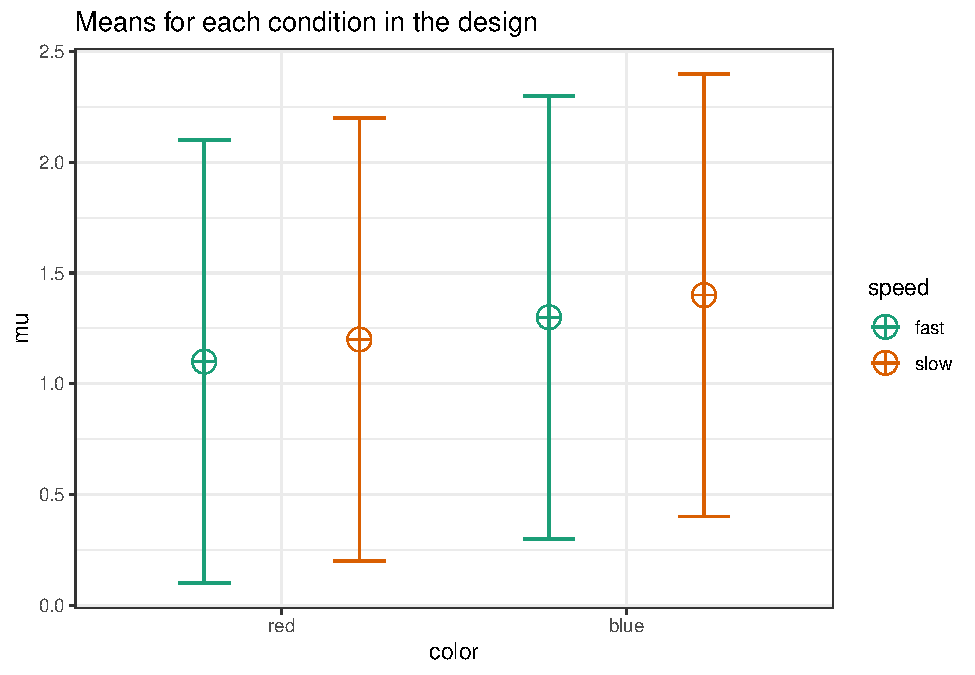
\includegraphics{SuperpowerValidation_files/figure-latex/unnamed-chunk-3-1.pdf}

\begin{Shaded}
\begin{Highlighting}[]
\NormalTok{alpha_level <-}\StringTok{ }\FloatTok{0.05}
\CommentTok{# You should think carefully about how to justify your alpha level.}
\CommentTok{# We will give some examples later, but for now, use 0.05.}
\KeywordTok{ANOVA_power}\NormalTok{(design_result, }\DataTypeTok{alpha_level =}\NormalTok{ alpha_level, }\DataTypeTok{nsims =}\NormalTok{ nsims)}
\end{Highlighting}
\end{Shaded}

\begin{verbatim}
## Power and Effect sizes for ANOVA tests
##                 power effect_size
## anova_condition    69     0.03316
## 
## Power and Effect sizes for contrasts
##                                   power effect_size
## p_condition_control_condition_pet    69       0.341
\end{verbatim}

The result shows that we have exactly the same power for the ANOVA, as we have for the \emph{t}-test. This is because when there are only two groups, these tests are mathematically identical. In a study with 100 participants, we would have quite low power (around 67.7\%). An ANOVA with 2 groups is identical to a \emph{t}-test. For our example, Cohen's d (the standardized mean difference) is 2.2/6.4, or d = 0.34375 for the difference between the control condition and pets, which we can use to easily compute the expected power for these simple comparisons using the pwr package.

\begin{Shaded}
\begin{Highlighting}[]
\KeywordTok{pwr.t.test}\NormalTok{(}\DataTypeTok{d =} \FloatTok{2.2}\OperatorTok{/}\FloatTok{6.4}\NormalTok{,}
           \DataTypeTok{n =} \DecValTok{100}\NormalTok{,}
           \DataTypeTok{sig.level =} \FloatTok{0.05}\NormalTok{,}
           \DataTypeTok{type=}\StringTok{"two.sample"}\NormalTok{,}
           \DataTypeTok{alternative=}\StringTok{"two.sided"}\NormalTok{)}\OperatorTok{$}\NormalTok{power}
\end{Highlighting}
\end{Shaded}

\begin{verbatim}
## [1] 0.6768572
\end{verbatim}

We can also directly compute Cohen's f from Cohen's d for two groups, as Cohen (1988) describes, because f = 1/2d. So f = 0.5*0.34375 = 0.171875. And indeed, power analysis using the pwr package yields the same result using the pwr.anova.test as the power.t.test.

\begin{Shaded}
\begin{Highlighting}[]
\NormalTok{K <-}\StringTok{ }\DecValTok{2}
\NormalTok{n <-}\StringTok{ }\DecValTok{100}
\NormalTok{f <-}\StringTok{ }\FloatTok{0.171875}
\KeywordTok{pwr.anova.test}\NormalTok{(}\DataTypeTok{n =}\NormalTok{ n,}
               \DataTypeTok{k =}\NormalTok{ K,}
               \DataTypeTok{f =}\NormalTok{ f,}
               \DataTypeTok{sig.level =}\NormalTok{ alpha_level)}\OperatorTok{$}\NormalTok{power}
\end{Highlighting}
\end{Shaded}

\begin{verbatim}
## [1] 0.6768572
\end{verbatim}

This analysis tells us that running the study with 100 participants in each condition is too likely to \emph{not} yield a significant test result, even if our expected pattern of differences is true. This is not optimal.

Let's mathematically explore which pattern of means we would need to expect to habe 90\% power for the ANOVA with 50 participants in each group. We can use the pwr package in R to compute a sensitivity analysis that tells us the effect size, in Cohen's f, that we are able to detect with 3 groups and 50 partiicpants in each group, in order to achive 90\% power with an alpha level of 5\%.

\begin{Shaded}
\begin{Highlighting}[]
\NormalTok{K <-}\StringTok{ }\DecValTok{2}
\NormalTok{n <-}\StringTok{ }\DecValTok{100}
\NormalTok{sd <-}\StringTok{ }\FloatTok{6.4}
\NormalTok{r <-}\StringTok{ }\DecValTok{0}
\CommentTok{#Calculate f when running simulation}
\NormalTok{f <-}\StringTok{ }\KeywordTok{pwr.anova.test}\NormalTok{(}\DataTypeTok{n =}\NormalTok{ n,}
                    \DataTypeTok{k =}\NormalTok{ K,}
                    \DataTypeTok{power =} \FloatTok{0.9}\NormalTok{,}
                    \DataTypeTok{sig.level =}\NormalTok{ alpha_level)}\OperatorTok{$}\NormalTok{f}
\NormalTok{f}
\end{Highlighting}
\end{Shaded}

\begin{verbatim}
## [1] 0.2303587
\end{verbatim}

This sensitivity analysis shows we have 90\% power in our planned design to detect effects of Cohen's f of 0.2303587. Benchmarks by Cohen (1988) for small, medium, and large Cohen's f values are 0.1, 0.25, and 0.4, which correspond to eta-squared values of small (.0099), medium (.0588), and large (.1379), in line with d = .2, .5, or .8. So, at least based on these benchmarks, we have 90\% power to detect effects that are slightly below a medium effect benchmark.

\begin{Shaded}
\begin{Highlighting}[]
\NormalTok{f2 <-}\StringTok{ }\NormalTok{f}\OperatorTok{^}\DecValTok{2}
\NormalTok{ES <-}\StringTok{ }\NormalTok{f2}\OperatorTok{/}\NormalTok{(f2}\OperatorTok{+}\DecValTok{1}\NormalTok{)}
\NormalTok{ES}
\end{Highlighting}
\end{Shaded}

\begin{verbatim}
## [1] 0.0503911
\end{verbatim}

Expressed in eta-squared, we can detect values of eta-squared = 0.05 or larger.

\begin{Shaded}
\begin{Highlighting}[]
\NormalTok{mu <-}\StringTok{ }\KeywordTok{mu_from_ES}\NormalTok{(}\DataTypeTok{K =}\NormalTok{ K, }\DataTypeTok{ES =}\NormalTok{ ES)}
\NormalTok{mu <-}\StringTok{ }\NormalTok{mu }\OperatorTok{*}\StringTok{ }\NormalTok{sd}
\NormalTok{mu}
\end{Highlighting}
\end{Shaded}

\begin{verbatim}
## [1] -1.474295  1.474295
\end{verbatim}

We can compute a pattern of means, given a standard deviation of 6.4, that would give us an effect size of f = 0.23, or eta-squared of 0.05. We should be able to accomplish this is the means are -1.474295 and 1.474295. We can use these values to confirm the ANOVA has 90\% power.

\begin{Shaded}
\begin{Highlighting}[]
\NormalTok{design_result <-}\StringTok{ }\KeywordTok{ANOVA_design}\NormalTok{(}\DataTypeTok{design =}\NormalTok{ string,}
                   \DataTypeTok{n =}\NormalTok{ n, }
                   \DataTypeTok{mu =}\NormalTok{ mu, }
                   \DataTypeTok{sd =}\NormalTok{ sd, }
                   \DataTypeTok{labelnames =}\NormalTok{ labelnames)}
\end{Highlighting}
\end{Shaded}

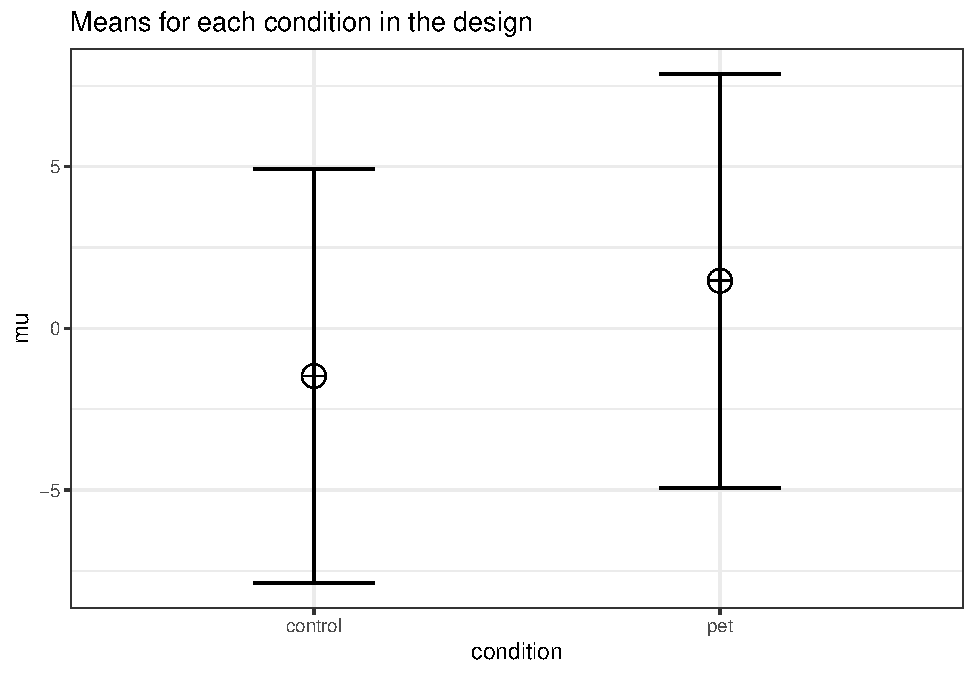
\includegraphics{SuperpowerValidation_files/figure-latex/unnamed-chunk-9-1.pdf}

\begin{Shaded}
\begin{Highlighting}[]
\KeywordTok{ANOVA_power}\NormalTok{(design_result, }\DataTypeTok{alpha_level =}\NormalTok{ alpha_level, }\DataTypeTok{nsims =}\NormalTok{ nsims)}
\end{Highlighting}
\end{Shaded}

\begin{verbatim}
## Power and Effect sizes for ANOVA tests
##                 power effect_size
## anova_condition    88     0.04836
## 
## Power and Effect sizes for contrasts
##                                   power effect_size
## p_condition_control_condition_pet    88      0.4328
\end{verbatim}

The simulation confirms that for the \emph{F}-test for the ANOVA we have 90\% power. This is also what g*power tells us what would happen based on a post-hoc power analysis with an f of 0.2303587, 2 groups, 200 participants in total (100 in each between subject condition), and an alpha of 5\%.

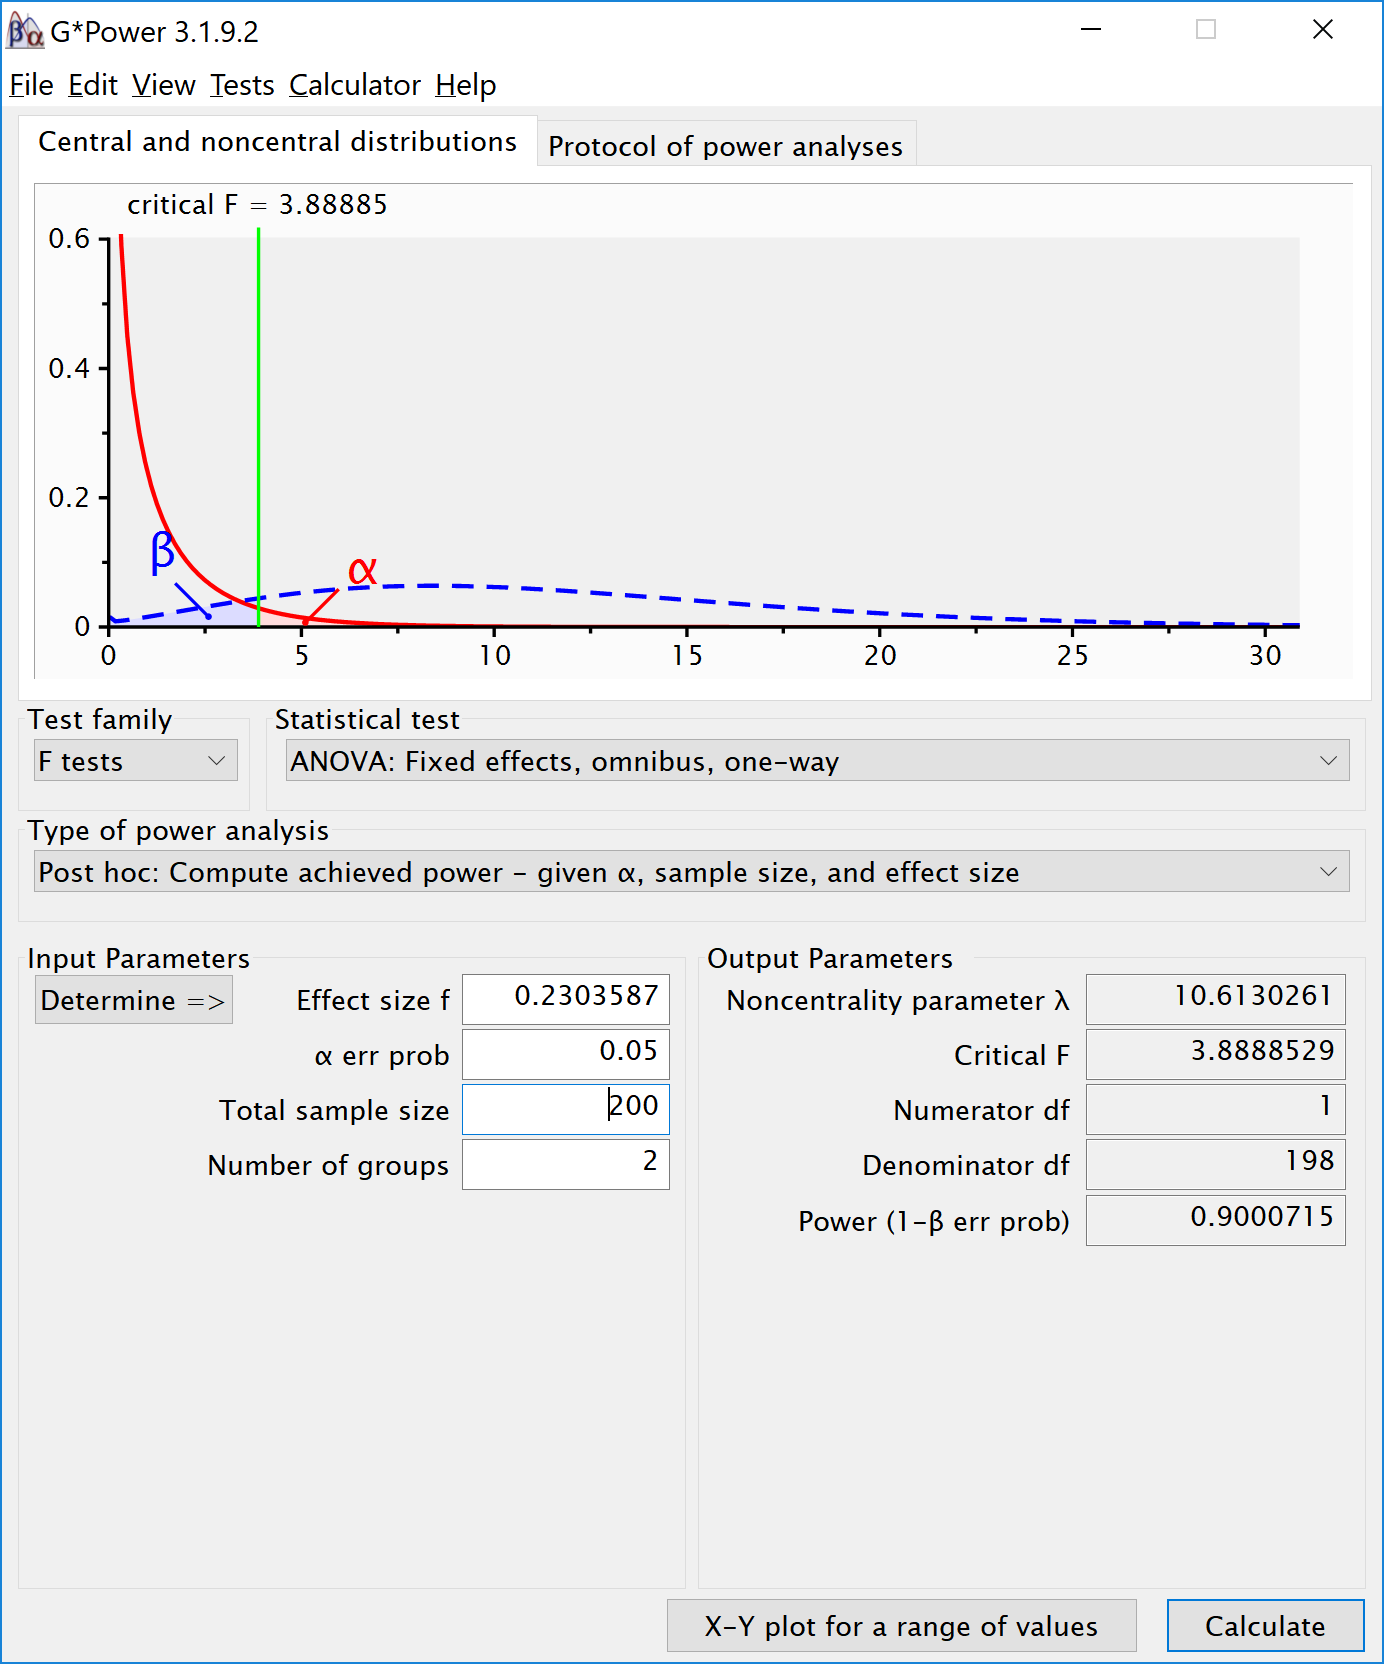
\includegraphics{screenshots/gpower_8.png}
If we return to our expected means, how many participants do we need for sufficient power? Given the expected difference and standard deviation, d = 0.34375, and f = 0.171875. We can perform an a-priori power analysis for this simple case, which tells us we need 179 participants in each group (we can't split people in parts, and thus always round a power analysis upward), or 358 in total.

\begin{Shaded}
\begin{Highlighting}[]
\NormalTok{K <-}\StringTok{ }\DecValTok{2}
\NormalTok{power <-}\StringTok{ }\FloatTok{0.9}
\NormalTok{f <-}\StringTok{ }\FloatTok{0.171875}
\KeywordTok{pwr.anova.test}\NormalTok{(}\DataTypeTok{power =}\NormalTok{ power,}
               \DataTypeTok{k =}\NormalTok{ K,}
               \DataTypeTok{f =}\NormalTok{ f,}
               \DataTypeTok{sig.level =}\NormalTok{ alpha_level)}
\end{Highlighting}
\end{Shaded}

\begin{verbatim}
## 
##      Balanced one-way analysis of variance power calculation 
## 
##               k = 2
##               n = 178.8104
##               f = 0.171875
##       sig.level = 0.05
##           power = 0.9
## 
## NOTE: n is number in each group
\end{verbatim}

If we re-run the simulation with this sample size, we indeed have 90\% power.

\begin{Shaded}
\begin{Highlighting}[]
\NormalTok{string <-}\StringTok{ "2b"}
\NormalTok{n <-}\StringTok{ }\DecValTok{179}
\NormalTok{mu <-}\StringTok{ }\KeywordTok{c}\NormalTok{(}\DecValTok{24}\NormalTok{, }\FloatTok{26.2}\NormalTok{)}
\CommentTok{# Enter means in the order that matches the labels below.}
\CommentTok{# In this case, control, pet. }
\NormalTok{sd <-}\StringTok{ }\FloatTok{6.4}
\NormalTok{labelnames <-}\StringTok{ }\KeywordTok{c}\NormalTok{(}\StringTok{"condition"}\NormalTok{, }\StringTok{"control"}\NormalTok{, }\StringTok{"pet"}\NormalTok{) }\CommentTok{#}
\CommentTok{# the label names should be in the order of the means specified above.}
\NormalTok{design_result <-}\StringTok{ }\KeywordTok{ANOVA_design}\NormalTok{(}\DataTypeTok{design =}\NormalTok{ string,}
                   \DataTypeTok{n =}\NormalTok{ n, }
                   \DataTypeTok{mu =}\NormalTok{ mu, }
                   \DataTypeTok{sd =}\NormalTok{ sd, }
                   \DataTypeTok{labelnames =}\NormalTok{ labelnames)}
\end{Highlighting}
\end{Shaded}

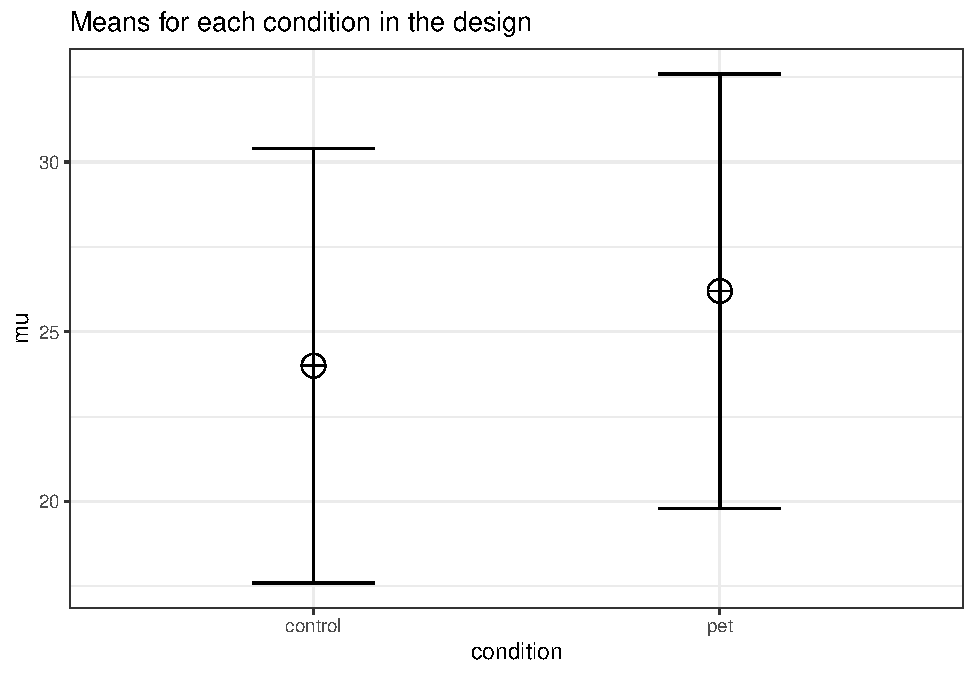
\includegraphics{SuperpowerValidation_files/figure-latex/unnamed-chunk-11-1.pdf}

\begin{Shaded}
\begin{Highlighting}[]
\NormalTok{alpha_level <-}\StringTok{ }\FloatTok{0.05}
\NormalTok{power_result <-}\StringTok{ }\KeywordTok{ANOVA_power}\NormalTok{(design_result, }\DataTypeTok{alpha_level =}\NormalTok{ alpha_level, }\DataTypeTok{nsims =}\NormalTok{ nsims)}
\end{Highlighting}
\end{Shaded}

\begin{verbatim}
## Power and Effect sizes for ANOVA tests
##                 power effect_size
## anova_condition    88     0.03289
## 
## Power and Effect sizes for contrasts
##                                   power effect_size
## p_condition_control_condition_pet    88      0.3533
\end{verbatim}

We stored the result from the power analysis in an object. This allows us to request plots (which are not printed automatically) showing the \emph{p}-value distribution. If we request power\_result\$plot1 we get the p-value distribution for the ANOVA:

\begin{Shaded}
\begin{Highlighting}[]
\NormalTok{power_result}\OperatorTok{$}\NormalTok{plot1}
\end{Highlighting}
\end{Shaded}

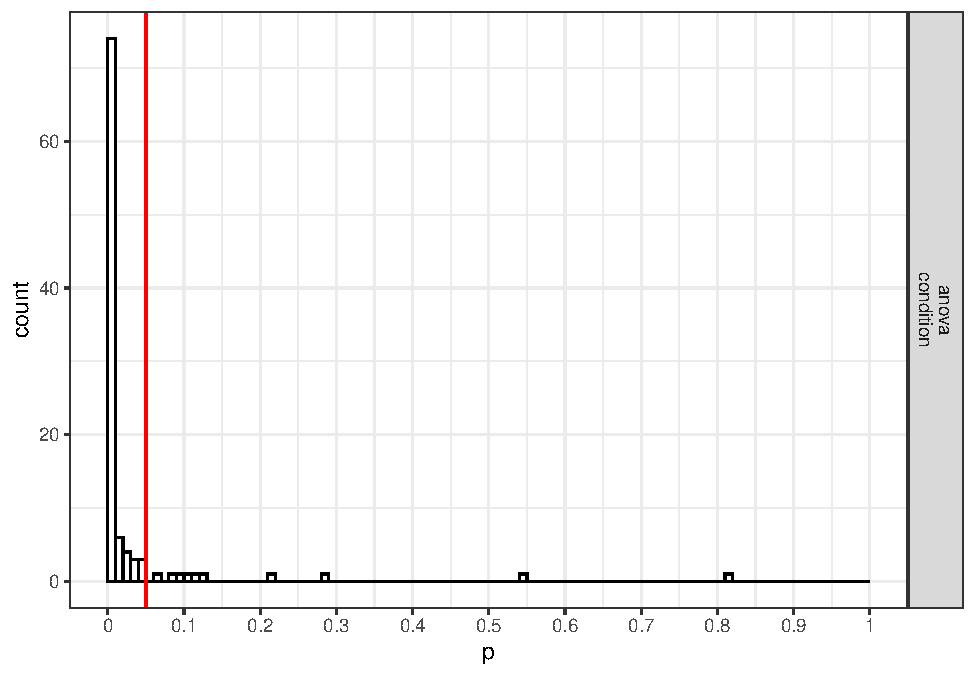
\includegraphics{SuperpowerValidation_files/figure-latex/unnamed-chunk-12-1.pdf}
If we request power\_result\$plot2 we get the p-value distribution for the paired comparisons (in this case only one):

\begin{Shaded}
\begin{Highlighting}[]
\NormalTok{power_result}\OperatorTok{$}\NormalTok{plot2}
\end{Highlighting}
\end{Shaded}

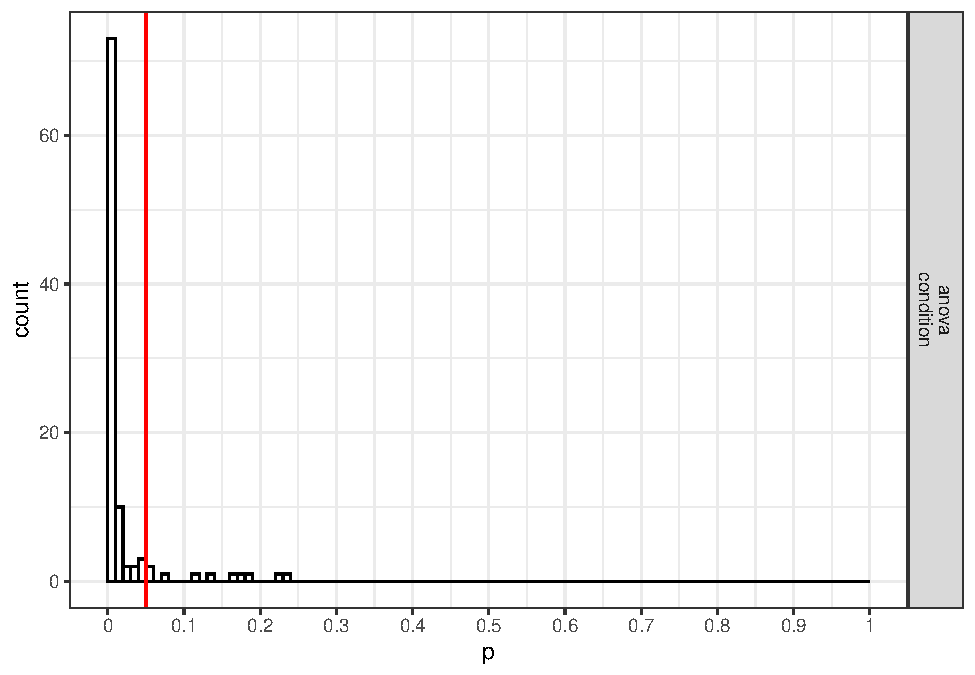
\includegraphics{SuperpowerValidation_files/figure-latex/unnamed-chunk-13-1.pdf}

\hypertarget{one-way-anova-part-2}{%
\chapter{One-way ANOVA Part 2}\label{one-way-anova-part-2}}

\hypertarget{validation-of-power-in-one-way-anova-with-brysbaert-example}{%
\section{Validation of Power in One-Way ANOVA with Brysbaert example}\label{validation-of-power-in-one-way-anova-with-brysbaert-example}}

\hypertarget{three-conditions}{%
\subsection{Three conditions}\label{three-conditions}}

Imagine we aim to design a study to test the hypothesis that giving people a pet to take care of will increase their life satisfaction. We have a control condition, a `cat' pet condition, and a `dog' pet condition. We can simulate a One-Way ANOVA with a specified alpha, sample size, and effect size, on see the statistical power we would have for the ANOVA and the follow-up comparisons. We expect all pets to increase life-satisfaction compared to the control condition. Obviously, we also expect the people who are in the `dog' pet condition to have even greater life-satisfaction than people in the `cat' pet condition. Based on work by Pavot and Diener (1993) we believe that we can expect responses on the life-satifaction scale to have a mean of approximately 24 in our population, with a standard deviation of 6.4. We expect having a pet increases life satisfaction with approximately 2.2 scale points for participants who get a cat, and 2.6 scale points for participants who get a dog. We initially consider collecting data from 150 participants in total, with 50 participants in each condition. But before we proceed with the data collection, we examine the statistical power our design would have to detect the differences we predict.

\begin{Shaded}
\begin{Highlighting}[]
\NormalTok{string <-}\StringTok{ "3b"}
\NormalTok{n <-}\StringTok{ }\DecValTok{50}
\CommentTok{# We are thinking of running 50 peope in each condition}
\NormalTok{mu <-}\StringTok{ }\KeywordTok{c}\NormalTok{(}\DecValTok{24}\NormalTok{, }\FloatTok{26.2}\NormalTok{, }\FloatTok{26.6}\NormalTok{)}
\CommentTok{# Enter means in the order that matches the labels below.}
\CommentTok{# In this case, control, cat, dog. }
\NormalTok{sd <-}\StringTok{ }\FloatTok{6.4}
\NormalTok{labelnames <-}\StringTok{ }\KeywordTok{c}\NormalTok{(}\StringTok{"condition"}\NormalTok{, }\StringTok{"control"}\NormalTok{, }\StringTok{"cat"}\NormalTok{, }\StringTok{"dog"}\NormalTok{) }\CommentTok{#}
\CommentTok{# the label names should be in the order of the means specified above.}
\NormalTok{design_result <-}\StringTok{ }\KeywordTok{ANOVA_design}\NormalTok{(}\DataTypeTok{design =}\NormalTok{ string,}
                   \DataTypeTok{n =}\NormalTok{ n, }
                   \DataTypeTok{mu =}\NormalTok{ mu, }
                   \DataTypeTok{sd =}\NormalTok{ sd, }
                   \DataTypeTok{labelnames =}\NormalTok{ labelnames)}
\end{Highlighting}
\end{Shaded}

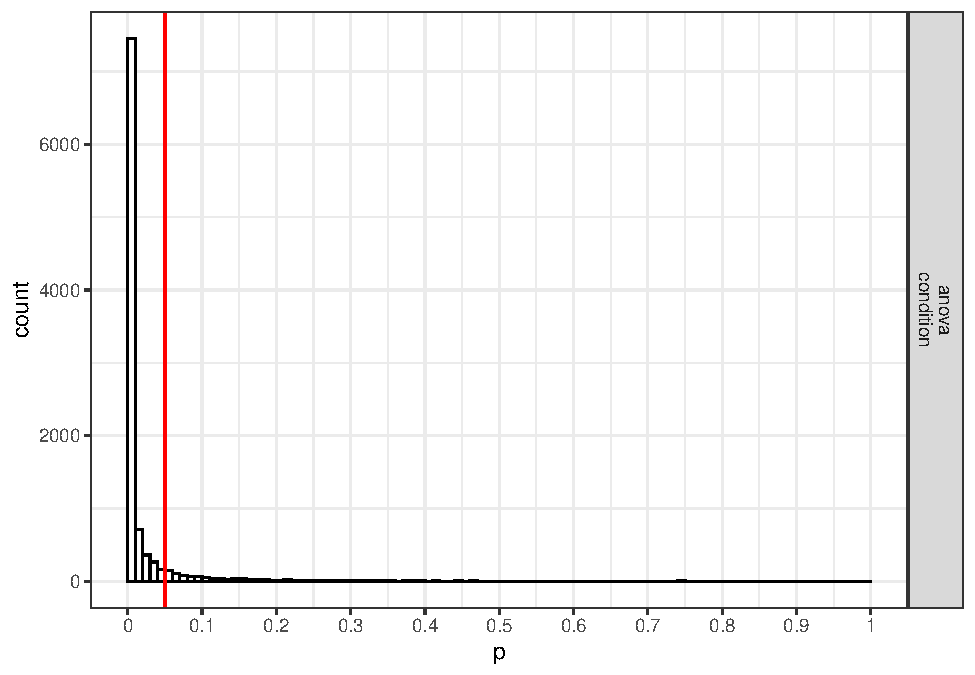
\includegraphics{SuperpowerValidation_files/figure-latex/unnamed-chunk-15-1.pdf}

\begin{Shaded}
\begin{Highlighting}[]
\NormalTok{alpha_level <-}\StringTok{ }\FloatTok{0.05}
\CommentTok{# You should think carefully about how to justify your alpha level.}
\CommentTok{# We will give some examples later, but for now, use 0.05.}
\KeywordTok{ANOVA_power}\NormalTok{(design_result, }\DataTypeTok{alpha_level =}\NormalTok{ alpha_level, }\DataTypeTok{nsims =}\NormalTok{ nsims)}
\end{Highlighting}
\end{Shaded}

\begin{verbatim}
## Power and Effect sizes for ANOVA tests
##                 power effect_size
## anova_condition    46     0.04169
## 
## Power and Effect sizes for contrasts
##                                   power effect_size
## p_condition_control_condition_cat    41     0.33459
## p_condition_control_condition_dog    46     0.37274
## p_condition_cat_condition_dog         7     0.03855
\end{verbatim}

\begin{Shaded}
\begin{Highlighting}[]
\CommentTok{#should yield}
\CommentTok{#0.3983064}
\CommentTok{#0.5205162}
\CommentTok{#0.06104044}
\end{Highlighting}
\end{Shaded}

The result shows that you would have quite low power with 50 participants, both for the overall ANOVA (just around 50\% power), as for the follow up comparisons (approximately 40\% power for the control vs cat condition, around 50\% for the control vs dogs condition, and a really low power (around 6\%, just above the Type 1 error rate of 5\%) for the expected difference between cats and dogs.

\hypertarget{power-for-simple-effects}{%
\section{Power for simple effects}\label{power-for-simple-effects}}

We are typically not just interested in the ANOVA, but also in follow up comparisons. In this case, we would perform a \emph{t}-test comparing the control condition against the cat and dog condition, and we would compare the cat and dog conditions against each other, in independent \emph{t}-tests.

For our example, Cohen's d (the standardized mean difference) is 2.2/6.4, or d = 0.34375 for the difference between the control condition and cats, 2.6/6.4 of d = 0.40625 for the difference between the control condition and dogs, and 0.4/6.4 or d = 0.0625 for the difference between cats and dogs as pets.

We can easily compute the expected power for these simple comparisons using the pwr package.

\begin{Shaded}
\begin{Highlighting}[]
\KeywordTok{pwr.t.test}\NormalTok{(}\DataTypeTok{d =} \FloatTok{2.2}\OperatorTok{/}\FloatTok{6.4}\NormalTok{,}
           \DataTypeTok{n =} \DecValTok{50}\NormalTok{,}
           \DataTypeTok{sig.level =} \FloatTok{0.05}\NormalTok{,}
           \DataTypeTok{type=}\StringTok{"two.sample"}\NormalTok{,}
           \DataTypeTok{alternative=}\StringTok{"two.sided"}\NormalTok{)}\OperatorTok{$}\NormalTok{power}
\end{Highlighting}
\end{Shaded}

\begin{verbatim}
## [1] 0.3983064
\end{verbatim}

\begin{Shaded}
\begin{Highlighting}[]
\KeywordTok{pwr.t.test}\NormalTok{(}\DataTypeTok{d =} \FloatTok{2.6}\OperatorTok{/}\FloatTok{6.4}\NormalTok{,}
           \DataTypeTok{n =} \DecValTok{50}\NormalTok{,}
           \DataTypeTok{sig.level =} \FloatTok{0.05}\NormalTok{,}
           \DataTypeTok{type=}\StringTok{"two.sample"}\NormalTok{,}
           \DataTypeTok{alternative=}\StringTok{"two.sided"}\NormalTok{)}\OperatorTok{$}\NormalTok{power}
\end{Highlighting}
\end{Shaded}

\begin{verbatim}
## [1] 0.5205162
\end{verbatim}

\begin{Shaded}
\begin{Highlighting}[]
\KeywordTok{pwr.t.test}\NormalTok{(}\DataTypeTok{d =} \FloatTok{0.4}\OperatorTok{/}\FloatTok{6.4}\NormalTok{,}
           \DataTypeTok{n =} \DecValTok{50}\NormalTok{,}
           \DataTypeTok{sig.level =} \FloatTok{0.05}\NormalTok{,}
           \DataTypeTok{type=}\StringTok{"two.sample"}\NormalTok{,}
           \DataTypeTok{alternative=}\StringTok{"two.sided"}\NormalTok{)}\OperatorTok{$}\NormalTok{power}
\end{Highlighting}
\end{Shaded}

\begin{verbatim}
## [1] 0.06104044
\end{verbatim}

This analysis tells us that running the study with 50 participants in each condition is more likely to \emph{not} yield a significant test result, even if our expected pattern of differences is true, than that we will observe a \emph{p}-value smaller than our alpha level. This is not optimal.

Let's mathematically explore which pattern of means we would need to expect to habe 90\% power for the ANOVA with 50 participants in each group. We can use the pwr package in R to compute a sensitivity analysis that tells us the effect size, in Cohen's f, that we are able to detect with 3 groups and 50 partiicpants in each group, in order to achive 90\% power with an alpha level of 5\%.

\begin{Shaded}
\begin{Highlighting}[]
\NormalTok{K <-}\StringTok{ }\DecValTok{3}
\NormalTok{n <-}\StringTok{ }\DecValTok{50}
\NormalTok{sd <-}\StringTok{ }\FloatTok{6.4}
\NormalTok{r <-}\StringTok{ }\DecValTok{0}
\CommentTok{#Calculate f when running simulation}
\NormalTok{f <-}\StringTok{ }\KeywordTok{pwr.anova.test}\NormalTok{(}\DataTypeTok{n =}\NormalTok{ n,}
                    \DataTypeTok{k =}\NormalTok{ K,}
                    \DataTypeTok{power =} \FloatTok{0.9}\NormalTok{,}
                    \DataTypeTok{sig.level =}\NormalTok{ alpha_level)}\OperatorTok{$}\NormalTok{f}
\NormalTok{f}
\end{Highlighting}
\end{Shaded}

\begin{verbatim}
## [1] 0.2934417
\end{verbatim}

This sensitivity analysis shows we have 90\% power in our planned design to detect effects of Cohen's f of 0.2934417. Benchmarks by Cohen (1988) for small, medium, and large Cohen's f values are 0.1, 0.25, and 0.4, which correspond to eta-squared values of small (.0099), medium (.0588), and large (.1379), in line with d = .2, .5, or .8. So, at least based on these benchmarks, we have 90\% power to detect effects that are somewhat sizeable.

\begin{Shaded}
\begin{Highlighting}[]
\NormalTok{f2 <-}\StringTok{ }\NormalTok{f}\OperatorTok{^}\DecValTok{2}
\NormalTok{ES <-}\StringTok{ }\NormalTok{f2}\OperatorTok{/}\NormalTok{(f2}\OperatorTok{+}\DecValTok{1}\NormalTok{)}
\NormalTok{ES}
\end{Highlighting}
\end{Shaded}

\begin{verbatim}
## [1] 0.07928127
\end{verbatim}

Expressed in eta-squared, we can detect values of eta-squared = 0.0793 or larger.

\begin{Shaded}
\begin{Highlighting}[]
\NormalTok{mu <-}\StringTok{ }\KeywordTok{mu_from_ES}\NormalTok{(}\DataTypeTok{K =}\NormalTok{ K, }\DataTypeTok{ES =}\NormalTok{ ES)}
\NormalTok{mu <-}\StringTok{ }\NormalTok{mu }\OperatorTok{*}\StringTok{ }\NormalTok{sd}
\NormalTok{mu}
\end{Highlighting}
\end{Shaded}

\begin{verbatim}
## [1] -2.300104  0.000000  2.300104
\end{verbatim}

We can compute a pattern of means, given a standard deviation of 6.4, that would give us an effect size of f = 0.2934, or eta-squared of 0.0793. We should be able to accomplish this is the means are -2.300104, 0.000000, and 2.300104. We can use these values to confirm the ANOVA has 90\% power.

\begin{Shaded}
\begin{Highlighting}[]
\NormalTok{design_result <-}\StringTok{ }\KeywordTok{ANOVA_design}\NormalTok{(}\DataTypeTok{design =}\NormalTok{ string,}
                   \DataTypeTok{n =}\NormalTok{ n, }
                   \DataTypeTok{mu =}\NormalTok{ mu, }
                   \DataTypeTok{sd =}\NormalTok{ sd, }
                   \DataTypeTok{labelnames =}\NormalTok{ labelnames)}
\end{Highlighting}
\end{Shaded}

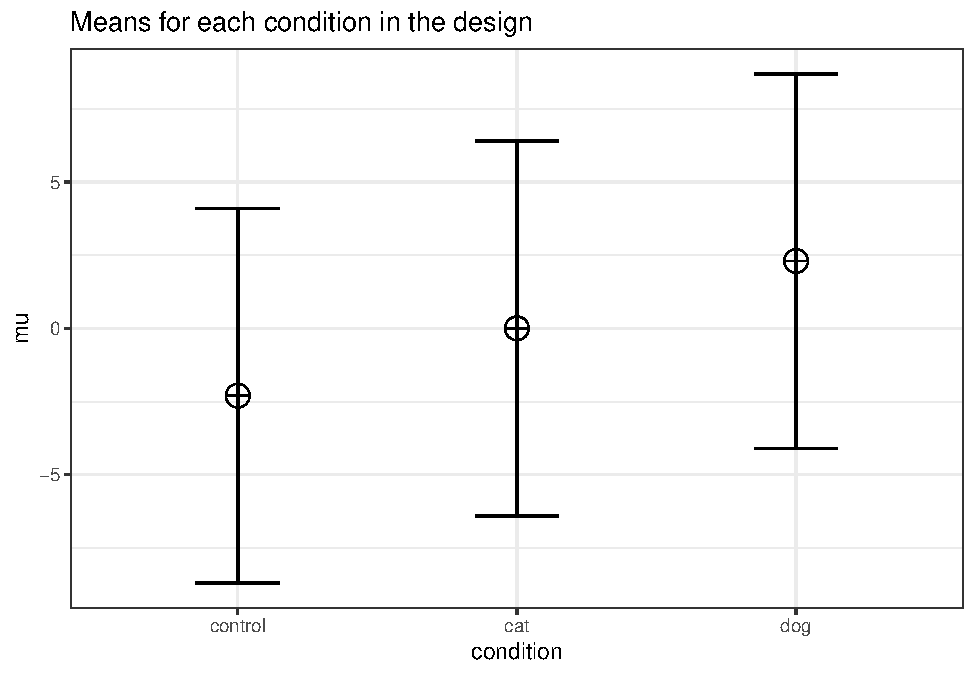
\includegraphics{SuperpowerValidation_files/figure-latex/unnamed-chunk-20-1.pdf}

\begin{Shaded}
\begin{Highlighting}[]
\KeywordTok{ANOVA_power}\NormalTok{(design_result, }\DataTypeTok{alpha_level =}\NormalTok{ alpha_level, }\DataTypeTok{nsims =}\NormalTok{ nsims)}
\end{Highlighting}
\end{Shaded}

\begin{verbatim}
## Power and Effect sizes for ANOVA tests
##                 power effect_size
## anova_condition    88     0.08837
## 
## Power and Effect sizes for contrasts
##                                   power effect_size
## p_condition_control_condition_cat    48      0.3741
## p_condition_control_condition_dog    91      0.7049
## p_condition_cat_condition_dog        39      0.3247
\end{verbatim}

The simulation confirms that for the \emph{F}-test for the ANOVA we have 90\% power. This is also what g*power tells us what would happen based on a post-hoc power analysis with an f of 0.2934417, 3 groups, 150 participants in total (50 in each between subject condition), and an alpha of 5\%.

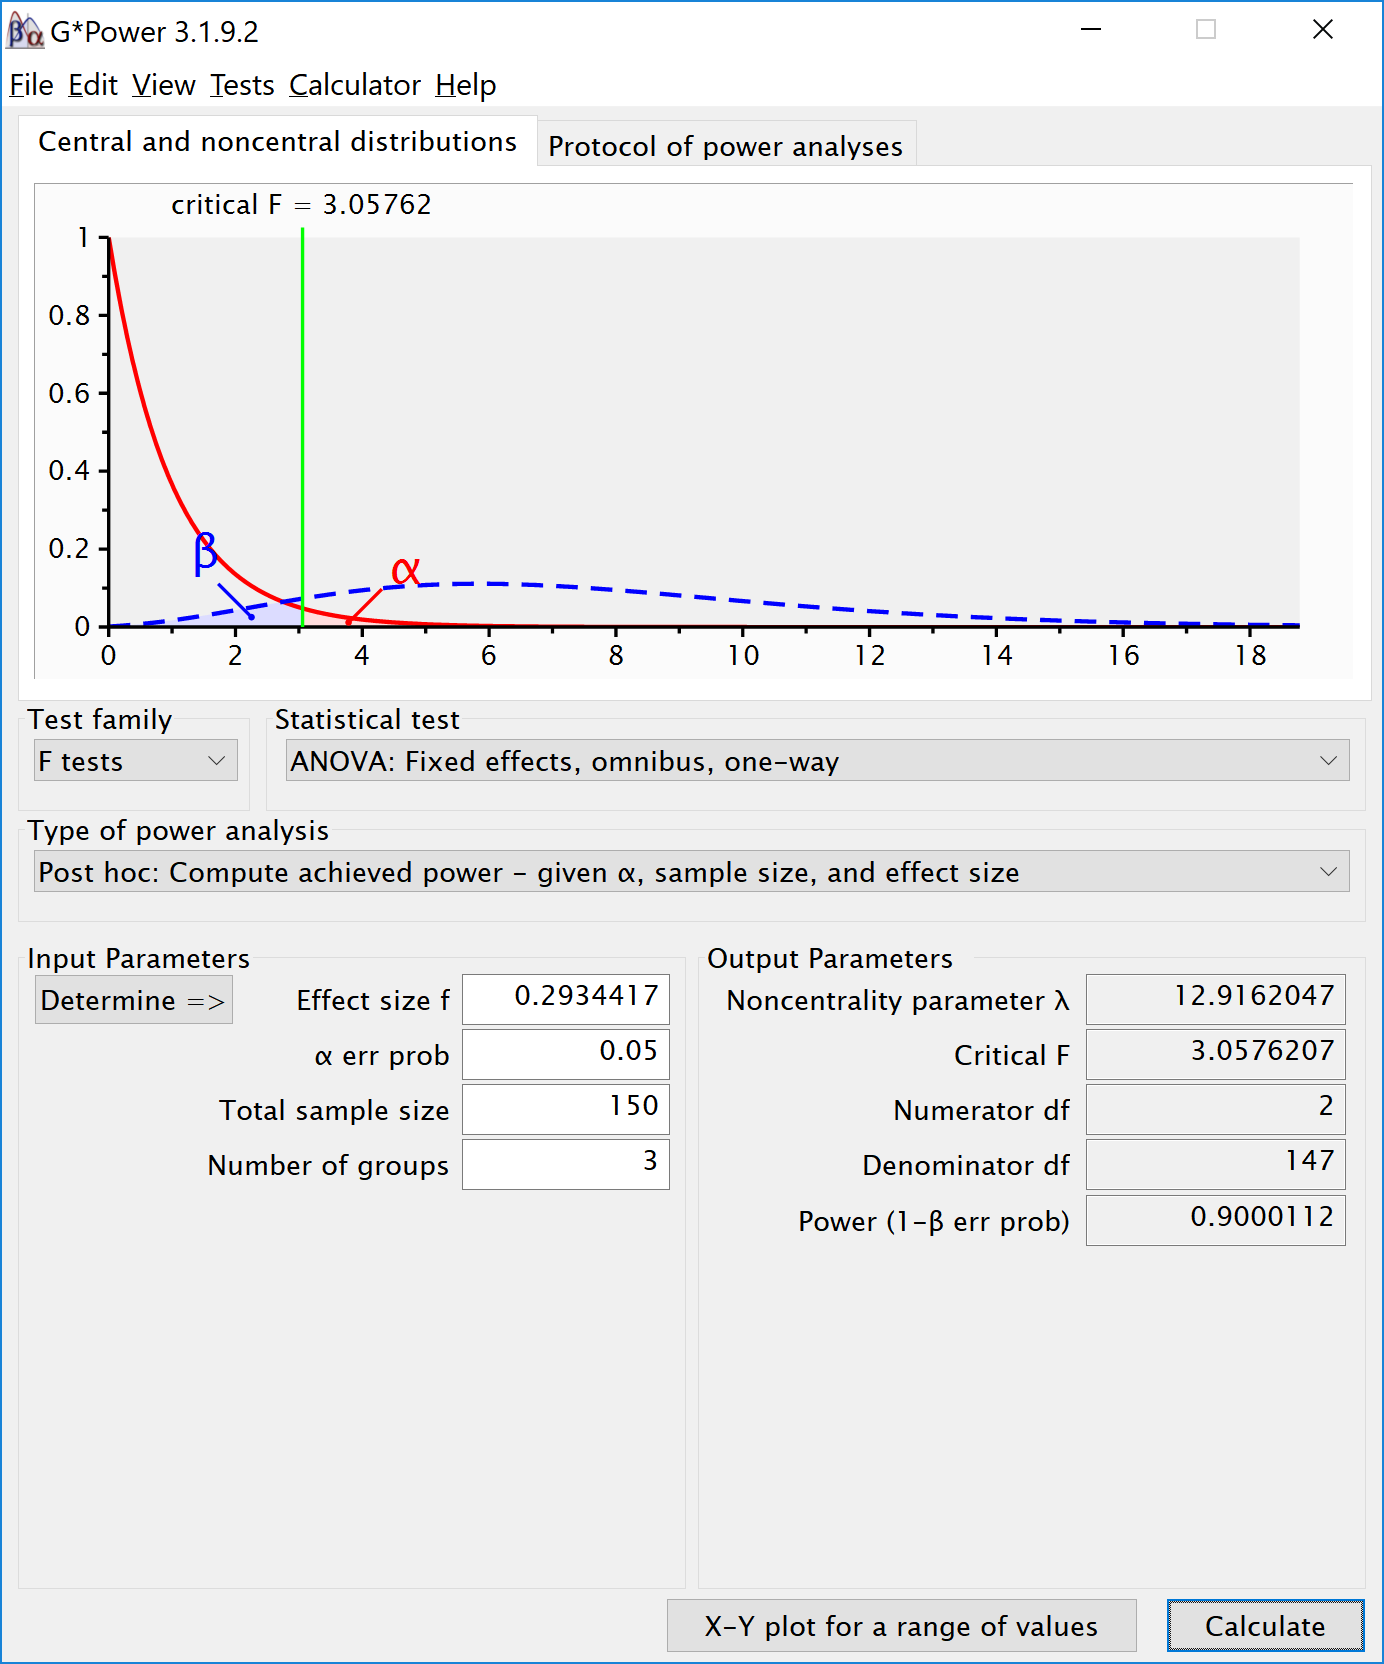
\includegraphics{screenshots/gpower_7.png}

We can also compute the power for the ANOVA and simple effects in R with the pwr package. The calculated effect sizes and power match those from the simulation.

\begin{Shaded}
\begin{Highlighting}[]
\NormalTok{K <-}\StringTok{ }\DecValTok{3}
\NormalTok{n <-}\StringTok{ }\DecValTok{50}
\NormalTok{sd <-}\StringTok{ }\FloatTok{6.4}
\NormalTok{f <-}\StringTok{ }\FloatTok{0.2934417}
\KeywordTok{pwr.anova.test}\NormalTok{(}\DataTypeTok{n =}\NormalTok{ n,}
               \DataTypeTok{k =}\NormalTok{ K,}
               \DataTypeTok{f =}\NormalTok{ f,}
               \DataTypeTok{sig.level =}\NormalTok{ alpha_level)}\OperatorTok{$}\NormalTok{power}
\end{Highlighting}
\end{Shaded}

\begin{verbatim}
## [1] 0.9000112
\end{verbatim}

\begin{Shaded}
\begin{Highlighting}[]
\NormalTok{d <-}\StringTok{ }\FloatTok{2.300104}\OperatorTok{/}\FloatTok{6.4}
\NormalTok{d}
\end{Highlighting}
\end{Shaded}

\begin{verbatim}
## [1] 0.3593912
\end{verbatim}

\begin{Shaded}
\begin{Highlighting}[]
\KeywordTok{pwr.t.test}\NormalTok{(}\DataTypeTok{d =} \FloatTok{2.300104}\OperatorTok{/}\FloatTok{6.4}\NormalTok{,}
           \DataTypeTok{n =} \DecValTok{50}\NormalTok{,}
           \DataTypeTok{sig.level =} \FloatTok{0.05}\NormalTok{,}
           \DataTypeTok{type=}\StringTok{"two.sample"}\NormalTok{,}
           \DataTypeTok{alternative=}\StringTok{"two.sided"}\NormalTok{)}\OperatorTok{$}\NormalTok{power}
\end{Highlighting}
\end{Shaded}

\begin{verbatim}
## [1] 0.4284243
\end{verbatim}

\begin{Shaded}
\begin{Highlighting}[]
\NormalTok{d <-}\StringTok{ }\DecValTok{2}\OperatorTok{*}\FloatTok{2.300104}\OperatorTok{/}\FloatTok{6.4}
\NormalTok{d}
\end{Highlighting}
\end{Shaded}

\begin{verbatim}
## [1] 0.7187825
\end{verbatim}

\begin{Shaded}
\begin{Highlighting}[]
\KeywordTok{pwr.t.test}\NormalTok{(}\DataTypeTok{d =}\NormalTok{ d,}
           \DataTypeTok{n =} \DecValTok{50}\NormalTok{,}
           \DataTypeTok{sig.level =} \FloatTok{0.05}\NormalTok{,}
           \DataTypeTok{type=}\StringTok{"two.sample"}\NormalTok{,}
           \DataTypeTok{alternative=}\StringTok{"two.sided"}\NormalTok{)}\OperatorTok{$}\NormalTok{power}
\end{Highlighting}
\end{Shaded}

\begin{verbatim}
## [1] 0.9450353
\end{verbatim}

We can also compare the results against the analytic solution by Aberson (2019).

First, load the function for a 3-way ANOVA.

\begin{Shaded}
\begin{Highlighting}[]
\NormalTok{anova1f_}\DecValTok{3}\NormalTok{<-}\ControlFlowTok{function}\NormalTok{(}\DataTypeTok{m1=}\OtherTok{NULL}\NormalTok{,}\DataTypeTok{m2=}\OtherTok{NULL}\NormalTok{,}\DataTypeTok{m3=}\OtherTok{NULL}\NormalTok{,}\DataTypeTok{s1=}\OtherTok{NULL}\NormalTok{,}\DataTypeTok{s2=}\OtherTok{NULL}\NormalTok{,}\DataTypeTok{s3=}\OtherTok{NULL}\NormalTok{,}\DataTypeTok{n1=}\OtherTok{NULL}\NormalTok{,}\DataTypeTok{n2=}\OtherTok{NULL}\NormalTok{,}\DataTypeTok{n3=}\OtherTok{NULL}\NormalTok{,}\DataTypeTok{alpha=}\NormalTok{.}\DecValTok{05}\NormalTok{)\{}
\NormalTok{x<-stats}\OperatorTok{::}\KeywordTok{rnorm}\NormalTok{(n1,m1,s1)}
\NormalTok{X<-x}
\NormalTok{MEAN<-m1}
\NormalTok{SD<-s1}
\NormalTok{Z <-}\StringTok{ }\NormalTok{(((X }\OperatorTok{-}\StringTok{ }\KeywordTok{mean}\NormalTok{(X, }\DataTypeTok{na.rm =} \OtherTok{TRUE}\NormalTok{))}\OperatorTok{/}\NormalTok{stats}\OperatorTok{::}\KeywordTok{sd}\NormalTok{(X, }\DataTypeTok{na.rm =} \OtherTok{TRUE}\NormalTok{))) }\OperatorTok{*}\StringTok{ }\NormalTok{SD}
\NormalTok{y<-MEAN }\OperatorTok{+}\StringTok{ }\NormalTok{Z}
\NormalTok{group<-}\KeywordTok{rep}\NormalTok{(}\StringTok{"A1"}\NormalTok{,n1)}
\NormalTok{l1<-}\KeywordTok{data.frame}\NormalTok{(y, group)}
\NormalTok{x<-stats}\OperatorTok{::}\KeywordTok{rnorm}\NormalTok{(n2,m2,s2)}
\NormalTok{X<-x}
\NormalTok{MEAN<-m2}
\NormalTok{SD<-s2}
\NormalTok{Z <-}\StringTok{ }\NormalTok{(((X }\OperatorTok{-}\StringTok{ }\KeywordTok{mean}\NormalTok{(X, }\DataTypeTok{na.rm =} \OtherTok{TRUE}\NormalTok{))}\OperatorTok{/}\NormalTok{stats}\OperatorTok{::}\KeywordTok{sd}\NormalTok{(X, }\DataTypeTok{na.rm =} \OtherTok{TRUE}\NormalTok{))) }\OperatorTok{*}\StringTok{ }\NormalTok{SD}
\NormalTok{y<-MEAN }\OperatorTok{+}\StringTok{ }\NormalTok{Z}
\NormalTok{group<-}\KeywordTok{rep}\NormalTok{(}\StringTok{"A2"}\NormalTok{,n2)}
\NormalTok{l2<-}\KeywordTok{data.frame}\NormalTok{(y, group)}
\NormalTok{x<-stats}\OperatorTok{::}\KeywordTok{rnorm}\NormalTok{(n3,m3,s3)}
\NormalTok{X<-x}
\NormalTok{MEAN<-m3}
\NormalTok{SD<-s3}
\NormalTok{Z <-}\StringTok{ }\NormalTok{(((X }\OperatorTok{-}\StringTok{ }\KeywordTok{mean}\NormalTok{(X, }\DataTypeTok{na.rm =} \OtherTok{TRUE}\NormalTok{))}\OperatorTok{/}\NormalTok{stats}\OperatorTok{::}\KeywordTok{sd}\NormalTok{(X, }\DataTypeTok{na.rm =} \OtherTok{TRUE}\NormalTok{))) }\OperatorTok{*}\StringTok{ }\NormalTok{SD}
\NormalTok{y<-MEAN }\OperatorTok{+}\StringTok{ }\NormalTok{Z}
\NormalTok{group<-}\KeywordTok{rep}\NormalTok{(}\StringTok{"A3"}\NormalTok{,n3)}
\NormalTok{l3<-}\KeywordTok{data.frame}\NormalTok{(y, group)}
\NormalTok{simdat<-}\KeywordTok{rbind}\NormalTok{(l1,l2,l3)}
\NormalTok{anova<-stats}\OperatorTok{::}\KeywordTok{aov}\NormalTok{(y}\OperatorTok{~}\NormalTok{group, }\DataTypeTok{data=}\NormalTok{simdat)}
\NormalTok{anova<-car}\OperatorTok{::}\KeywordTok{Anova}\NormalTok{(anova, }\DataTypeTok{type=}\StringTok{"III"}\NormalTok{)}
\NormalTok{SSA<-anova[}\DecValTok{2}\NormalTok{,}\DecValTok{1}\NormalTok{] }\CommentTok{#column, row}
\NormalTok{SSwin<-anova[}\DecValTok{3}\NormalTok{,}\DecValTok{1}\NormalTok{]}
\NormalTok{dfwin<-anova[}\DecValTok{3}\NormalTok{,}\DecValTok{2}\NormalTok{]}
\NormalTok{dfbg<-anova[}\DecValTok{2}\NormalTok{,}\DecValTok{2}\NormalTok{]}
\NormalTok{eta2<-SSA}\OperatorTok{/}\NormalTok{(SSA}\OperatorTok{+}\NormalTok{SSwin)}
\NormalTok{f2<-eta2}\OperatorTok{/}\NormalTok{(}\DecValTok{1}\OperatorTok{-}\NormalTok{eta2)}
\NormalTok{lambda<-f2}\OperatorTok{*}\NormalTok{dfwin}
\NormalTok{minusalpha<-}\DecValTok{1}\OperatorTok{-}\NormalTok{alpha}
\NormalTok{Ft<-stats}\OperatorTok{::}\KeywordTok{qf}\NormalTok{(minusalpha, dfbg, dfwin)}
\NormalTok{power<-}\DecValTok{1}\OperatorTok{-}\NormalTok{stats}\OperatorTok{::}\KeywordTok{pf}\NormalTok{(Ft, dfbg,dfwin,lambda)}
\KeywordTok{list}\NormalTok{(}\DataTypeTok{Power =}\NormalTok{ power)\}}
\end{Highlighting}
\end{Shaded}

Then we use the function to calculate power.

\begin{Shaded}
\begin{Highlighting}[]
\CommentTok{#Initial example, low power}
\KeywordTok{anova1f_3}\NormalTok{(}\DataTypeTok{m1=}\DecValTok{24}\NormalTok{, }\DataTypeTok{m2=}\FloatTok{26.2}\NormalTok{, }\DataTypeTok{m3=}\FloatTok{26.6}\NormalTok{, }\DataTypeTok{s1=}\FloatTok{6.4}\NormalTok{, }\DataTypeTok{s2=}\FloatTok{6.4}\NormalTok{, }\DataTypeTok{s3=}\FloatTok{6.4}\NormalTok{, }\DataTypeTok{n1=}\DecValTok{50}\NormalTok{, }\DataTypeTok{n2=}\DecValTok{50}\NormalTok{, }\DataTypeTok{n3=}\DecValTok{50}\NormalTok{, }\DataTypeTok{alpha=}\NormalTok{.}\DecValTok{05}\NormalTok{)}
\end{Highlighting}
\end{Shaded}

\begin{verbatim}
## $Power
## [1] 0.4769468
\end{verbatim}

\begin{Shaded}
\begin{Highlighting}[]
\CommentTok{#From: Aberson, Christopher L. Applied Power Analysis for the Behavioral Sciences, 2nd Edition. }
\CommentTok{# $Power [1] 0.4769468}
\CommentTok{#Later example, based on larger mean difference}
\KeywordTok{anova1f_3}\NormalTok{(}\DataTypeTok{m1=}\OperatorTok{-}\FloatTok{2.300104}\NormalTok{, }\DataTypeTok{m2=}\DecValTok{0}\NormalTok{, }\DataTypeTok{m3=}\FloatTok{2.300104}\NormalTok{, }\DataTypeTok{s1=}\FloatTok{6.4}\NormalTok{, }\DataTypeTok{s2=}\FloatTok{6.4}\NormalTok{, }\DataTypeTok{s3=}\FloatTok{6.4}\NormalTok{, }\DataTypeTok{n1=}\DecValTok{50}\NormalTok{, }\DataTypeTok{n2=}\DecValTok{50}\NormalTok{, }\DataTypeTok{n3=}\DecValTok{50}\NormalTok{, }\DataTypeTok{alpha=}\NormalTok{.}\DecValTok{05}\NormalTok{)}
\end{Highlighting}
\end{Shaded}

\begin{verbatim}
## $Power
## [1] 0.9000112
\end{verbatim}

\begin{Shaded}
\begin{Highlighting}[]
\CommentTok{# $Power [1] 0.9000112}
\end{Highlighting}
\end{Shaded}

\hypertarget{one-way-anova-part-3}{%
\section{One-way ANOVA Part 3}\label{one-way-anova-part-3}}

We first repeat the simulation by Brysbaert:

\begin{Shaded}
\begin{Highlighting}[]
\CommentTok{# Simulations to estimate the power of an ANOVA with three unrelated groups}
\CommentTok{# the effect between the two extreme groups is set to d = .4, the effect for the third group is d = .4 (see below for other situations)}
\CommentTok{# we use the built-in aov-test command}
\CommentTok{# give sample sizes (all samples sizes are equal)}
\NormalTok{N =}\StringTok{ }\DecValTok{90}
\CommentTok{# give effect size d}
\NormalTok{d1 =}\StringTok{ }\FloatTok{.4} \CommentTok{#difference between the extremes}
\NormalTok{d2 =}\StringTok{ }\FloatTok{.4} \CommentTok{#third condition goes with the highest extreme}
\CommentTok{# give number of simulations}
\NormalTok{nSim =}\StringTok{ }\NormalTok{nsims}
\CommentTok{# give alpha levels}
\NormalTok{alpha1 =}\StringTok{ }\FloatTok{.05} \CommentTok{#alpha level for the omnibus ANOVA}
\NormalTok{alpha2 =}\StringTok{ }\FloatTok{.05} \CommentTok{#alpha level for three post hoc one-tailed t-tests Bonferroni correction}
\CommentTok{# create progress bar in case it takes a while}
\CommentTok{#pb <- winProgressBar(title = "progress bar", min = 0, max = nSim, width = 300)}
\CommentTok{# create vectors to store p-values}
\NormalTok{p1 <-}\KeywordTok{numeric}\NormalTok{(nSim) }\CommentTok{#p-value omnibus ANOVA}
\NormalTok{p2 <-}\KeywordTok{numeric}\NormalTok{(nSim) }\CommentTok{#p-value first post hoc test}
\NormalTok{p3 <-}\KeywordTok{numeric}\NormalTok{(nSim) }\CommentTok{#p-value second post hoc test}
\NormalTok{p4 <-}\KeywordTok{numeric}\NormalTok{(nSim) }\CommentTok{#p-value third post hoc test}
\NormalTok{pes1 <-}\KeywordTok{numeric}\NormalTok{(nSim) }\CommentTok{#partial eta-squared}
\NormalTok{pes2 <-}\KeywordTok{numeric}\NormalTok{(nSim) }\CommentTok{#partial eta-squared two extreme conditions}
\KeywordTok{library}\NormalTok{(lsr)}
\ControlFlowTok{for}\NormalTok{(i }\ControlFlowTok{in} \DecValTok{1}\OperatorTok{:}\NormalTok{nSim)\{ }\CommentTok{#for each simulated experiment}
 \CommentTok{# setWinProgressBar(pb, i, title=paste(round(i/nSim*100, 1), "% done"))}
\NormalTok{  x<-}\KeywordTok{rnorm}\NormalTok{(}\DataTypeTok{n =}\NormalTok{ N, }\DataTypeTok{mean =} \DecValTok{0}\NormalTok{, }\DataTypeTok{sd =} \DecValTok{1}\NormalTok{)}
\NormalTok{  y<-}\KeywordTok{rnorm}\NormalTok{(}\DataTypeTok{n =}\NormalTok{ N, }\DataTypeTok{mean =}\NormalTok{ d1, }\DataTypeTok{sd =} \DecValTok{1}\NormalTok{) }
\NormalTok{  z<-}\KeywordTok{rnorm}\NormalTok{(}\DataTypeTok{n =}\NormalTok{ N, }\DataTypeTok{mean =}\NormalTok{ d2, }\DataTypeTok{sd =} \DecValTok{1}\NormalTok{) }
\NormalTok{  data =}\StringTok{ }\KeywordTok{c}\NormalTok{(x,y,z)}
\NormalTok{  groups=}\StringTok{ }\KeywordTok{factor}\NormalTok{(}\KeywordTok{rep}\NormalTok{(letters[}\DecValTok{24}\OperatorTok{:}\DecValTok{26}\NormalTok{], }\DataTypeTok{each =}\NormalTok{ N))}
\NormalTok{  test <-}\StringTok{ }\KeywordTok{aov}\NormalTok{(data}\OperatorTok{~}\NormalTok{groups)}
\NormalTok{  pes1[i] <-}\StringTok{ }\KeywordTok{etaSquared}\NormalTok{(test)[}\DecValTok{1}\NormalTok{,}\DecValTok{2}\NormalTok{]}
\NormalTok{  p1[i] <-}\StringTok{ }\KeywordTok{summary}\NormalTok{(test)[[}\DecValTok{1}\NormalTok{]][[}\StringTok{"Pr(>F)"}\NormalTok{]][[}\DecValTok{1}\NormalTok{]]}
\NormalTok{  p2[i] <-}\StringTok{ }\KeywordTok{t.test}\NormalTok{(x,y)}\OperatorTok{$}\NormalTok{p.value}
\NormalTok{  p3[i] <-}\StringTok{ }\KeywordTok{t.test}\NormalTok{(x,z)}\OperatorTok{$}\NormalTok{p.value}
\NormalTok{  p4[i] <-}\StringTok{ }\KeywordTok{t.test}\NormalTok{(y,z)}\OperatorTok{$}\NormalTok{p.value}
\NormalTok{  data =}\StringTok{ }\KeywordTok{c}\NormalTok{(x,y)}
\NormalTok{  groups=}\StringTok{ }\KeywordTok{factor}\NormalTok{(}\KeywordTok{rep}\NormalTok{(letters[}\DecValTok{24}\OperatorTok{:}\DecValTok{25}\NormalTok{], }\DataTypeTok{each =}\NormalTok{ N))}
\NormalTok{  test <-}\StringTok{ }\KeywordTok{aov}\NormalTok{(data}\OperatorTok{~}\NormalTok{groups)}
\NormalTok{  pes2[i] <-}\StringTok{ }\KeywordTok{etaSquared}\NormalTok{(test)[}\DecValTok{1}\NormalTok{,}\DecValTok{2}\NormalTok{]}
\NormalTok{  \}}
\CommentTok{#close(pb)#close progress bar}
\CommentTok{# results are as predicted when omnibus ANOVA is significant, t-tests are significant between x and y plus x and z; not significant between y and z}
\CommentTok{#printing all unique tests (adjusted code by DL)}
\KeywordTok{sum}\NormalTok{(p1}\OperatorTok{<}\NormalTok{alpha1)}\OperatorTok{/}\NormalTok{nSim}
\end{Highlighting}
\end{Shaded}

\begin{verbatim}
## [1] 0.71
\end{verbatim}

\begin{Shaded}
\begin{Highlighting}[]
\KeywordTok{sum}\NormalTok{(p2}\OperatorTok{<}\NormalTok{alpha2)}\OperatorTok{/}\NormalTok{nSim}
\end{Highlighting}
\end{Shaded}

\begin{verbatim}
## [1] 0.63
\end{verbatim}

\begin{Shaded}
\begin{Highlighting}[]
\KeywordTok{sum}\NormalTok{(p3}\OperatorTok{<}\NormalTok{alpha2)}\OperatorTok{/}\NormalTok{nSim}
\end{Highlighting}
\end{Shaded}

\begin{verbatim}
## [1] 0.73
\end{verbatim}

\begin{Shaded}
\begin{Highlighting}[]
\KeywordTok{sum}\NormalTok{(p4}\OperatorTok{<}\NormalTok{alpha2)}\OperatorTok{/}\NormalTok{nSim}
\end{Highlighting}
\end{Shaded}

\begin{verbatim}
## [1] 0.07
\end{verbatim}

\begin{Shaded}
\begin{Highlighting}[]
\KeywordTok{mean}\NormalTok{(pes1)}
\end{Highlighting}
\end{Shaded}

\begin{verbatim}
## [1] 0.03808708
\end{verbatim}

\begin{Shaded}
\begin{Highlighting}[]
\KeywordTok{mean}\NormalTok{(pes2)}
\end{Highlighting}
\end{Shaded}

\begin{verbatim}
## [1] 0.03816216
\end{verbatim}

\hypertarget{three-conditions-replication}{%
\section{Three conditions replication}\label{three-conditions-replication}}

\begin{Shaded}
\begin{Highlighting}[]
\NormalTok{K <-}\StringTok{ }\DecValTok{3}
\NormalTok{mu <-}\StringTok{ }\KeywordTok{c}\NormalTok{(}\DecValTok{0}\NormalTok{, }\FloatTok{0.4}\NormalTok{, }\FloatTok{0.4}\NormalTok{)}
\NormalTok{n <-}\StringTok{ }\DecValTok{90}
\NormalTok{sd <-}\StringTok{ }\DecValTok{1}
\NormalTok{r <-}\StringTok{ }\DecValTok{0}
\NormalTok{design =}\KeywordTok{paste}\NormalTok{(K,}\StringTok{"b"}\NormalTok{,}\DataTypeTok{sep=}\StringTok{""}\NormalTok{)}
\end{Highlighting}
\end{Shaded}

\begin{Shaded}
\begin{Highlighting}[]
\NormalTok{design_result <-}\StringTok{ }\KeywordTok{ANOVA_design}\NormalTok{(}\DataTypeTok{design =}\NormalTok{string,}
                   \DataTypeTok{n =}\NormalTok{ n, }
                   \DataTypeTok{mu =}\NormalTok{ mu, }
                   \DataTypeTok{sd =}\NormalTok{ sd, }
                   \DataTypeTok{labelnames =} \KeywordTok{c}\NormalTok{(}\StringTok{"factor1"}\NormalTok{, }\StringTok{"level1"}\NormalTok{, }\StringTok{"level2"}\NormalTok{, }\StringTok{"level3"}\NormalTok{))}
\end{Highlighting}
\end{Shaded}

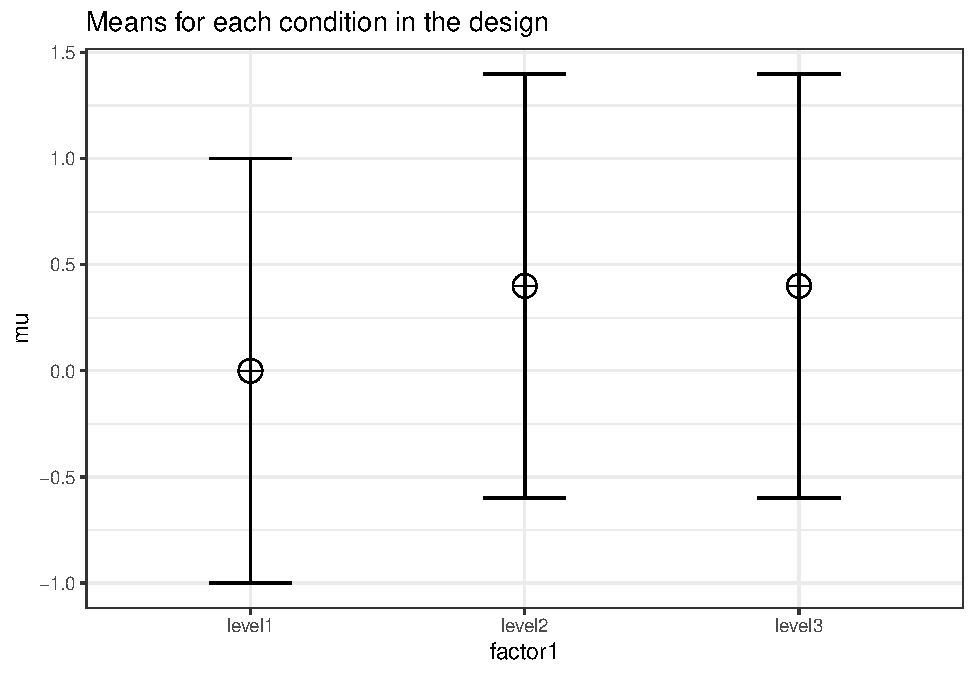
\includegraphics{SuperpowerValidation_files/figure-latex/unnamed-chunk-26-1.pdf}

\begin{Shaded}
\begin{Highlighting}[]
\KeywordTok{ANOVA_power}\NormalTok{(design_result, }\DataTypeTok{nsims =}\NormalTok{ nsims)}
\end{Highlighting}
\end{Shaded}

\begin{verbatim}
## Power and Effect sizes for ANOVA tests
##               power effect_size
## anova_factor1    81     0.04089
## 
## Power and Effect sizes for contrasts
##                                 power effect_size
## p_factor1_level1_factor1_level2    82     0.40691
## p_factor1_level1_factor1_level3    75     0.39780
## p_factor1_level2_factor1_level3     3    -0.01002
\end{verbatim}

\hypertarget{variation-1}{%
\section{Variation 1}\label{variation-1}}

\begin{Shaded}
\begin{Highlighting}[]
\CommentTok{# give sample sizes (all samples sizes are equal)}
\NormalTok{N =}\StringTok{ }\DecValTok{145}
\CommentTok{# give effect size d}
\NormalTok{d1 =}\StringTok{ }\FloatTok{.4} \CommentTok{#difference between the extremes}
\NormalTok{d2 =}\StringTok{ }\FloatTok{.0} \CommentTok{#third condition goes with the highest extreme}
\CommentTok{# give number of simulations}
\NormalTok{nSim =}\StringTok{ }\NormalTok{nsims}
\CommentTok{# give alpha levels}
\NormalTok{alpha1 =}\StringTok{ }\FloatTok{.05} \CommentTok{#alpha level for the omnibus ANOVA}
\NormalTok{alpha2 =}\StringTok{ }\FloatTok{.05} \CommentTok{#alpha level for three post hoc one-tailed t-tests Bonferroni correction}
\CommentTok{# create progress bar in case it takes a while}
\CommentTok{#pb <- winProgressBar(title = "progress bar", min = 0, max = nSim, width = 300)}
\CommentTok{# create vectors to store p-values}
\NormalTok{p1 <-}\KeywordTok{numeric}\NormalTok{(nSim) }\CommentTok{#p-value omnibus ANOVA}
\NormalTok{p2 <-}\KeywordTok{numeric}\NormalTok{(nSim) }\CommentTok{#p-value first post hoc test}
\NormalTok{p3 <-}\KeywordTok{numeric}\NormalTok{(nSim) }\CommentTok{#p-value second post hoc test}
\NormalTok{p4 <-}\KeywordTok{numeric}\NormalTok{(nSim) }\CommentTok{#p-value third post hoc test}
\NormalTok{pes1 <-}\KeywordTok{numeric}\NormalTok{(nSim) }\CommentTok{#partial eta-squared}
\NormalTok{pes2 <-}\KeywordTok{numeric}\NormalTok{(nSim) }\CommentTok{#partial eta-squared two extreme conditions}
\KeywordTok{library}\NormalTok{(lsr)}
\ControlFlowTok{for}\NormalTok{(i }\ControlFlowTok{in} \DecValTok{1}\OperatorTok{:}\NormalTok{nSim)\{ }\CommentTok{#for each simulated experiment}
 \CommentTok{# setWinProgressBar(pb, i, title=paste(round(i/nSim*100, 1), "% done"))}
\NormalTok{  x<-}\KeywordTok{rnorm}\NormalTok{(}\DataTypeTok{n =}\NormalTok{ N, }\DataTypeTok{mean =} \DecValTok{0}\NormalTok{, }\DataTypeTok{sd =} \DecValTok{1}\NormalTok{)}
\NormalTok{  y<-}\KeywordTok{rnorm}\NormalTok{(}\DataTypeTok{n =}\NormalTok{ N, }\DataTypeTok{mean =}\NormalTok{ d1, }\DataTypeTok{sd =} \DecValTok{1}\NormalTok{) }
\NormalTok{  z<-}\KeywordTok{rnorm}\NormalTok{(}\DataTypeTok{n =}\NormalTok{ N, }\DataTypeTok{mean =}\NormalTok{ d2, }\DataTypeTok{sd =} \DecValTok{1}\NormalTok{) }
\NormalTok{  data =}\StringTok{ }\KeywordTok{c}\NormalTok{(x,y,z)}
\NormalTok{  groups=}\StringTok{ }\KeywordTok{factor}\NormalTok{(}\KeywordTok{rep}\NormalTok{(letters[}\DecValTok{24}\OperatorTok{:}\DecValTok{26}\NormalTok{], }\DataTypeTok{each =}\NormalTok{ N))}
\NormalTok{  test <-}\StringTok{ }\KeywordTok{aov}\NormalTok{(data}\OperatorTok{~}\NormalTok{groups)}
\NormalTok{  pes1[i] <-}\StringTok{ }\KeywordTok{etaSquared}\NormalTok{(test)[}\DecValTok{1}\NormalTok{,}\DecValTok{2}\NormalTok{]}
\NormalTok{  p1[i] <-}\StringTok{ }\KeywordTok{summary}\NormalTok{(test)[[}\DecValTok{1}\NormalTok{]][[}\StringTok{"Pr(>F)"}\NormalTok{]][[}\DecValTok{1}\NormalTok{]]}
\NormalTok{  p2[i] <-}\StringTok{ }\KeywordTok{t.test}\NormalTok{(x,y)}\OperatorTok{$}\NormalTok{p.value}
\NormalTok{  p3[i] <-}\StringTok{ }\KeywordTok{t.test}\NormalTok{(x,z)}\OperatorTok{$}\NormalTok{p.value}
\NormalTok{  p4[i] <-}\StringTok{ }\KeywordTok{t.test}\NormalTok{(y,z)}\OperatorTok{$}\NormalTok{p.value}
\NormalTok{  data =}\StringTok{ }\KeywordTok{c}\NormalTok{(x,y)}
\NormalTok{  groups=}\StringTok{ }\KeywordTok{factor}\NormalTok{(}\KeywordTok{rep}\NormalTok{(letters[}\DecValTok{24}\OperatorTok{:}\DecValTok{25}\NormalTok{], }\DataTypeTok{each =}\NormalTok{ N))}
\NormalTok{  test <-}\StringTok{ }\KeywordTok{aov}\NormalTok{(data}\OperatorTok{~}\NormalTok{groups)}
\NormalTok{  pes2[i] <-}\StringTok{ }\KeywordTok{etaSquared}\NormalTok{(test)[}\DecValTok{1}\NormalTok{,}\DecValTok{2}\NormalTok{]}
\NormalTok{  \}}
\CommentTok{#close(pb)#close progress bar}
\CommentTok{# results are as predicted when omnibus ANOVA is significant, t-tests are significant between x and y plus x and z; not significant between y and z}
\CommentTok{#printing all unique tests (adjusted code by DL)}
\KeywordTok{sum}\NormalTok{(p1}\OperatorTok{<}\NormalTok{alpha1)}\OperatorTok{/}\NormalTok{nSim}
\end{Highlighting}
\end{Shaded}

\begin{verbatim}
## [1] 0.9
\end{verbatim}

\begin{Shaded}
\begin{Highlighting}[]
\KeywordTok{sum}\NormalTok{(p2}\OperatorTok{<}\NormalTok{alpha2)}\OperatorTok{/}\NormalTok{nSim}
\end{Highlighting}
\end{Shaded}

\begin{verbatim}
## [1] 0.91
\end{verbatim}

\begin{Shaded}
\begin{Highlighting}[]
\KeywordTok{sum}\NormalTok{(p3}\OperatorTok{<}\NormalTok{alpha2)}\OperatorTok{/}\NormalTok{nSim}
\end{Highlighting}
\end{Shaded}

\begin{verbatim}
## [1] 0.03
\end{verbatim}

\begin{Shaded}
\begin{Highlighting}[]
\KeywordTok{sum}\NormalTok{(p4}\OperatorTok{<}\NormalTok{alpha2)}\OperatorTok{/}\NormalTok{nSim}
\end{Highlighting}
\end{Shaded}

\begin{verbatim}
## [1] 0.91
\end{verbatim}

\begin{Shaded}
\begin{Highlighting}[]
\KeywordTok{mean}\NormalTok{(pes1)}
\end{Highlighting}
\end{Shaded}

\begin{verbatim}
## [1] 0.03644733
\end{verbatim}

\begin{Shaded}
\begin{Highlighting}[]
\KeywordTok{mean}\NormalTok{(pes2)}
\end{Highlighting}
\end{Shaded}

\begin{verbatim}
## [1] 0.04017308
\end{verbatim}

\hypertarget{three-conditions-replication-1}{%
\section{Three conditions replication}\label{three-conditions-replication-1}}

\begin{Shaded}
\begin{Highlighting}[]
\NormalTok{K <-}\StringTok{ }\DecValTok{3}
\NormalTok{mu <-}\StringTok{ }\KeywordTok{c}\NormalTok{(}\DecValTok{0}\NormalTok{, }\FloatTok{0.4}\NormalTok{, }\FloatTok{0.0}\NormalTok{)}
\NormalTok{n <-}\StringTok{ }\DecValTok{145}
\NormalTok{sd <-}\StringTok{ }\DecValTok{1}
\NormalTok{r <-}\StringTok{ }\DecValTok{0}
\NormalTok{design =}\KeywordTok{paste}\NormalTok{(K,}\StringTok{"b"}\NormalTok{,}\DataTypeTok{sep=}\StringTok{""}\NormalTok{)}
\end{Highlighting}
\end{Shaded}

\begin{Shaded}
\begin{Highlighting}[]
\NormalTok{design_result <-}\StringTok{ }\KeywordTok{ANOVA_design}\NormalTok{(}\DataTypeTok{design =}\NormalTok{string,}
                   \DataTypeTok{n =}\NormalTok{ n, }
                   \DataTypeTok{mu =}\NormalTok{ mu, }
                   \DataTypeTok{sd =}\NormalTok{ sd, }
                   \DataTypeTok{labelnames =} \KeywordTok{c}\NormalTok{(}\StringTok{"factor1"}\NormalTok{, }\StringTok{"level1"}\NormalTok{, }\StringTok{"level2"}\NormalTok{, }\StringTok{"level3"}\NormalTok{))}
\end{Highlighting}
\end{Shaded}

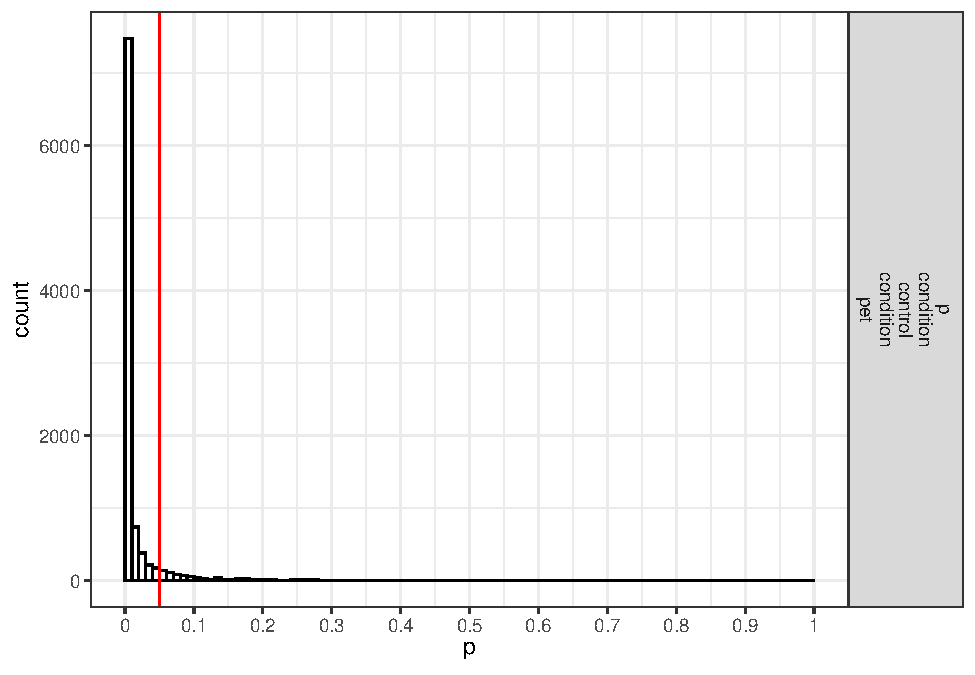
\includegraphics{SuperpowerValidation_files/figure-latex/unnamed-chunk-29-1.pdf}

\begin{Shaded}
\begin{Highlighting}[]
\KeywordTok{ANOVA_power}\NormalTok{(design_result, }\DataTypeTok{nsims =}\NormalTok{ nsims)}
\end{Highlighting}
\end{Shaded}

\begin{verbatim}
## Power and Effect sizes for ANOVA tests
##               power effect_size
## anova_factor1    92     0.03871
## 
## Power and Effect sizes for contrasts
##                                 power effect_size
## p_factor1_level1_factor1_level2    91    0.397884
## p_factor1_level1_factor1_level3     5   -0.005665
## p_factor1_level2_factor1_level3    91   -0.403446
\end{verbatim}

\hypertarget{variation-2}{%
\section{Variation 2}\label{variation-2}}

\begin{Shaded}
\begin{Highlighting}[]
\CommentTok{# give sample sizes (all samples sizes are equal)}
\NormalTok{N =}\StringTok{ }\DecValTok{82}
\CommentTok{# give effect size d}
\NormalTok{d1 =}\StringTok{ }\FloatTok{.4} \CommentTok{#difference between the extremes}
\NormalTok{d2 =}\StringTok{ }\FloatTok{.2} \CommentTok{#third condition goes with the highest extreme}
\CommentTok{# give number of simulations}
\NormalTok{nSim =}\StringTok{ }\NormalTok{nsims}
\CommentTok{# give alpha levels}
\NormalTok{alpha1 =}\StringTok{ }\FloatTok{.05} \CommentTok{#alpha level for the omnibus ANOVA}
\NormalTok{alpha2 =}\StringTok{ }\FloatTok{.05} \CommentTok{#alpha level for three post hoc one-tailed t-tests Bonferroni correction}
\CommentTok{# create progress bar in case it takes a while}
\CommentTok{#pb <- winProgressBar(title = "progress bar", min = 0, max = nSim, width = 300)}
\CommentTok{# create vectors to store p-values}
\NormalTok{p1 <-}\KeywordTok{numeric}\NormalTok{(nSim) }\CommentTok{#p-value omnibus ANOVA}
\NormalTok{p2 <-}\KeywordTok{numeric}\NormalTok{(nSim) }\CommentTok{#p-value first post hoc test}
\NormalTok{p3 <-}\KeywordTok{numeric}\NormalTok{(nSim) }\CommentTok{#p-value second post hoc test}
\NormalTok{p4 <-}\KeywordTok{numeric}\NormalTok{(nSim) }\CommentTok{#p-value third post hoc test}
\NormalTok{pes1 <-}\KeywordTok{numeric}\NormalTok{(nSim) }\CommentTok{#partial eta-squared}
\NormalTok{pes2 <-}\KeywordTok{numeric}\NormalTok{(nSim) }\CommentTok{#partial eta-squared two extreme conditions}
\KeywordTok{library}\NormalTok{(lsr)}
\ControlFlowTok{for}\NormalTok{(i }\ControlFlowTok{in} \DecValTok{1}\OperatorTok{:}\NormalTok{nSim)\{ }\CommentTok{#for each simulated experiment}
 \CommentTok{# setWinProgressBar(pb, i, title=paste(round(i/nSim*100, 1), "% done"))}
\NormalTok{  x<-}\KeywordTok{rnorm}\NormalTok{(}\DataTypeTok{n =}\NormalTok{ N, }\DataTypeTok{mean =} \DecValTok{0}\NormalTok{, }\DataTypeTok{sd =} \DecValTok{1}\NormalTok{)}
\NormalTok{  y<-}\KeywordTok{rnorm}\NormalTok{(}\DataTypeTok{n =}\NormalTok{ N, }\DataTypeTok{mean =}\NormalTok{ d1, }\DataTypeTok{sd =} \DecValTok{1}\NormalTok{) }
\NormalTok{  z<-}\KeywordTok{rnorm}\NormalTok{(}\DataTypeTok{n =}\NormalTok{ N, }\DataTypeTok{mean =}\NormalTok{ d2, }\DataTypeTok{sd =} \DecValTok{1}\NormalTok{) }
\NormalTok{  data =}\StringTok{ }\KeywordTok{c}\NormalTok{(x,y,z)}
\NormalTok{  groups=}\StringTok{ }\KeywordTok{factor}\NormalTok{(}\KeywordTok{rep}\NormalTok{(letters[}\DecValTok{24}\OperatorTok{:}\DecValTok{26}\NormalTok{], }\DataTypeTok{each =}\NormalTok{ N))}
\NormalTok{  test <-}\StringTok{ }\KeywordTok{aov}\NormalTok{(data}\OperatorTok{~}\NormalTok{groups)}
\NormalTok{  pes1[i] <-}\StringTok{ }\KeywordTok{etaSquared}\NormalTok{(test)[}\DecValTok{1}\NormalTok{,}\DecValTok{2}\NormalTok{]}
\NormalTok{  p1[i] <-}\StringTok{ }\KeywordTok{summary}\NormalTok{(test)[[}\DecValTok{1}\NormalTok{]][[}\StringTok{"Pr(>F)"}\NormalTok{]][[}\DecValTok{1}\NormalTok{]]}
\NormalTok{  p2[i] <-}\StringTok{ }\KeywordTok{t.test}\NormalTok{(x,y)}\OperatorTok{$}\NormalTok{p.value}
\NormalTok{  p3[i] <-}\StringTok{ }\KeywordTok{t.test}\NormalTok{(x,z)}\OperatorTok{$}\NormalTok{p.value}
\NormalTok{  p4[i] <-}\StringTok{ }\KeywordTok{t.test}\NormalTok{(y,z)}\OperatorTok{$}\NormalTok{p.value}
\NormalTok{  data =}\StringTok{ }\KeywordTok{c}\NormalTok{(x,y)}
\NormalTok{  groups=}\StringTok{ }\KeywordTok{factor}\NormalTok{(}\KeywordTok{rep}\NormalTok{(letters[}\DecValTok{24}\OperatorTok{:}\DecValTok{25}\NormalTok{], }\DataTypeTok{each =}\NormalTok{ N))}
\NormalTok{  test <-}\StringTok{ }\KeywordTok{aov}\NormalTok{(data}\OperatorTok{~}\NormalTok{groups)}
\NormalTok{  pes2[i] <-}\StringTok{ }\KeywordTok{etaSquared}\NormalTok{(test)[}\DecValTok{1}\NormalTok{,}\DecValTok{2}\NormalTok{]}
\NormalTok{  \}}
\CommentTok{#close(pb)#close progress bar}
\CommentTok{# results are as predicted when omnibus ANOVA is significant, t-tests are significant between x and y plus x and z; not significant between y and z}
\CommentTok{#printing all unique tests (adjusted code by DL)}
\KeywordTok{sum}\NormalTok{(p1}\OperatorTok{<}\NormalTok{alpha1)}\OperatorTok{/}\NormalTok{nSim}
\end{Highlighting}
\end{Shaded}

\begin{verbatim}
## [1] 0.58
\end{verbatim}

\begin{Shaded}
\begin{Highlighting}[]
\KeywordTok{sum}\NormalTok{(p2}\OperatorTok{<}\NormalTok{alpha2)}\OperatorTok{/}\NormalTok{nSim}
\end{Highlighting}
\end{Shaded}

\begin{verbatim}
## [1] 0.62
\end{verbatim}

\begin{Shaded}
\begin{Highlighting}[]
\KeywordTok{sum}\NormalTok{(p3}\OperatorTok{<}\NormalTok{alpha2)}\OperatorTok{/}\NormalTok{nSim}
\end{Highlighting}
\end{Shaded}

\begin{verbatim}
## [1] 0.26
\end{verbatim}

\begin{Shaded}
\begin{Highlighting}[]
\KeywordTok{sum}\NormalTok{(p4}\OperatorTok{<}\NormalTok{alpha2)}\OperatorTok{/}\NormalTok{nSim}
\end{Highlighting}
\end{Shaded}

\begin{verbatim}
## [1] 0.2
\end{verbatim}

\begin{Shaded}
\begin{Highlighting}[]
\KeywordTok{mean}\NormalTok{(pes1)}
\end{Highlighting}
\end{Shaded}

\begin{verbatim}
## [1] 0.03198582
\end{verbatim}

\begin{Shaded}
\begin{Highlighting}[]
\KeywordTok{mean}\NormalTok{(pes2)}
\end{Highlighting}
\end{Shaded}

\begin{verbatim}
## [1] 0.04184699
\end{verbatim}

\hypertarget{three-conditions-replication-2}{%
\section{Three conditions replication}\label{three-conditions-replication-2}}

\begin{Shaded}
\begin{Highlighting}[]
\NormalTok{K <-}\StringTok{ }\DecValTok{3}
\NormalTok{mu <-}\StringTok{ }\KeywordTok{c}\NormalTok{(}\DecValTok{0}\NormalTok{, }\FloatTok{0.4}\NormalTok{, }\FloatTok{0.2}\NormalTok{)}
\NormalTok{n <-}\StringTok{ }\DecValTok{82}
\NormalTok{sd <-}\StringTok{ }\DecValTok{1}
\NormalTok{design =}\KeywordTok{paste}\NormalTok{(K,}\StringTok{"b"}\NormalTok{,}\DataTypeTok{sep=}\StringTok{""}\NormalTok{)}
\end{Highlighting}
\end{Shaded}

\begin{Shaded}
\begin{Highlighting}[]
\NormalTok{design_result <-}\StringTok{ }\KeywordTok{ANOVA_design}\NormalTok{(}\DataTypeTok{design =}\NormalTok{string,}
                   \DataTypeTok{n =}\NormalTok{ n, }
                   \DataTypeTok{mu =}\NormalTok{ mu, }
                   \DataTypeTok{sd =}\NormalTok{ sd, }
                   \DataTypeTok{labelnames =} \KeywordTok{c}\NormalTok{(}\StringTok{"factor1"}\NormalTok{, }\StringTok{"level1"}\NormalTok{, }\StringTok{"level2"}\NormalTok{, }\StringTok{"level3"}\NormalTok{))}
\end{Highlighting}
\end{Shaded}

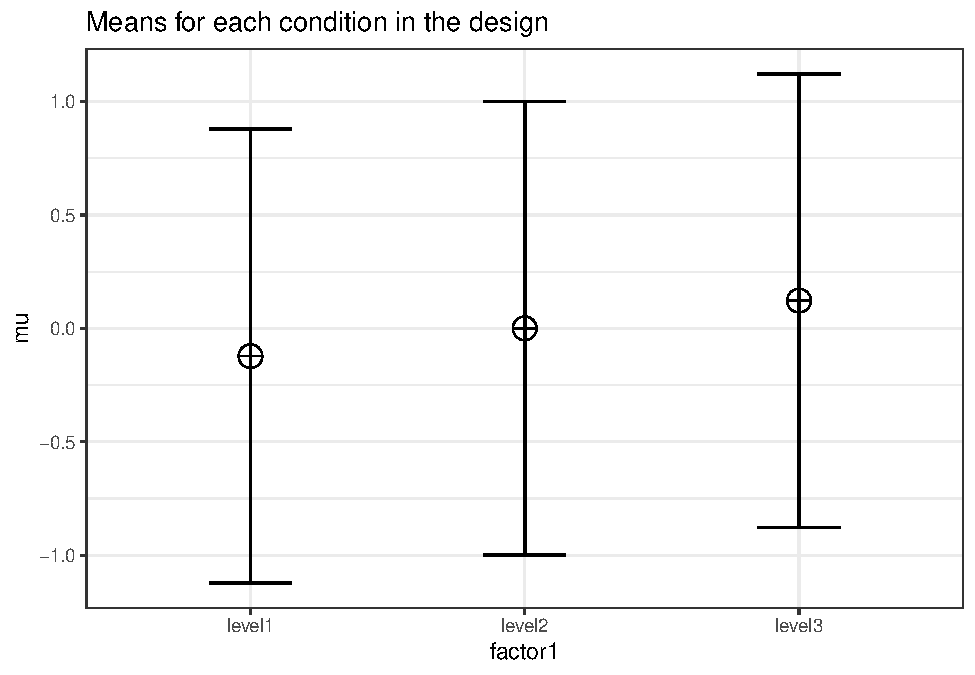
\includegraphics{SuperpowerValidation_files/figure-latex/unnamed-chunk-32-1.pdf}

\begin{Shaded}
\begin{Highlighting}[]
\KeywordTok{ANOVA_power}\NormalTok{(design_result, }\DataTypeTok{nsims =}\NormalTok{ nsims)}
\end{Highlighting}
\end{Shaded}

\begin{verbatim}
## Power and Effect sizes for ANOVA tests
##               power effect_size
## anova_factor1    58     0.03266
## 
## Power and Effect sizes for contrasts
##                                 power effect_size
## p_factor1_level1_factor1_level2    71      0.3891
## p_factor1_level1_factor1_level3    24      0.1995
## p_factor1_level2_factor1_level3    20     -0.1892
\end{verbatim}

\hypertarget{repeated-measures-anova-part-1}{%
\chapter{Repeated Measures-ANOVA Part 1}\label{repeated-measures-anova-part-1}}

In a repeated measures design multiple observations are collected from the same participants. In the simplest case, where there are two repeated observations, a repeated measures ANOVA equals a dependent or paired \emph{t}-test. The difference compared to a between subject design is that repeated measures can be correlated, and in psychology, they often are. Let's first explore the impact of this correlation on the power of a repeated measures ANOVA.

\hypertarget{two-conditions-medium-effect-size}{%
\section{Two conditions, medium effect size}\label{two-conditions-medium-effect-size}}

To illustrate the effect of correated observations, we start by simulating data for a medium effect size for a dependent (or paired, or within-subject) \emph{t}-test. Let's first look at G*power. If we want to perform an a-priori power analysis, we are asked to fill in the effect size dz. As Cohen (1988) writes, ``The Z subscript is used to emphasize the fact that our raw score unit is no longer X or Y, but Z'', where Z are the difference scores of X-Y.

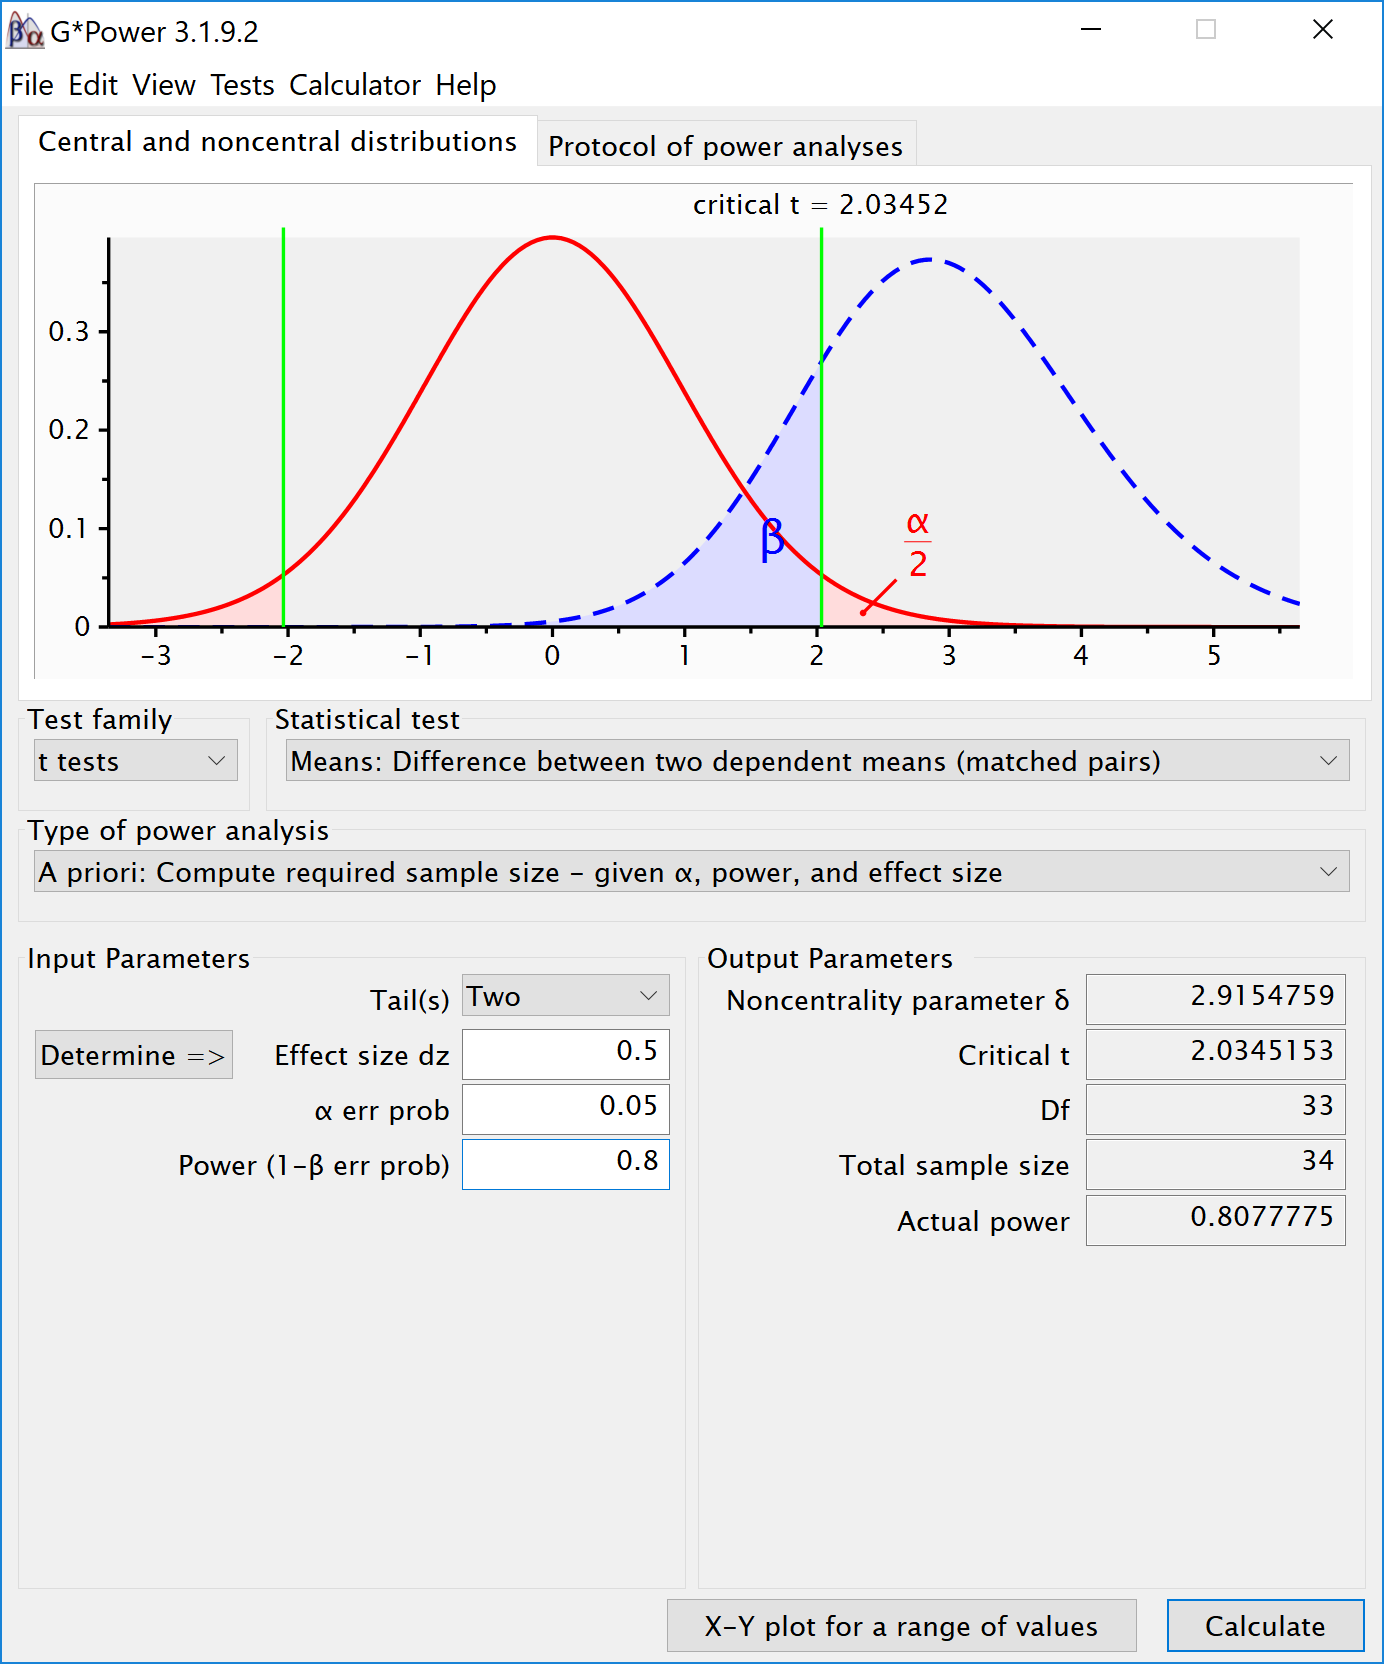
\includegraphics{screenshots/gpower_9.png}

Within designs can have greater power to detect differences than between designs because the values are correlated, and a within design requires less participants because each participant provides multiple observations. One difference between an independent \emph{t}-test and a dependent \emph{t}-test is that an independent \emph{t}-test has 2(n-1) degrees of freedom, while a dependent \emph{t}-test has (n-1) degrees of freedom. The sample size needed in a two-group within-design (NW) relative to the sample needed in two-group between-designs (NB), assuming normal distributions, and ignoring the difference in degrees of freedom between the two types of tests, is (from Maxwell \& Delaney, 2004, p.~561, formula 45):

\(N_{W}=\frac{N_{B}(1-\rho)}{2}\)

The division by 2 in the equation is due to the fact that in a two-condition within design every participant provides two data-points. The extent to which this reduces the sample size compared to a between-subject design depends on the correlation (\emph{r}) between the two dependent variables, as indicated by the 1-r part of the equation. If the correlation is 0, a within-subject design needs half as many participants as a between-subject design (e.g., 64 instead 128 participants), simply because every participants provides 2 datapoints. The higher the correlation, the larger the relative benefit of within designs, and whenever the correlation is negative (up to -1) the relative benefit disappears.

Whereas in an independent \emph{t}-test the two observations are uncorrelated, in a within design the observations are correlated. This has an effect on the standard deviation of the difference scores. In turn, because the standardized effect size is the mean difference divided by the standard deviation of the difference scores, the correlation has an effect on the standardized mean difference in a within design, Cohen's dz. The relation, as Cohen (1988, formula 2.3.7) explains, is:

\(\sigma_{z}=\sigma\sqrt{2(1-\rho)}\)

Therefore, the relation between dz and d is \(\sqrt{2(1-\rho)}\). As Cohen (1988) writes: "In other words, a given difference between population means for matched (dependent) samples is standardized by a value which is \(\sqrt{2(1-\rho)}\) as large as would be the case were they independent. If we enter a correlation of 0.5 in the formula, we get \(\sqrt{2(0.5)}=1\). In other words, when the correlation is 0.5, d = dz. When there is a strong correlation between dependent variables, for example r = 0.9, we get \(d=d_{z}\sqrt{2(1-0.9)}\), and a dz of 1 would be a d = 0.45. Reversely, \(d_{z}=\frac{d}{\sqrt{2(1-r)}}\), so with a r = 0.9, a d of 1 would be a dz = 2.24. Some consider this increase in dz compared to d when observations are strongly correlated an `inflation' when estimating effect sizes, but since the reduction in the standard deviation of the difference scores due to the correlation makes it easier to distinguish signal from noise in a hypothesis test, it leads to a clear power benefit.

\begin{Shaded}
\begin{Highlighting}[]
\CommentTok{# Check sample size formula Maxwell}
\CommentTok{# Power is pretty similar with n/2, same d (assuming r = 0.5). }
\CommentTok{# Small differences due to df = 2(n-1) vs df = n-1}
\KeywordTok{pwr.t.test}\NormalTok{(}\DataTypeTok{d =} \FloatTok{0.05}\NormalTok{,}
           \DataTypeTok{n =} \KeywordTok{c}\NormalTok{(}\DecValTok{2000}\NormalTok{, }\DecValTok{4000}\NormalTok{, }\DecValTok{8000}\NormalTok{),}
           \DataTypeTok{sig.level =} \FloatTok{0.05}\NormalTok{,}
           \DataTypeTok{type =} \StringTok{"two.sample"}\NormalTok{,}
           \DataTypeTok{alternative =} \StringTok{"two.sided"}\NormalTok{)}
\end{Highlighting}
\end{Shaded}

\begin{verbatim}
## 
##      Two-sample t test power calculation 
## 
##               n = 2000, 4000, 8000
##               d = 0.05
##       sig.level = 0.05
##           power = 0.3524674, 0.6086764, 0.8853424
##     alternative = two.sided
## 
## NOTE: n is number in *each* group
\end{verbatim}

\begin{Shaded}
\begin{Highlighting}[]
\KeywordTok{pwr.t.test}\NormalTok{(}\DataTypeTok{d =} \FloatTok{0.05}\NormalTok{,}
           \DataTypeTok{n =} \KeywordTok{c}\NormalTok{(}\DecValTok{1000}\NormalTok{, }\DecValTok{2000}\NormalTok{, }\DecValTok{4000}\NormalTok{),}
           \DataTypeTok{sig.level =} \FloatTok{0.05}\NormalTok{,}
           \DataTypeTok{type =} \StringTok{"paired"}\NormalTok{,}
           \DataTypeTok{alternative =} \StringTok{"two.sided"}\NormalTok{)}
\end{Highlighting}
\end{Shaded}

\begin{verbatim}
## 
##      Paired t test power calculation 
## 
##               n = 1000, 2000, 4000
##               d = 0.05
##       sig.level = 0.05
##           power = 0.3520450, 0.6083669, 0.8852320
##     alternative = two.sided
## 
## NOTE: n is number of *pairs*
\end{verbatim}

There is no equivalent fz for Cohen's f for a within subject ANOVA. For two groups, we can directly compute Cohen's f from Cohen's d for two groups, as Cohen (1988) describes, because f = 1/2d. For a d = 0.5, f = 0.25. In Gpower we can run a 2 group within-subject power analysis for ANOVA. We plan for 80\% power, and reproduce the anaysis above for the dependent \emph{t}-test. This works because the correlation is set to 0.5, when d = dz, and thus the transformation of f=1/2d works.

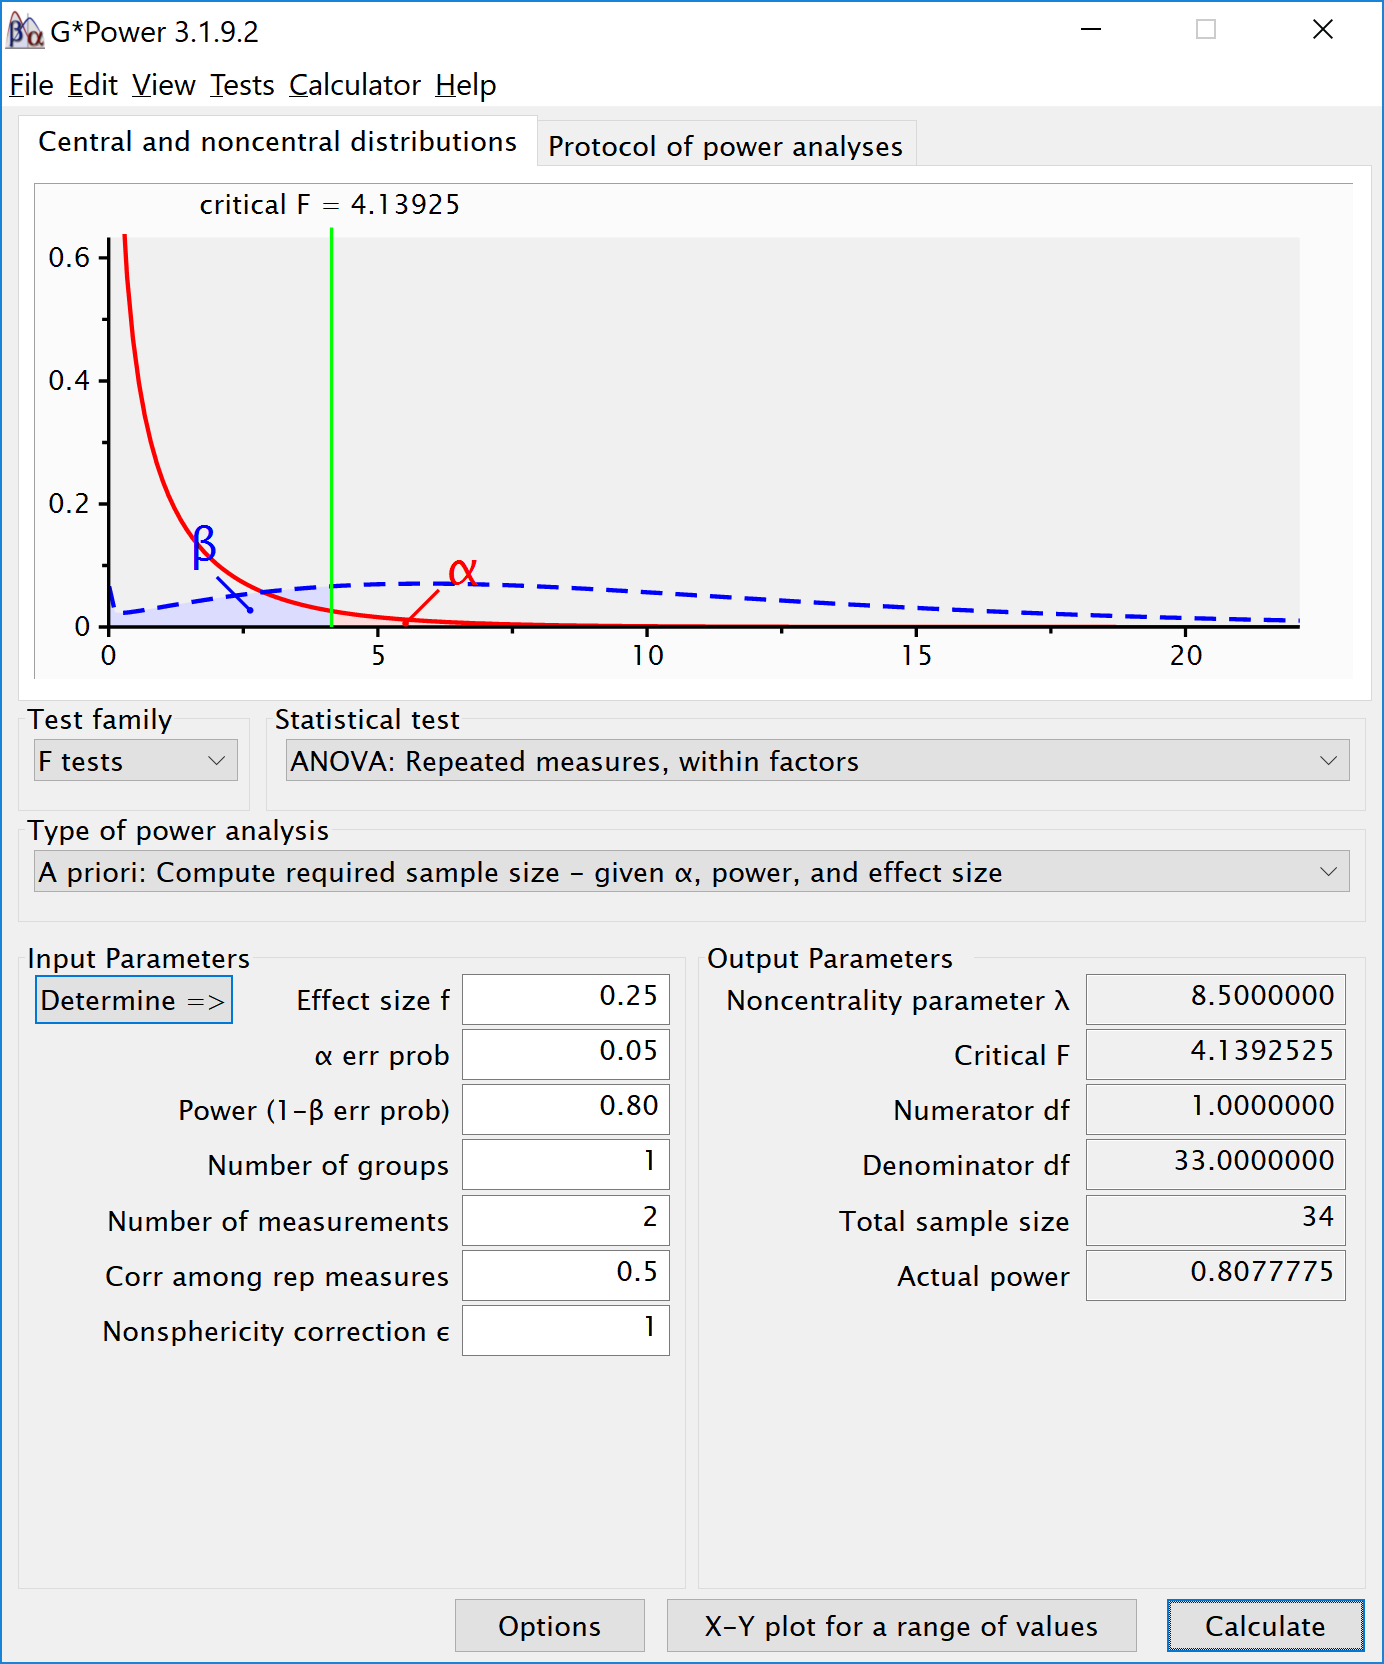
\includegraphics{screenshots/gpower_1.png}

If we change the correlation to 0.7 and keep all other settings the same, the repeated measure a-priori power analysis yields a sample of 21. The correlation increases the power for the test.

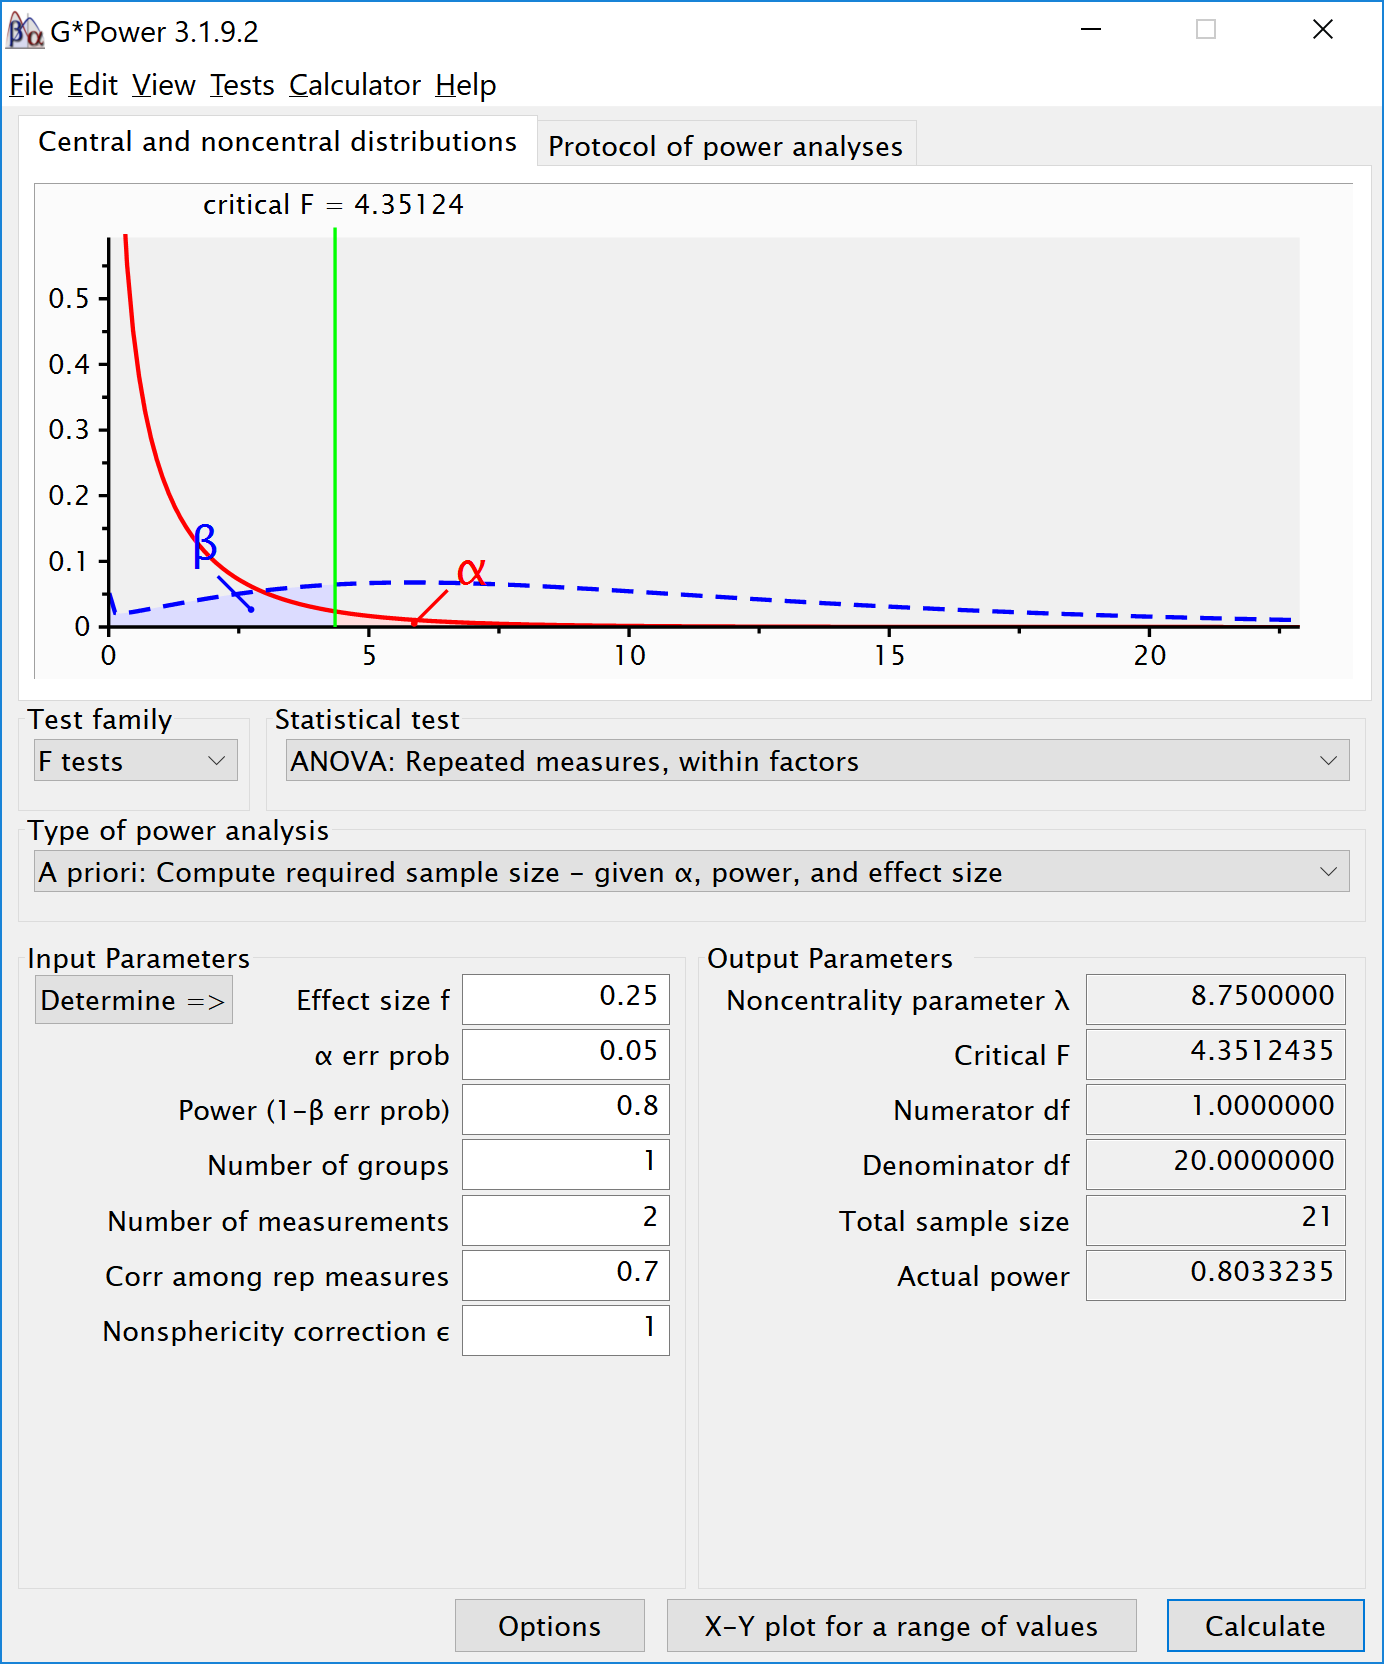
\includegraphics{screenshots/gpower_11.png}

To reproduce this analysis in Gpower with a dependent \emph{t}-test we need to change dz following the formula above, \(d_{z}=\frac{0.5}{\sqrt{2(1-0.7)}}\), which yields dz = 0.6454972. If we enter this value in Gpower for an a-priori power analysis, we get the exact same results (as we should, since an repeated measures ANOVA with 2 groups equals a dependent \emph{t}-test). This example illustrates that the correlation between dependent variables always factors into a power analysis, both for a dependent \emph{t}-test, and for a repeated measures ANOVA. Because a dependent \emph{t}-test uses dz the correlation might be less visible, but given the relation between d and dz, the correlation is always taken into account and can greatly improve power for within designs compared to between designs.

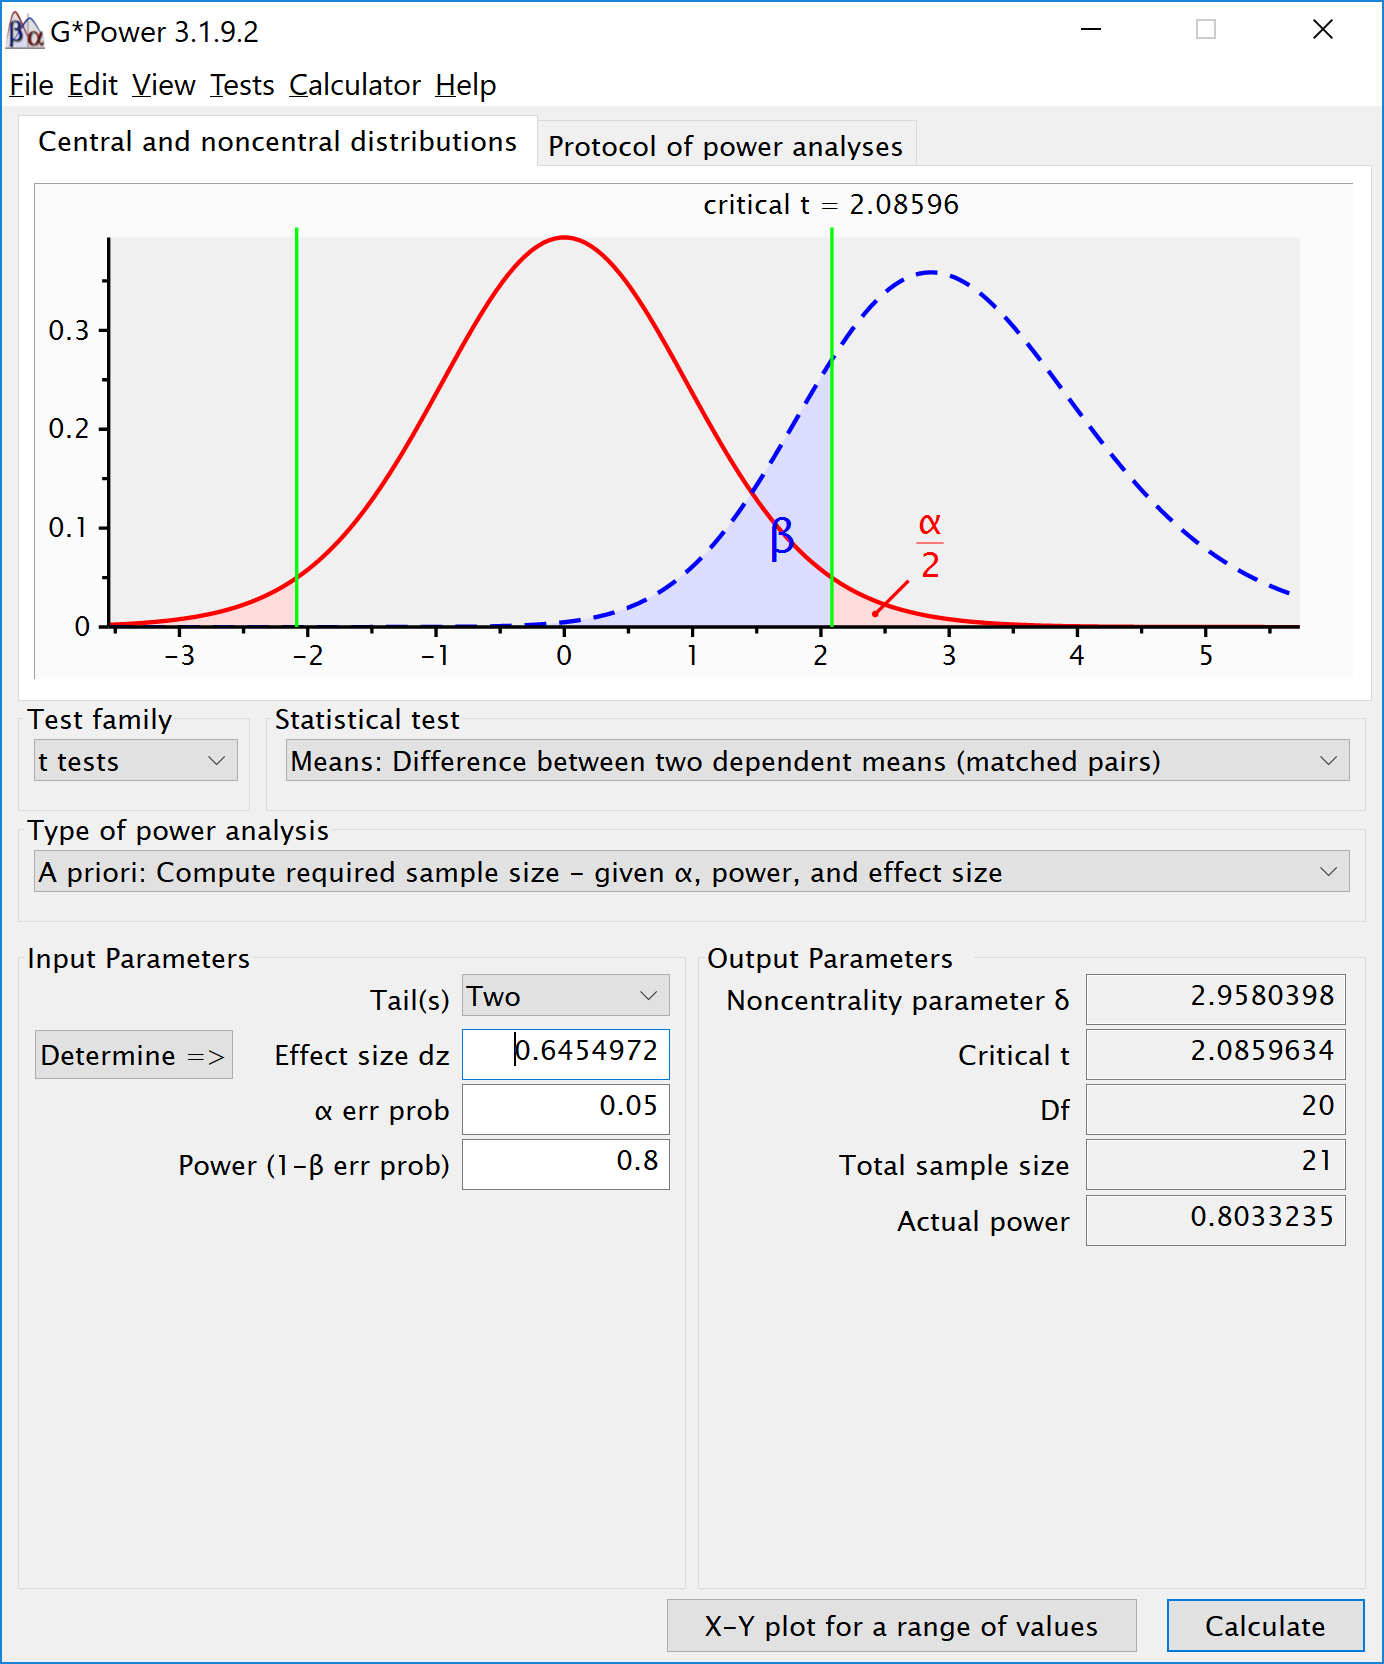
\includegraphics{screenshots/gpower_10.png}

We can perform both these power analyses using simuations as well. We set groups to 2 for the simulation, n = 34 (which should give 80.777 power, according to the g*power program), a correlation among repeated measures of 0.5, and an alpha of 0.05. In this case, we simulate data with means -0.25 and 0.25, and set the sd to 1. This means we have a mean difference of 0.5, and a Cohen's d of 0.5/1 = 0.5. In the first example, we set the correlation to 0.5, and the result should be 80.77\% power, and an effect size estimate of 0.5 for the simple effect. We also calculate partial eta-squared for the ANOVA, which equals \(\frac{f^2}{f^2+1}\), or 0.05882353.

\begin{Shaded}
\begin{Highlighting}[]
\NormalTok{K <-}\StringTok{ }\DecValTok{2}
\NormalTok{n <-}\StringTok{ }\DecValTok{34}
\NormalTok{sd <-}\StringTok{ }\DecValTok{1}
\NormalTok{r <-}\StringTok{ }\FloatTok{0.5}
\NormalTok{alpha =}\StringTok{ }\FloatTok{0.05}
\NormalTok{f <-}\StringTok{ }\FloatTok{0.25}
\NormalTok{f2 <-}\StringTok{ }\NormalTok{f}\OperatorTok{^}\DecValTok{2}
\NormalTok{ES <-}\StringTok{ }\NormalTok{f2}\OperatorTok{/}\NormalTok{(f2}\OperatorTok{+}\DecValTok{1}\NormalTok{)}
\NormalTok{ES}
\end{Highlighting}
\end{Shaded}

\begin{verbatim}
## [1] 0.05882353
\end{verbatim}

\begin{Shaded}
\begin{Highlighting}[]
\NormalTok{mu <-}\StringTok{ }\KeywordTok{mu_from_ES}\NormalTok{(}\DataTypeTok{K =}\NormalTok{ K, }\DataTypeTok{ES =}\NormalTok{ ES)}
\NormalTok{design =}\KeywordTok{paste}\NormalTok{(K,}\StringTok{"w"}\NormalTok{,}\DataTypeTok{sep=}\StringTok{""}\NormalTok{)}
\NormalTok{labelnames <-}\StringTok{ }\KeywordTok{c}\NormalTok{(}\StringTok{"speed"}\NormalTok{, }\StringTok{"fast"}\NormalTok{, }\StringTok{"slow"}\NormalTok{)}
\NormalTok{design_result <-}\StringTok{ }\KeywordTok{ANOVA_design}\NormalTok{(}\DataTypeTok{design =}\NormalTok{ design,}
                   \DataTypeTok{n =}\NormalTok{ n, }
                   \DataTypeTok{mu =}\NormalTok{ mu, }
                   \DataTypeTok{sd =}\NormalTok{ sd, }
                   \DataTypeTok{r =}\NormalTok{ r, }
                   \DataTypeTok{labelnames =}\NormalTok{ labelnames)}
\end{Highlighting}
\end{Shaded}

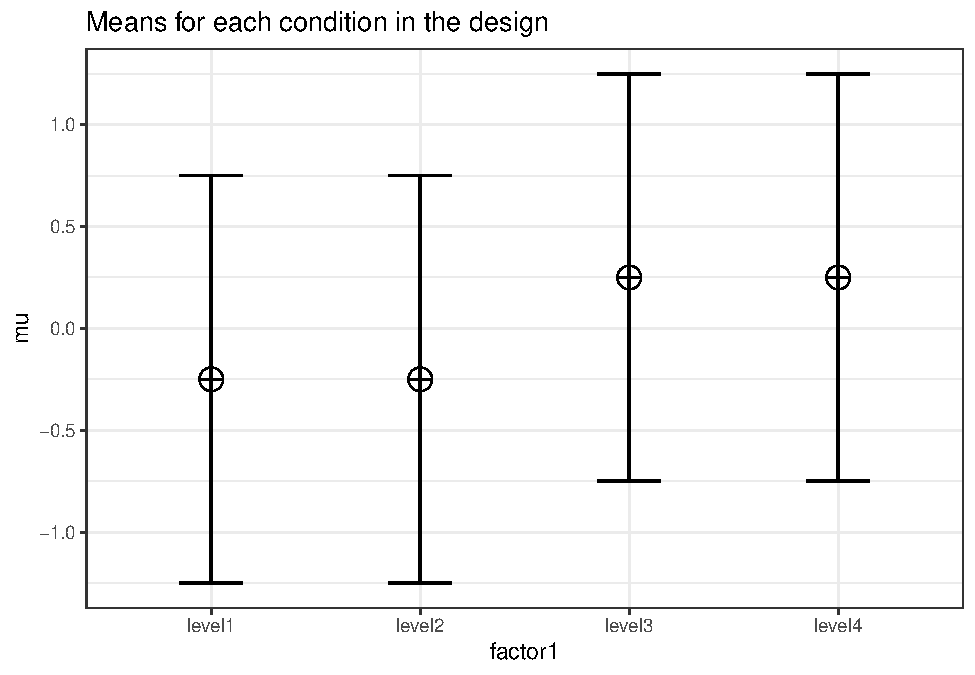
\includegraphics{SuperpowerValidation_files/figure-latex/unnamed-chunk-34-1.pdf}

\begin{Shaded}
\begin{Highlighting}[]
\NormalTok{alpha_level <-}\StringTok{ }\FloatTok{0.05}
\KeywordTok{ANOVA_power}\NormalTok{(design_result, }\DataTypeTok{nsims =}\NormalTok{ nsims)}
\end{Highlighting}
\end{Shaded}

\begin{verbatim}
## Power and Effect sizes for ANOVA tests
##             power effect_size
## anova_speed    83      0.2252
## 
## Power and Effect sizes for contrasts
##                         power effect_size
## p_speed_fast_speed_slow    83      0.5273
## 
## Within-Subject Factors Included: Check MANOVA Results
\end{verbatim}

The results of the simulation are indeed very close to 80.777\%. Note that the simulation calculates Cohen's dz effect sizes for paired comparisons - which here given the correlation of 0.5 is also 0.5 for a medium effect size.

We should see a larger dz if we increase the correlation, keeping the sample size the same, following the example in Gpower above. We repeat the simulation, and the only difference is a correlation between dependent variables of 0.7. This should yield an effect size dz = 0.6454972.

\begin{Shaded}
\begin{Highlighting}[]
\NormalTok{K <-}\StringTok{ }\DecValTok{2}
\NormalTok{n <-}\StringTok{ }\DecValTok{21}
\NormalTok{sd <-}\StringTok{ }\DecValTok{1}
\NormalTok{r <-}\StringTok{ }\FloatTok{0.7}
\NormalTok{alpha =}\StringTok{ }\FloatTok{0.05}
\NormalTok{f <-}\StringTok{ }\FloatTok{0.25}
\NormalTok{f2 <-}\StringTok{ }\NormalTok{f}\OperatorTok{^}\DecValTok{2}
\NormalTok{ES <-}\StringTok{ }\NormalTok{f2}\OperatorTok{/}\NormalTok{(f2}\OperatorTok{+}\DecValTok{1}\NormalTok{)}
\NormalTok{ES}
\end{Highlighting}
\end{Shaded}

\begin{verbatim}
## [1] 0.05882353
\end{verbatim}

\begin{Shaded}
\begin{Highlighting}[]
\NormalTok{mu <-}\StringTok{ }\KeywordTok{mu_from_ES}\NormalTok{(}\DataTypeTok{K =}\NormalTok{ K, }\DataTypeTok{ES =}\NormalTok{ ES)}
\NormalTok{design =}\StringTok{ }\KeywordTok{paste}\NormalTok{(K,}\StringTok{"w"}\NormalTok{,}\DataTypeTok{sep=}\StringTok{""}\NormalTok{)}
\NormalTok{labelnames <-}\StringTok{ }\KeywordTok{c}\NormalTok{(}\StringTok{"speed"}\NormalTok{, }\StringTok{"fast"}\NormalTok{, }\StringTok{"slow"}\NormalTok{)}
\NormalTok{design_result <-}\StringTok{ }\KeywordTok{ANOVA_design}\NormalTok{(}\DataTypeTok{design =}\NormalTok{ design,}
                   \DataTypeTok{n =}\NormalTok{ n, }
                   \DataTypeTok{mu =}\NormalTok{ mu, }
                   \DataTypeTok{sd =}\NormalTok{ sd, }
                   \DataTypeTok{r =}\NormalTok{ r, }
                   \DataTypeTok{labelnames =}\NormalTok{ labelnames)}
\end{Highlighting}
\end{Shaded}

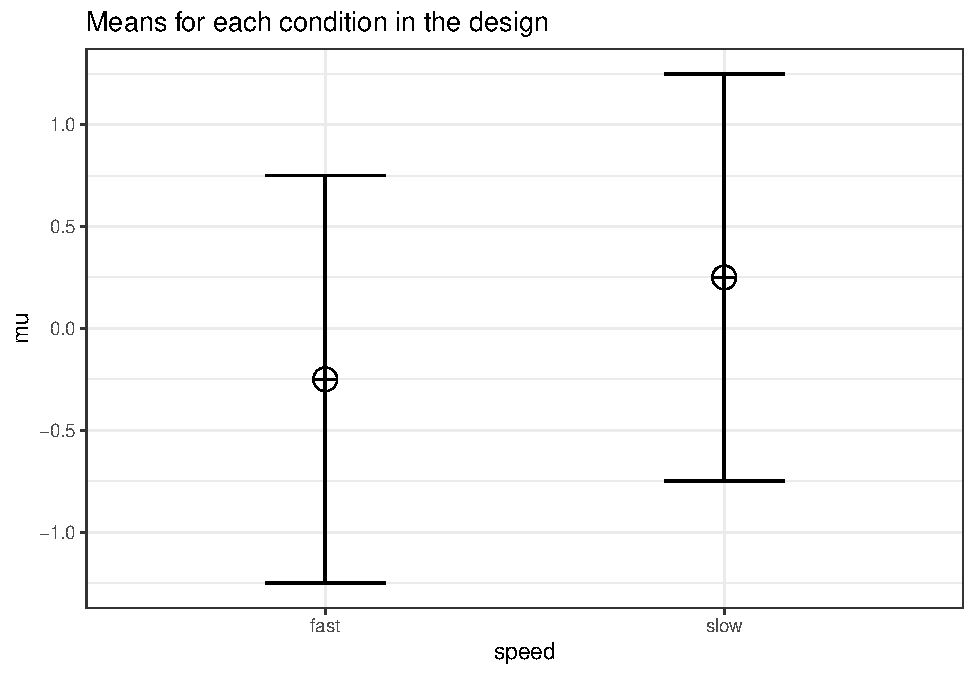
\includegraphics{SuperpowerValidation_files/figure-latex/unnamed-chunk-35-1.pdf}

\begin{Shaded}
\begin{Highlighting}[]
\NormalTok{alpha_level <-}\StringTok{ }\FloatTok{0.05}
\NormalTok{design_result}\OperatorTok{$}\NormalTok{sigmatrix}
\end{Highlighting}
\end{Shaded}

\begin{verbatim}
##      fast slow
## fast  1.0  0.7
## slow  0.7  1.0
\end{verbatim}

\begin{Shaded}
\begin{Highlighting}[]
\KeywordTok{ANOVA_power}\NormalTok{(design_result, }\DataTypeTok{nsims =}\NormalTok{ nsims)}
\end{Highlighting}
\end{Shaded}

\begin{verbatim}
## Power and Effect sizes for ANOVA tests
##             power effect_size
## anova_speed    81      0.3359
## 
## Power and Effect sizes for contrasts
##                         power effect_size
## p_speed_fast_speed_slow    81      0.7132
## 
## Within-Subject Factors Included: Check MANOVA Results
\end{verbatim}

\begin{Shaded}
\begin{Highlighting}[]
\CommentTok{#relation dz and f for within designs }
\NormalTok{f <-}\StringTok{ }\FloatTok{0.5}\OperatorTok{*}\FloatTok{0.6454972}
\CommentTok{# Entering this f in G*power, with a correlation of 0.5, yields the same as entering f = 0.25 and correlation = 0.7. }
\end{Highlighting}
\end{Shaded}

\hypertarget{repeated-measures-anova-part-2}{%
\chapter{Repeated Measures-ANOVA Part 2}\label{repeated-measures-anova-part-2}}

In a repeated measures design multiple observations are collected from the same participants. Here, we will examine a repeated measures experiment with 3 within-subject conditions, to illustrate how a repeated measures ANOVA extends a dependent \emph{t}-test with 3 groups.

In the example for a two-group within design we provided a specific formula for the sample size benefit for two groups. The sample size needed in within-designs (NW) with more than 2 conditions, relative to the sample needed in between-designs (NB), assuming normal distributions and compound symmetry, and ignoring the difference in degrees of freedom between the two types of tests, is (from Maxwell \& Delaney, 2004, p.~562, formula 47):

\(N_{W}=\frac{N_{B}(1-\rho)}{a}\)

Where a is the number of within-subject levels.

\hypertarget{the-relation-between-cohens-f-and-cohens-d}{%
\section{The relation between Cohen's f and Cohen's d}\label{the-relation-between-cohens-f-and-cohens-d}}

Whereas in the case of a repeated measures ANOVA with 2 groups we could explain the principles of a power analysis by comparing our test against a \emph{t}-test and Cohen's d, this becomes more difficult when we have more than 2 groups. It is more useful to explain how to directly calculate Cohen's f, the effect size used in power analyses for ANOVA. Cohen's f is calculated following Cohen, 1988, formula 8.2.1 and 8.2.2:

\(f = \sqrt{\frac{\frac{\sum(\mu-\overline{\mu})^2)}N}\sigma}\)

Imagine we have a within-subject experiment with 3 conditions. We ask people what they mood is when their alarm clock wakes them up, when they wake up naturally on a week day, and when they wake up naturally on a weekend day. Based on pilot data, we expect the means (on a 7 point validated mood scale) are 3.8, 4.2, and 4.3. The standard deviation is 0.9, and the correlation between the dependent measurements is 0.7. We can calculate Cohen's f for the ANOVA, and Cohen's dz for the contrasts:

\begin{Shaded}
\begin{Highlighting}[]
\NormalTok{mu <-}\StringTok{ }\KeywordTok{c}\NormalTok{(}\FloatTok{3.8}\NormalTok{, }\FloatTok{4.2}\NormalTok{, }\FloatTok{4.3}\NormalTok{)}
\NormalTok{sd <-}\StringTok{ }\FloatTok{0.9}
\NormalTok{f <-}\StringTok{ }\KeywordTok{sqrt}\NormalTok{(}\KeywordTok{sum}\NormalTok{((mu}\OperatorTok{-}\KeywordTok{mean}\NormalTok{(mu))}\OperatorTok{^}\DecValTok{2}\NormalTok{)}\OperatorTok{/}\KeywordTok{length}\NormalTok{(mu))}\OperatorTok{/}\NormalTok{sd }\CommentTok{#Cohen, 1988, formula 8.2.1 and 8.2.2}
\NormalTok{f}
\end{Highlighting}
\end{Shaded}

\begin{verbatim}
## [1] 0.2400274
\end{verbatim}

\begin{Shaded}
\begin{Highlighting}[]
\NormalTok{r <-}\StringTok{ }\FloatTok{0.7}
\NormalTok{(}\FloatTok{4.2-3.8}\NormalTok{)}\OperatorTok{/}\FloatTok{0.9}\OperatorTok{/}\KeywordTok{sqrt}\NormalTok{(}\DecValTok{2}\OperatorTok{*}\NormalTok{(}\DecValTok{1}\OperatorTok{-}\NormalTok{r))}
\end{Highlighting}
\end{Shaded}

\begin{verbatim}
## [1] 0.5737753
\end{verbatim}

\begin{Shaded}
\begin{Highlighting}[]
\NormalTok{(}\FloatTok{4.3-3.8}\NormalTok{)}\OperatorTok{/}\FloatTok{0.9}\OperatorTok{/}\KeywordTok{sqrt}\NormalTok{(}\DecValTok{2}\OperatorTok{*}\NormalTok{(}\DecValTok{1}\OperatorTok{-}\NormalTok{r))}
\end{Highlighting}
\end{Shaded}

\begin{verbatim}
## [1] 0.7172191
\end{verbatim}

\begin{Shaded}
\begin{Highlighting}[]
\NormalTok{(}\FloatTok{4.3-4.2}\NormalTok{)}\OperatorTok{/}\FloatTok{0.9}\OperatorTok{/}\KeywordTok{sqrt}\NormalTok{(}\DecValTok{2}\OperatorTok{*}\NormalTok{(}\DecValTok{1}\OperatorTok{-}\NormalTok{r))}
\end{Highlighting}
\end{Shaded}

\begin{verbatim}
## [1] 0.1434438
\end{verbatim}

The relation between Cohen's d or dz and Cohen's f becomes more difficult when there are multiple groups, because the relationship depends on the pattern of the means. Cohen (1988) presents calculations for three patterns, minimal variability (for example, for 5 means: -0.25, 0, 0, 0, 0.25), medium variability (for example, for 5 means: -0.25, -0.25, 0.25, 0.25, 0.25 or -0.25, -0.25, -0.25, 0.25, 0.25). For these three patterns, formula's are available that compute Cohen's f from Cohen's d, where d is the effect size calculated for the difference between the largest and smallest mean (if the largest mean is 0.25 and the smallest mean is -0.25, 0.25 - -0.25 = 0.5, so d is 0.5 divided by the standard deviation of 0.9). In our example, d would be (4.3-3.8)/0.9 = 0.5555556. If we divide this value by sqrt(2*(1-r)) we have dz = 0.5555556/0.7745967 = 0.7172191.

I have created a custom function that will calculate f from d, based on a specification of one of the three patterns of means. Our pattern is most similar (but not identical) to a maximum variability pattern (two means are high, one is lower). So we could attempt to calculate f from d (0.5555556), by calculating d from the largest and smallest mean:

\begin{Shaded}
\begin{Highlighting}[]
\KeywordTok{source}\NormalTok{(}\StringTok{"https://raw.githubusercontent.com/Lakens/ANOVA_power_simulation/master/calc_f_d_eta.R"}\NormalTok{)}
\NormalTok{res <-}\StringTok{ }\KeywordTok{calc_f_d_eta}\NormalTok{(}\DataTypeTok{mu =}\NormalTok{ mu, }\DataTypeTok{sd =}\NormalTok{ sd, }\DataTypeTok{variability =} \StringTok{"maximum"}\NormalTok{)}
\NormalTok{res}\OperatorTok{$}\NormalTok{f}
\end{Highlighting}
\end{Shaded}

\begin{verbatim}
## [1] 0.2618914
\end{verbatim}

\begin{Shaded}
\begin{Highlighting}[]
\NormalTok{res}\OperatorTok{$}\NormalTok{d}
\end{Highlighting}
\end{Shaded}

\begin{verbatim}
## [1] 0.5555556
\end{verbatim}

We see the Cohen's f value is 0.2618914 and d = 0.5555556. The Cohen's f is not perfectly accurate - it is assuming the pattern of means is 3.8, 4.3, 4.3, and not 3.8, 4.2, 4.3. If the means and sd is known, it is best to calculate Cohen's f directly from these values.

\hypertarget{three-within-conditions-medium-effect-size}{%
\section{Three within conditions, medium effect size}\label{three-within-conditions-medium-effect-size}}

We can perform power analyses for within designs using simuations. We set groups to 3 for the simulation, n = 20, and the correlation between dependent variables to 0.8. If the true effect size is f = 0.25, and the alpha level is 0.05, the power is 96.6\%.

In this case, we simulate data with means -0.3061862, 0.0000000, and 0.3061862, and set the sd to 1.

\begin{Shaded}
\begin{Highlighting}[]
\NormalTok{K <-}\StringTok{ }\DecValTok{3}
\NormalTok{n <-}\StringTok{ }\DecValTok{20}
\NormalTok{sd <-}\StringTok{ }\DecValTok{1}
\NormalTok{r <-}\StringTok{ }\FloatTok{0.8}
\NormalTok{alpha =}\StringTok{ }\FloatTok{0.05}
\NormalTok{f <-}\StringTok{ }\FloatTok{0.25}
\NormalTok{f2 <-}\StringTok{ }\NormalTok{f}\OperatorTok{^}\DecValTok{2}
\NormalTok{ES <-}\StringTok{ }\NormalTok{f2}\OperatorTok{/}\NormalTok{(f2}\OperatorTok{+}\DecValTok{1}\NormalTok{)}
\NormalTok{ES}
\end{Highlighting}
\end{Shaded}

\begin{verbatim}
## [1] 0.05882353
\end{verbatim}

\begin{Shaded}
\begin{Highlighting}[]
\NormalTok{mu <-}\StringTok{ }\KeywordTok{mu_from_ES}\NormalTok{(}\DataTypeTok{K =}\NormalTok{ K, }\DataTypeTok{ES =}\NormalTok{ ES)}
\KeywordTok{sqrt}\NormalTok{(}\KeywordTok{sum}\NormalTok{((mu}\OperatorTok{-}\KeywordTok{mean}\NormalTok{(mu))}\OperatorTok{^}\DecValTok{2}\NormalTok{)}\OperatorTok{/}\KeywordTok{length}\NormalTok{(mu))}\OperatorTok{/}\NormalTok{sd }\CommentTok{#Cohen, 1988, formula 8.2.1 and 8.2.2}
\end{Highlighting}
\end{Shaded}

\begin{verbatim}
## [1] 0.25
\end{verbatim}

\begin{Shaded}
\begin{Highlighting}[]
\NormalTok{design =}\KeywordTok{paste}\NormalTok{(K,}\StringTok{"w"}\NormalTok{,}\DataTypeTok{sep=}\StringTok{""}\NormalTok{)}
\NormalTok{labelnames <-}\StringTok{ }\KeywordTok{c}\NormalTok{(}\StringTok{"speed"}\NormalTok{, }\StringTok{"fast"}\NormalTok{, }\StringTok{"medium"}\NormalTok{, }\StringTok{"slow"}\NormalTok{)}
\NormalTok{design_result <-}\StringTok{ }\KeywordTok{ANOVA_design}\NormalTok{(}\DataTypeTok{design =}\NormalTok{ design,}
                   \DataTypeTok{n =}\NormalTok{ n, }
                   \DataTypeTok{mu =}\NormalTok{ mu, }
                   \DataTypeTok{sd =}\NormalTok{ sd, }
                   \DataTypeTok{r =}\NormalTok{ r, }
                   \DataTypeTok{labelnames =}\NormalTok{ labelnames)}
\end{Highlighting}
\end{Shaded}

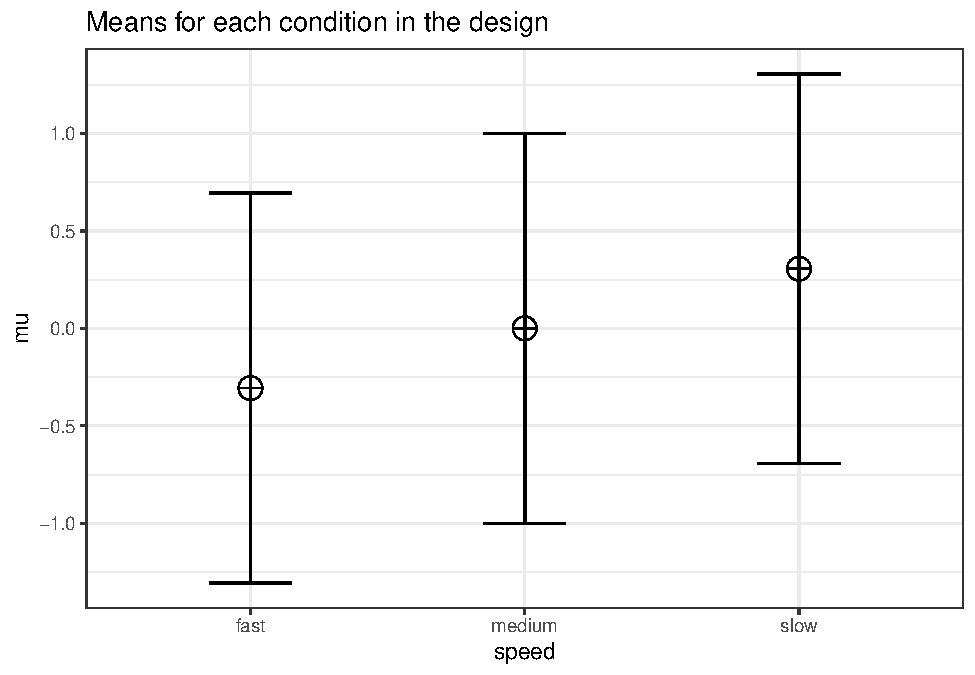
\includegraphics{SuperpowerValidation_files/figure-latex/unnamed-chunk-39-1.pdf}

\begin{Shaded}
\begin{Highlighting}[]
\NormalTok{alpha_level <-}\StringTok{ }\FloatTok{0.05}
\KeywordTok{ANOVA_power}\NormalTok{(design_result, }\DataTypeTok{nsims =}\NormalTok{ nsims)}
\end{Highlighting}
\end{Shaded}

\begin{verbatim}
## Power and Effect sizes for ANOVA tests
##             power effect_size
## anova_speed    98       0.351
## 
## Power and Effect sizes for contrasts
##                           power effect_size
## p_speed_fast_speed_medium    52      0.5183
## p_speed_fast_speed_slow     100      1.0454
## p_speed_medium_speed_slow    58      0.5029
## 
## Within-Subject Factors Included: Check MANOVA Results
\end{verbatim}

The results of the simulation are indeed very close to 96.9\%. We can see this is in line with the power estimate from Gpower:

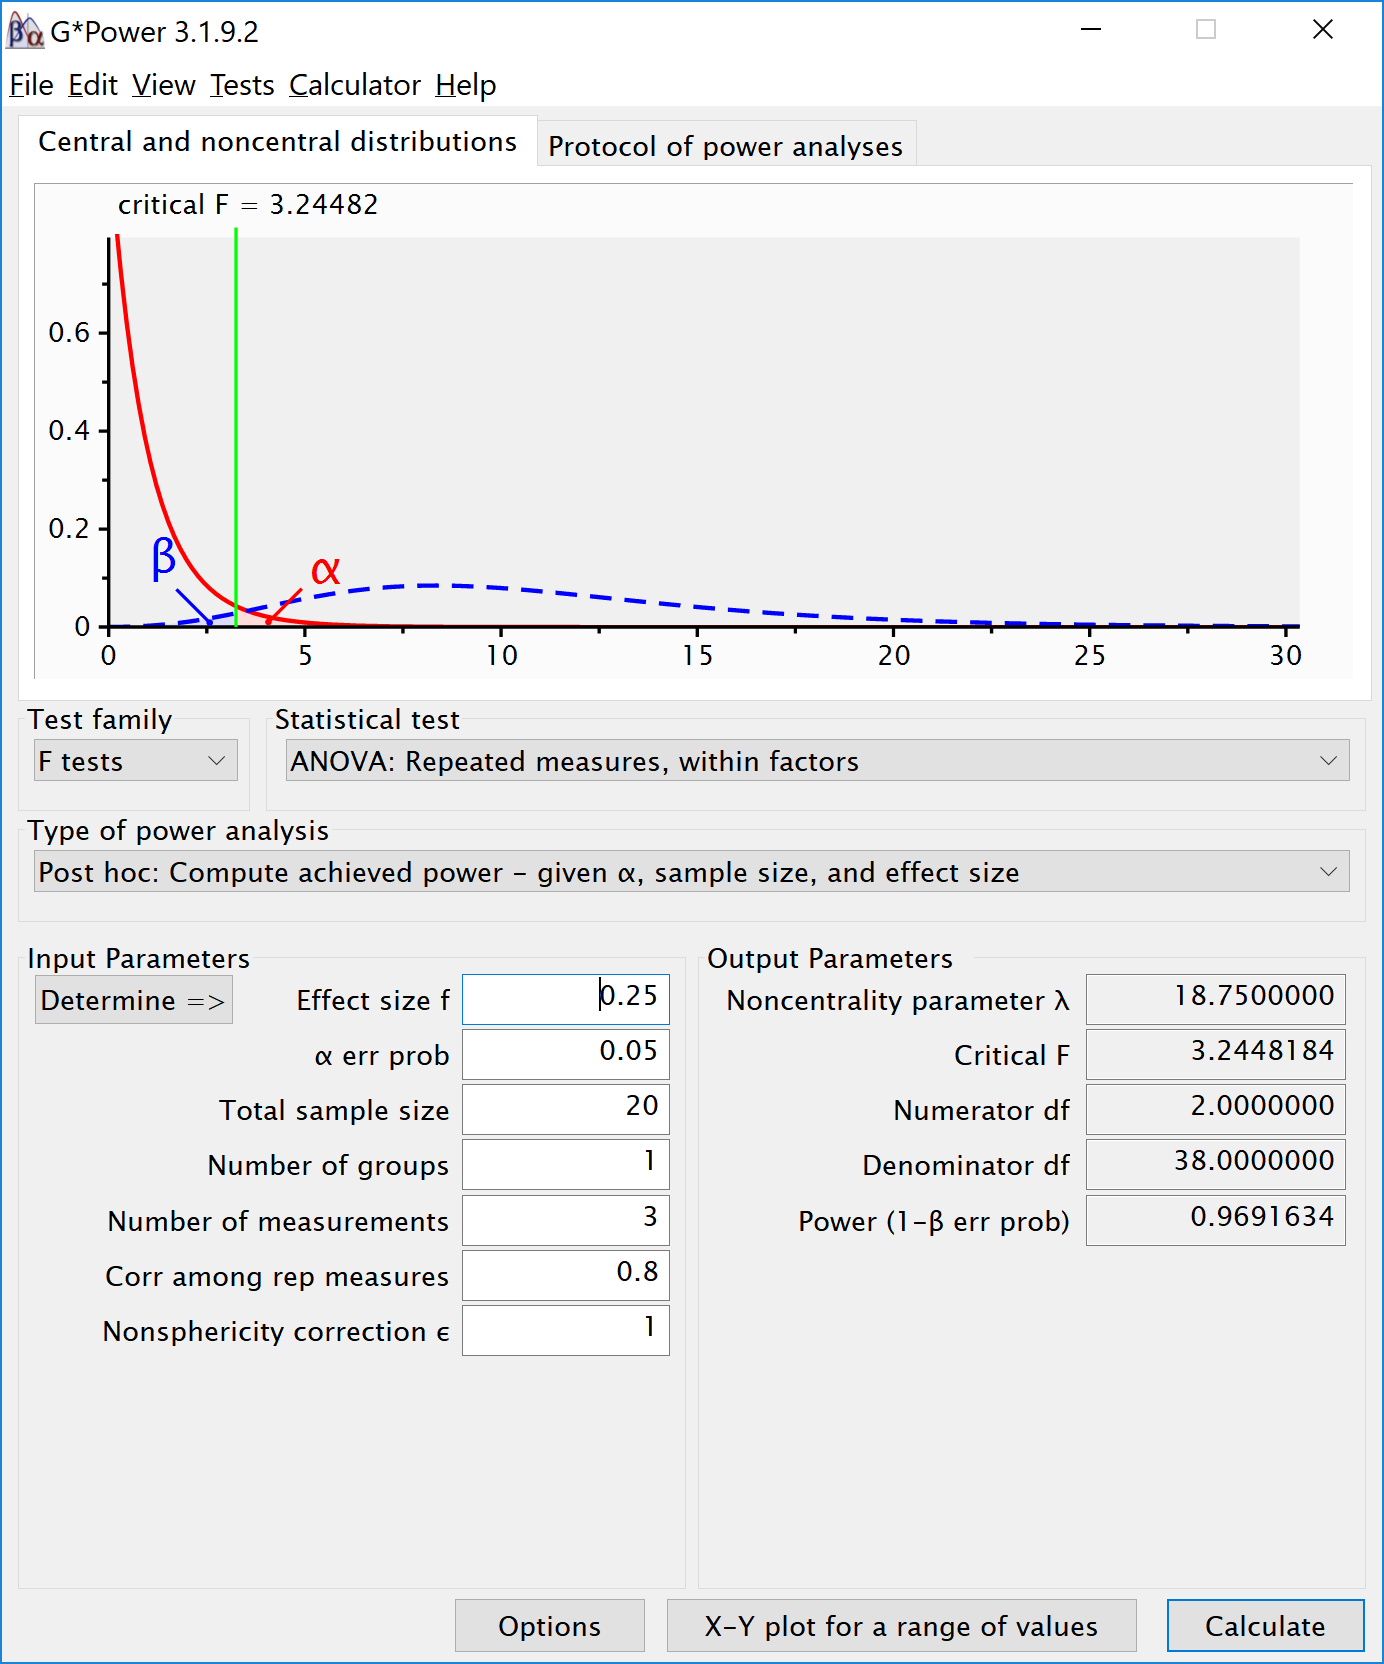
\includegraphics{screenshots/gpower_12.png}

We can also validate this by creating the code to do a power analysis in R from scratch:

\begin{Shaded}
\begin{Highlighting}[]
\NormalTok{K <-}\StringTok{ }\DecValTok{3} \CommentTok{#three groups}
\NormalTok{n <-}\StringTok{ }\DecValTok{20}
\NormalTok{sd <-}\StringTok{ }\DecValTok{1}
\NormalTok{r <-}\StringTok{ }\FloatTok{0.8}
\NormalTok{alpha =}\StringTok{ }\FloatTok{0.05}
\NormalTok{f <-}\StringTok{ }\FloatTok{0.25}
\NormalTok{f2 <-}\StringTok{ }\NormalTok{f}\OperatorTok{^}\DecValTok{2}
\NormalTok{ES <-}\StringTok{ }\NormalTok{f2}\OperatorTok{/}\NormalTok{(f2}\OperatorTok{+}\DecValTok{1}\NormalTok{)}
\NormalTok{ES}
\end{Highlighting}
\end{Shaded}

\begin{verbatim}
## [1] 0.05882353
\end{verbatim}

\begin{Shaded}
\begin{Highlighting}[]
\NormalTok{mu <-}\StringTok{ }\KeywordTok{mu_from_ES}\NormalTok{(}\DataTypeTok{K =}\NormalTok{ K, }\DataTypeTok{ES =}\NormalTok{ ES)}
\NormalTok{design =}\KeywordTok{paste}\NormalTok{(K,}\StringTok{"w"}\NormalTok{,}\DataTypeTok{sep=}\StringTok{""}\NormalTok{)}
\NormalTok{labelnames <-}\StringTok{ }\KeywordTok{c}\NormalTok{(}\StringTok{"speed"}\NormalTok{, }\StringTok{"fast"}\NormalTok{, }\StringTok{"medium"}\NormalTok{, }\StringTok{"slow"}\NormalTok{)}
\NormalTok{design_result <-}\StringTok{ }\KeywordTok{ANOVA_design}\NormalTok{(}\DataTypeTok{design =}\NormalTok{ design,}
                   \DataTypeTok{n =}\NormalTok{ n, }
                   \DataTypeTok{mu =}\NormalTok{ mu, }
                   \DataTypeTok{sd =}\NormalTok{ sd, }
                   \DataTypeTok{r =}\NormalTok{ r, }
                   \DataTypeTok{labelnames =}\NormalTok{ labelnames)}
\end{Highlighting}
\end{Shaded}

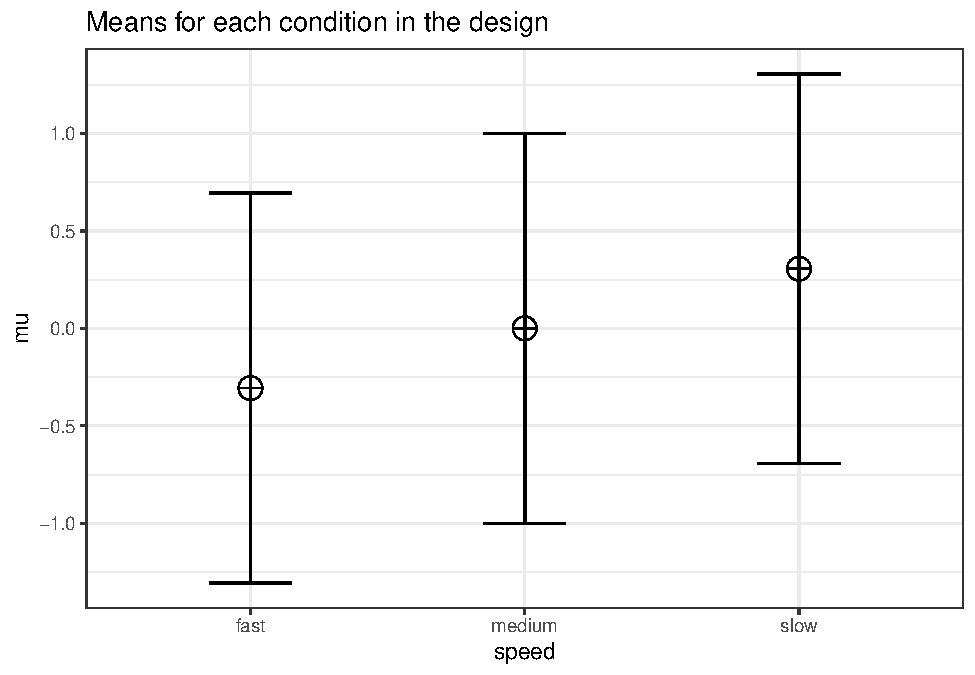
\includegraphics{SuperpowerValidation_files/figure-latex/unnamed-chunk-40-1.pdf}

\begin{Shaded}
\begin{Highlighting}[]
\KeywordTok{power_oneway_within}\NormalTok{(design_result)}\OperatorTok{$}\NormalTok{power}
\end{Highlighting}
\end{Shaded}

\begin{verbatim}
## [1] 0.9691634
\end{verbatim}

\begin{Shaded}
\begin{Highlighting}[]
\KeywordTok{power_oneway_within}\NormalTok{(design_result)}\OperatorTok{$}\NormalTok{eta_p_}\DecValTok{2}
\end{Highlighting}
\end{Shaded}

\begin{verbatim}
## [1] 0.05882353
\end{verbatim}

\begin{Shaded}
\begin{Highlighting}[]
\KeywordTok{power_oneway_within}\NormalTok{(design_result)}\OperatorTok{$}\NormalTok{eta_p_}\DecValTok{2}\NormalTok{_SPSS}
\end{Highlighting}
\end{Shaded}

\begin{verbatim}
## [1] 0.3303965
\end{verbatim}

\begin{Shaded}
\begin{Highlighting}[]
\KeywordTok{power_oneway_within}\NormalTok{(design_result)}\OperatorTok{$}\NormalTok{Cohen_f}
\end{Highlighting}
\end{Shaded}

\begin{verbatim}
## [1] 0.25
\end{verbatim}

\begin{Shaded}
\begin{Highlighting}[]
\KeywordTok{power_oneway_within}\NormalTok{(design_result)}\OperatorTok{$}\NormalTok{Cohen_f_SPSS}
\end{Highlighting}
\end{Shaded}

\begin{verbatim}
## [1] 0.7024394
\end{verbatim}

We can even check the calculation of Cohen's f SPSS style in GPower. We take the GPower settings as illustrated above. We click the `Options' button, and check the radiobutton next to `As in SPSS'. Click ok, and you will notice that the `Corr among rep measures' field has disappeared. The correlation does not need to be entered seperately, but is incorporated in Cohen's f.~The value of Cohen's f, which was 0.25, has changed into 0.7024394. This is the SPSS equivalent. The value is much larger. This value, and it's corresponding partial eta-squared, incorporate the correlation between observations.

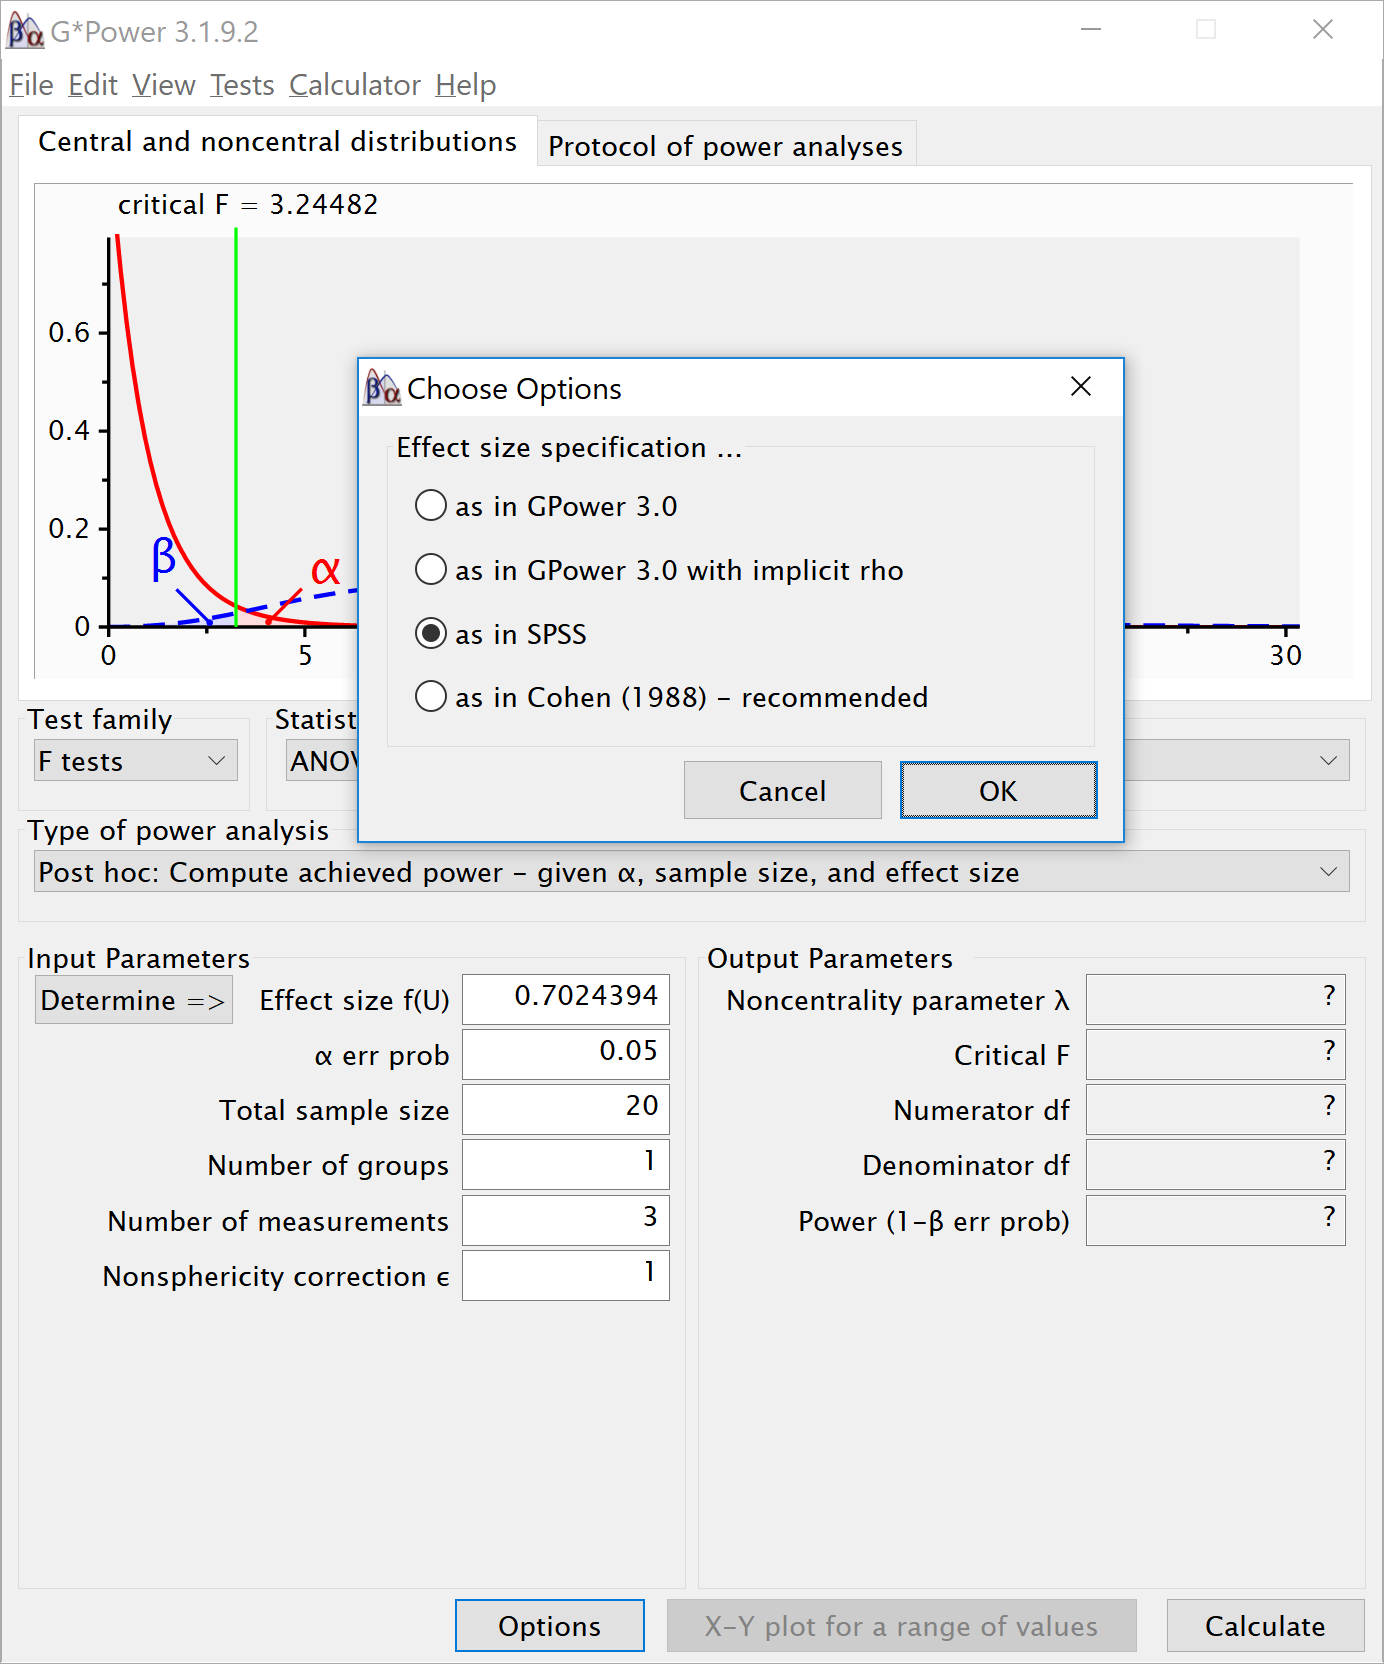
\includegraphics{screenshots/gpower_14.png}

\hypertarget{repeated-measures-anova-part-3}{%
\chapter{Repeated Measures-ANOVA Part 3}\label{repeated-measures-anova-part-3}}

We first repeat the simulation by Brysbaert:

\begin{Shaded}
\begin{Highlighting}[]
\CommentTok{# give sample size}
\NormalTok{N =}\StringTok{ }\DecValTok{75}
\CommentTok{# give effect size d}
\NormalTok{d1 =}\StringTok{ }\FloatTok{.4} \CommentTok{#difference between the extremes}
\NormalTok{d2 =}\StringTok{ }\FloatTok{.4} \CommentTok{#third condition goes with the highest extreme}
\CommentTok{# give the correlation between the conditions}
\NormalTok{r =}\StringTok{ }\FloatTok{.5}
\CommentTok{# give number of simulations}
\NormalTok{nSim =}\StringTok{ }\NormalTok{nsims}
\CommentTok{# give alpha levels}
\NormalTok{alpha1 =}\StringTok{ }\FloatTok{.05} \CommentTok{#alpha level for the omnibus ANOVA}
\NormalTok{alpha2 =}\StringTok{ }\FloatTok{.05} \CommentTok{#also adjusted from original by DL}
\CommentTok{# create progress bar in case it takes a while}
\CommentTok{#pb <- winProgressBar(title = "progress bar", min = 0, max = nSim, width = 300)}
\CommentTok{# create vectors to store p-values}
\NormalTok{p1 <-}\KeywordTok{numeric}\NormalTok{(nSim) }\CommentTok{#p-value omnibus ANOVA}
\NormalTok{p2 <-}\KeywordTok{numeric}\NormalTok{(nSim) }\CommentTok{#p-value first post hoc test}
\NormalTok{p3 <-}\KeywordTok{numeric}\NormalTok{(nSim) }\CommentTok{#p-value second post hoc test}
\NormalTok{p4 <-}\KeywordTok{numeric}\NormalTok{(nSim) }\CommentTok{#p-value third post hoc test}
\CommentTok{# open library MASS}
\KeywordTok{library}\NormalTok{(}\StringTok{'MASS'}\NormalTok{)}
\CommentTok{# define correlation matrix}
\NormalTok{rho <-}\StringTok{ }\KeywordTok{cbind}\NormalTok{(}\KeywordTok{c}\NormalTok{(}\DecValTok{1}\NormalTok{, r, r), }\KeywordTok{c}\NormalTok{(r, }\DecValTok{1}\NormalTok{, r), }\KeywordTok{c}\NormalTok{(r, r, }\DecValTok{1}\NormalTok{))}
\CommentTok{# define participant codes}
\NormalTok{part <-}\StringTok{ }\KeywordTok{paste}\NormalTok{(}\StringTok{"part"}\NormalTok{,}\KeywordTok{seq}\NormalTok{(}\DecValTok{1}\OperatorTok{:}\NormalTok{N))}
\ControlFlowTok{for}\NormalTok{(i }\ControlFlowTok{in} \DecValTok{1}\OperatorTok{:}\NormalTok{nSim)\{ }\CommentTok{#for each simulated experiment}
 \CommentTok{# setWinProgressBar(pb, i, title=paste(round(i/nSim*100, 1), "% done"))}
\NormalTok{  data =}\StringTok{ }\KeywordTok{mvrnorm}\NormalTok{(}\DataTypeTok{n=}\NormalTok{N, }\DataTypeTok{mu=}\KeywordTok{c}\NormalTok{(}\DecValTok{0}\NormalTok{, }\DecValTok{0}\NormalTok{, }\DecValTok{0}\NormalTok{), }\DataTypeTok{Sigma=}\NormalTok{rho)}
\NormalTok{  data[,}\DecValTok{2}\NormalTok{] =}\StringTok{ }\NormalTok{data[,}\DecValTok{2}\NormalTok{]}\OperatorTok{+}\NormalTok{d1}
\NormalTok{  data[,}\DecValTok{3}\NormalTok{] =}\StringTok{ }\NormalTok{data[,}\DecValTok{3}\NormalTok{]}\OperatorTok{+}\NormalTok{d2}
\NormalTok{  datalong =}\StringTok{ }\KeywordTok{c}\NormalTok{(data[,}\DecValTok{1}\NormalTok{],data[,}\DecValTok{2}\NormalTok{],data[,}\DecValTok{3}\NormalTok{])}
\NormalTok{  conds=}\StringTok{ }\KeywordTok{factor}\NormalTok{(}\KeywordTok{rep}\NormalTok{(letters[}\DecValTok{24}\OperatorTok{:}\DecValTok{26}\NormalTok{], }\DataTypeTok{each =}\NormalTok{ N))}
\NormalTok{  partID =}\StringTok{ }\KeywordTok{factor}\NormalTok{(}\KeywordTok{rep}\NormalTok{(part, }\DataTypeTok{times =} \DecValTok{3}\NormalTok{))}
\NormalTok{  output <-}\KeywordTok{data.frame}\NormalTok{(partID,conds,datalong)}
\NormalTok{  test <-}\StringTok{ }\KeywordTok{aov}\NormalTok{(datalong}\OperatorTok{~}\NormalTok{conds }\OperatorTok{+}\StringTok{ }\KeywordTok{Error}\NormalTok{(partID}\OperatorTok{/}\NormalTok{conds), }\DataTypeTok{data=}\NormalTok{output)}
\NormalTok{  tests <-}\StringTok{ }\NormalTok{(}\KeywordTok{summary}\NormalTok{(test))}
\NormalTok{  p1[i] <-}\StringTok{ }\NormalTok{tests}\OperatorTok{$}\StringTok{'Error: partID:conds'}\NormalTok{[[}\DecValTok{1}\NormalTok{]]}\OperatorTok{$}\StringTok{'Pr(>F)'}\NormalTok{[[}\DecValTok{1}\NormalTok{]]}
\NormalTok{  p2[i] <-}\StringTok{ }\KeywordTok{t.test}\NormalTok{(data[,}\DecValTok{1}\NormalTok{],data[,}\DecValTok{2}\NormalTok{], }\DataTypeTok{paired=}\OtherTok{TRUE}\NormalTok{)}\OperatorTok{$}\NormalTok{p.value}
\NormalTok{  p3[i] <-}\StringTok{ }\KeywordTok{t.test}\NormalTok{(data[,}\DecValTok{1}\NormalTok{],data[,}\DecValTok{3}\NormalTok{], }\DataTypeTok{paired=}\OtherTok{TRUE}\NormalTok{)}\OperatorTok{$}\NormalTok{p.value}
\NormalTok{  p4[i] <-}\StringTok{ }\KeywordTok{t.test}\NormalTok{(data[,}\DecValTok{2}\NormalTok{],data[,}\DecValTok{3}\NormalTok{], }\DataTypeTok{paired=}\OtherTok{TRUE}\NormalTok{)}\OperatorTok{$}\NormalTok{p.value}
\NormalTok{  \}}
\CommentTok{#close(pb)#close progress bar}
\CommentTok{#printing all unique tests (adjusted code by DL)}
\KeywordTok{sum}\NormalTok{(p1}\OperatorTok{<}\NormalTok{alpha1)}\OperatorTok{/}\NormalTok{nSim}
\end{Highlighting}
\end{Shaded}

\begin{verbatim}
## [1] 1
\end{verbatim}

\begin{Shaded}
\begin{Highlighting}[]
\KeywordTok{sum}\NormalTok{(p2}\OperatorTok{<}\NormalTok{alpha2)}\OperatorTok{/}\NormalTok{nSim}
\end{Highlighting}
\end{Shaded}

\begin{verbatim}
## [1] 0.96
\end{verbatim}

\begin{Shaded}
\begin{Highlighting}[]
\KeywordTok{sum}\NormalTok{(p3}\OperatorTok{<}\NormalTok{alpha2)}\OperatorTok{/}\NormalTok{nSim}
\end{Highlighting}
\end{Shaded}

\begin{verbatim}
## [1] 0.94
\end{verbatim}

\begin{Shaded}
\begin{Highlighting}[]
\KeywordTok{sum}\NormalTok{(p4}\OperatorTok{<}\NormalTok{alpha2)}\OperatorTok{/}\NormalTok{nSim}
\end{Highlighting}
\end{Shaded}

\begin{verbatim}
## [1] 0.06
\end{verbatim}

\hypertarget{reproducing-brysbaert}{%
\section{Reproducing Brysbaert}\label{reproducing-brysbaert}}

We can reproduce the same results as Brysbaeert finds with his code:

\begin{Shaded}
\begin{Highlighting}[]
\NormalTok{design <-}\StringTok{ "3w"}
\NormalTok{n <-}\StringTok{ }\DecValTok{75}
\NormalTok{mu <-}\StringTok{ }\KeywordTok{c}\NormalTok{(}\DecValTok{0}\NormalTok{, }\FloatTok{0.4}\NormalTok{, }\FloatTok{0.4}\NormalTok{)}
\NormalTok{sd <-}\StringTok{ }\DecValTok{1}
\NormalTok{r <-}\StringTok{ }\FloatTok{0.5}
\NormalTok{labelnames <-}\StringTok{ }\KeywordTok{c}\NormalTok{(}\StringTok{"speed"}\NormalTok{, }\StringTok{"fast"}\NormalTok{, }\StringTok{"medium"}\NormalTok{, }\StringTok{"slow"}\NormalTok{)}
\end{Highlighting}
\end{Shaded}

We create the within design, and run the simulation

\begin{Shaded}
\begin{Highlighting}[]
\NormalTok{design_result <-}\StringTok{ }\KeywordTok{ANOVA_design}\NormalTok{(}\DataTypeTok{design =}\NormalTok{ design,}
                   \DataTypeTok{n =}\NormalTok{ n, }
                   \DataTypeTok{mu =}\NormalTok{ mu, }
                   \DataTypeTok{sd =}\NormalTok{ sd, }
                   \DataTypeTok{r =}\NormalTok{ r, }
                   \DataTypeTok{labelnames =}\NormalTok{ labelnames)}
\end{Highlighting}
\end{Shaded}

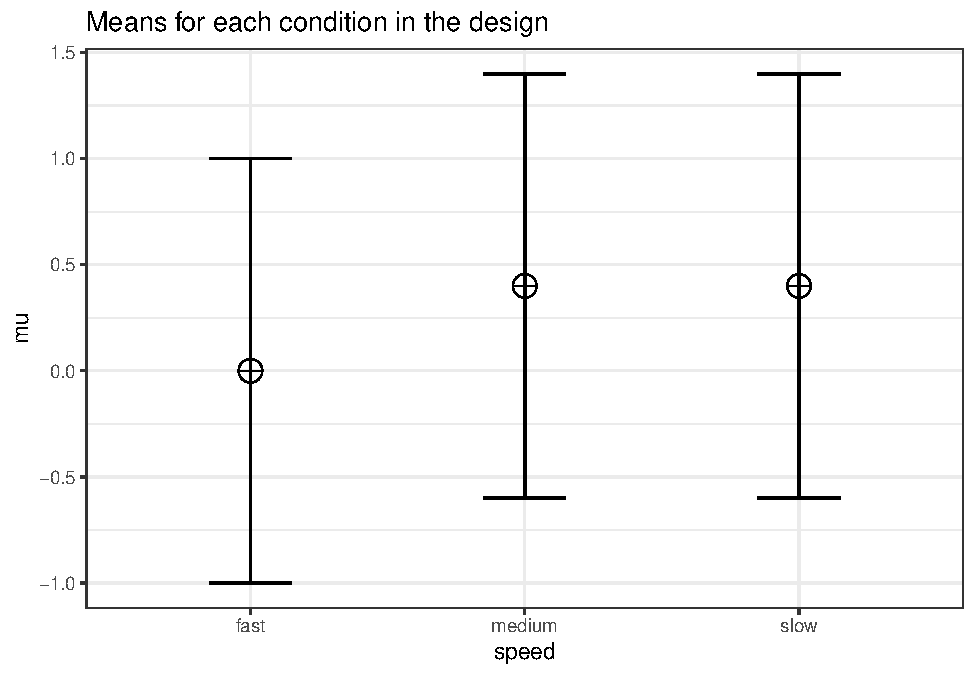
\includegraphics{SuperpowerValidation_files/figure-latex/unnamed-chunk-43-1.pdf}

\begin{Shaded}
\begin{Highlighting}[]
\KeywordTok{ANOVA_power}\NormalTok{(design_result, }\DataTypeTok{nsims =}\NormalTok{ nsims)}
\end{Highlighting}
\end{Shaded}

\begin{verbatim}
## Power and Effect sizes for ANOVA tests
##             power effect_size
## anova_speed    98      0.1108
## 
## Power and Effect sizes for contrasts
##                           power effect_size
## p_speed_fast_speed_medium    89    0.411530
## p_speed_fast_speed_slow      95    0.414675
## p_speed_medium_speed_slow     8    0.005365
## 
## Within-Subject Factors Included: Check MANOVA Results
\end{verbatim}

\#Results

The results of the simulation are very similar. Power for the ANOVA \emph{F}-test is around 95.2\%. For the three paired t-tests, power is around 92.7. This is in line with the a-priori power analysis when using g*power:

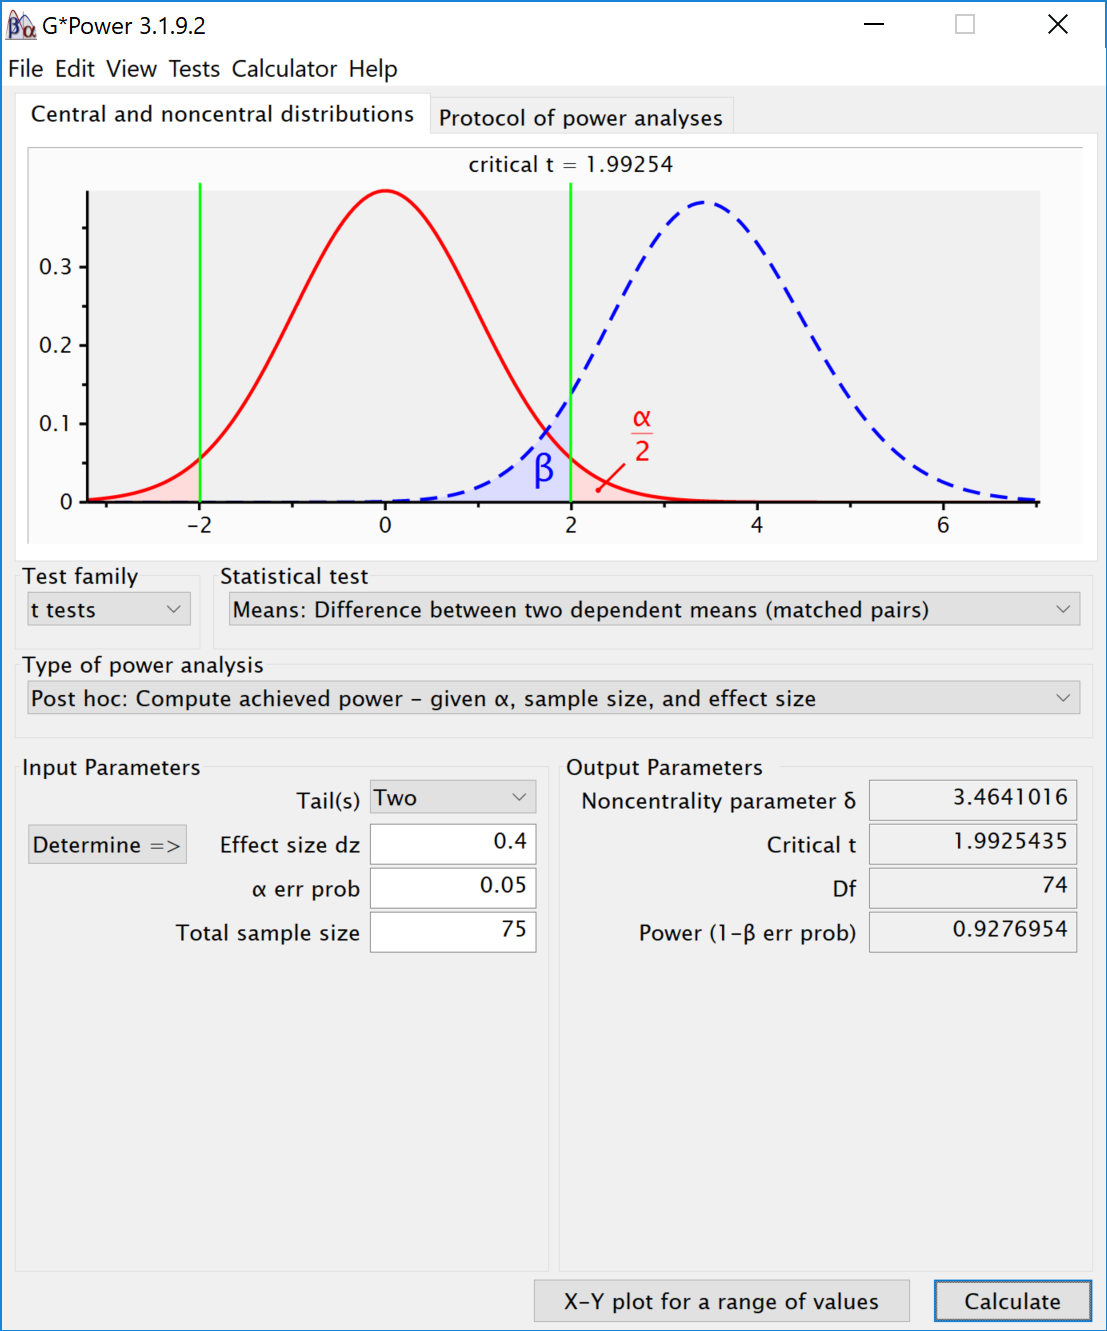
\includegraphics{screenshots/gpower_2.png}

We can perform an post-hoc power analysis in G*power. We can calculate Cohen´s f based on the means and sd, using our own custom formula.

\begin{Shaded}
\begin{Highlighting}[]
\CommentTok{# Our simulation is based onthe following means and sd:}
\CommentTok{# mu <- c(0, 0.4, 0.4)}
\CommentTok{# sd <- 1}
\NormalTok{f <-}\StringTok{ }\KeywordTok{sqrt}\NormalTok{(}\KeywordTok{sum}\NormalTok{((mu}\OperatorTok{-}\KeywordTok{mean}\NormalTok{(mu))}\OperatorTok{^}\DecValTok{2}\NormalTok{)}\OperatorTok{/}\KeywordTok{length}\NormalTok{(mu))}\OperatorTok{/}\NormalTok{sd }\CommentTok{#Cohen, 1988, formula 8.2.1 and 8.2.2}
\CommentTok{# We can see why f = 0.5*d. }
\CommentTok{# Imagine 2 group, mu = 1 and 2}
\CommentTok{# Grand mean is 1.5, we have sqrt(sum(0.5^2 + 0.5^2)/2), or sqrt(0.5/2), = 0.5. }
\CommentTok{# For Cohen's d we use the difference, 2-1 = 1. }
\end{Highlighting}
\end{Shaded}

The Cohen´s f is 0.1885618. We can enter the f (using the default 'as in G*Power 3.0' in the option window) and enter a sample size of 75, number of groups as 1, number of measurements as 3, correlation as 0.5. This yields:

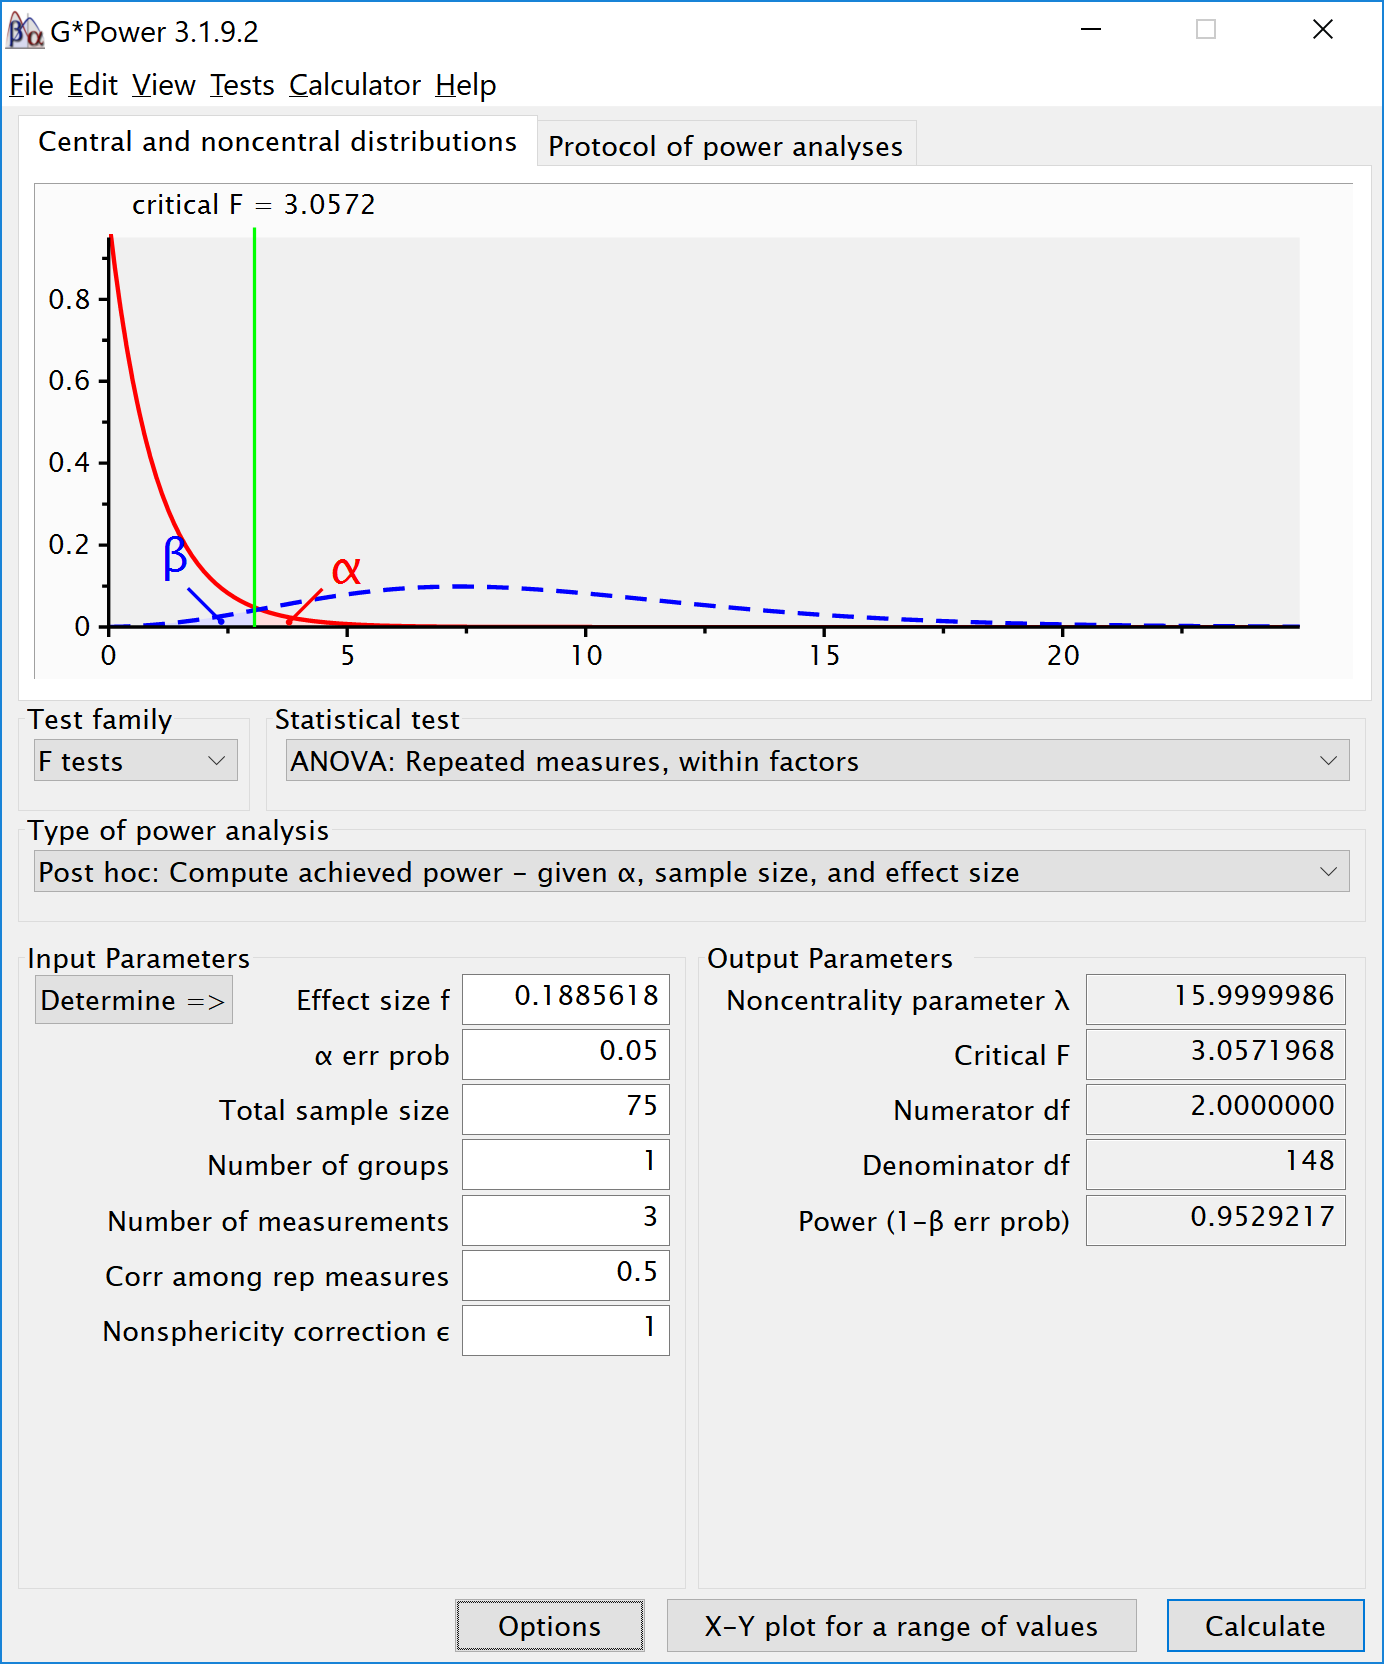
\includegraphics{screenshots/gpower_3.png}

\hypertarget{reproducing-brysbaert-variation-1-changing-correlation}{%
\section{Reproducing Brysbaert Variation 1 Changing Correlation}\label{reproducing-brysbaert-variation-1-changing-correlation}}

\begin{Shaded}
\begin{Highlighting}[]
\CommentTok{# give sample size}
\NormalTok{N =}\StringTok{ }\DecValTok{75}
\CommentTok{# give effect size d}
\NormalTok{d1 =}\StringTok{ }\FloatTok{.4} \CommentTok{#difference between the extremes}
\NormalTok{d2 =}\StringTok{ }\FloatTok{.4} \CommentTok{#third condition goes with the highest extreme}
\CommentTok{# give the correlation between the conditions}
\NormalTok{r =}\StringTok{ }\FloatTok{.6} \CommentTok{#increased correlation}
\CommentTok{# give number of simulations}
\NormalTok{nSim =}\StringTok{ }\NormalTok{nsims}
\CommentTok{# give alpha levels}
\NormalTok{alpha1 =}\StringTok{ }\FloatTok{.05} \CommentTok{#alpha level for the omnibus ANOVA}
\NormalTok{alpha2 =}\StringTok{ }\FloatTok{.05} \CommentTok{#also adjusted from original by DL}
\CommentTok{# create progress bar in case it takes a while}
\CommentTok{#pb <- winProgressBar(title = "progress bar", min = 0, max = nSim, width = 300)}
\CommentTok{# create vectors to store p-values}
\NormalTok{p1 <-}\KeywordTok{numeric}\NormalTok{(nSim) }\CommentTok{#p-value omnibus ANOVA}
\NormalTok{p2 <-}\KeywordTok{numeric}\NormalTok{(nSim) }\CommentTok{#p-value first post hoc test}
\NormalTok{p3 <-}\KeywordTok{numeric}\NormalTok{(nSim) }\CommentTok{#p-value second post hoc test}
\NormalTok{p4 <-}\KeywordTok{numeric}\NormalTok{(nSim) }\CommentTok{#p-value third post hoc test}
\CommentTok{# open library MASS}
\KeywordTok{library}\NormalTok{(}\StringTok{'MASS'}\NormalTok{)}
\CommentTok{# define correlation matrix}
\NormalTok{rho <-}\StringTok{ }\KeywordTok{cbind}\NormalTok{(}\KeywordTok{c}\NormalTok{(}\DecValTok{1}\NormalTok{, r, r), }\KeywordTok{c}\NormalTok{(r, }\DecValTok{1}\NormalTok{, r), }\KeywordTok{c}\NormalTok{(r, r, }\DecValTok{1}\NormalTok{))}
\CommentTok{# define participant codes}
\NormalTok{part <-}\StringTok{ }\KeywordTok{paste}\NormalTok{(}\StringTok{"part"}\NormalTok{,}\KeywordTok{seq}\NormalTok{(}\DecValTok{1}\OperatorTok{:}\NormalTok{N))}
\ControlFlowTok{for}\NormalTok{(i }\ControlFlowTok{in} \DecValTok{1}\OperatorTok{:}\NormalTok{nSim)\{ }\CommentTok{#for each simulated experiment}
 \CommentTok{# setWinProgressBar(pb, i, title=paste(round(i/nSim*100, 1), "% done"))}
\NormalTok{  data =}\StringTok{ }\KeywordTok{mvrnorm}\NormalTok{(}\DataTypeTok{n=}\NormalTok{N, }\DataTypeTok{mu=}\KeywordTok{c}\NormalTok{(}\DecValTok{0}\NormalTok{, }\DecValTok{0}\NormalTok{, }\DecValTok{0}\NormalTok{), }\DataTypeTok{Sigma=}\NormalTok{rho)}
\NormalTok{  data[,}\DecValTok{2}\NormalTok{] =}\StringTok{ }\NormalTok{data[,}\DecValTok{2}\NormalTok{]}\OperatorTok{+}\NormalTok{d1}
\NormalTok{  data[,}\DecValTok{3}\NormalTok{] =}\StringTok{ }\NormalTok{data[,}\DecValTok{3}\NormalTok{]}\OperatorTok{+}\NormalTok{d2}
\NormalTok{  datalong =}\StringTok{ }\KeywordTok{c}\NormalTok{(data[,}\DecValTok{1}\NormalTok{],data[,}\DecValTok{2}\NormalTok{],data[,}\DecValTok{3}\NormalTok{])}
\NormalTok{  conds=}\StringTok{ }\KeywordTok{factor}\NormalTok{(}\KeywordTok{rep}\NormalTok{(letters[}\DecValTok{24}\OperatorTok{:}\DecValTok{26}\NormalTok{], }\DataTypeTok{each =}\NormalTok{ N))}
\NormalTok{  partID =}\StringTok{ }\KeywordTok{factor}\NormalTok{(}\KeywordTok{rep}\NormalTok{(part, }\DataTypeTok{times =} \DecValTok{3}\NormalTok{))}
\NormalTok{  output <-}\KeywordTok{data.frame}\NormalTok{(partID,conds,datalong)}
\NormalTok{  test <-}\StringTok{ }\KeywordTok{aov}\NormalTok{(datalong}\OperatorTok{~}\NormalTok{conds }\OperatorTok{+}\StringTok{ }\KeywordTok{Error}\NormalTok{(partID}\OperatorTok{/}\NormalTok{conds), }\DataTypeTok{data=}\NormalTok{output)}
\NormalTok{  tests <-}\StringTok{ }\NormalTok{(}\KeywordTok{summary}\NormalTok{(test))}
\NormalTok{  p1[i] <-}\StringTok{ }\NormalTok{tests}\OperatorTok{$}\StringTok{'Error: partID:conds'}\NormalTok{[[}\DecValTok{1}\NormalTok{]]}\OperatorTok{$}\StringTok{'Pr(>F)'}\NormalTok{[[}\DecValTok{1}\NormalTok{]]}
\NormalTok{  p2[i] <-}\StringTok{ }\KeywordTok{t.test}\NormalTok{(data[,}\DecValTok{1}\NormalTok{],data[,}\DecValTok{2}\NormalTok{], }\DataTypeTok{paired=}\OtherTok{TRUE}\NormalTok{)}\OperatorTok{$}\NormalTok{p.value}
\NormalTok{  p3[i] <-}\StringTok{ }\KeywordTok{t.test}\NormalTok{(data[,}\DecValTok{1}\NormalTok{],data[,}\DecValTok{3}\NormalTok{], }\DataTypeTok{paired=}\OtherTok{TRUE}\NormalTok{)}\OperatorTok{$}\NormalTok{p.value}
\NormalTok{  p4[i] <-}\StringTok{ }\KeywordTok{t.test}\NormalTok{(data[,}\DecValTok{2}\NormalTok{],data[,}\DecValTok{3}\NormalTok{], }\DataTypeTok{paired=}\OtherTok{TRUE}\NormalTok{)}\OperatorTok{$}\NormalTok{p.value}
\NormalTok{  \}}
\CommentTok{#close(pb)#close progress bar}
\CommentTok{#printing all unique tests (adjusted code by DL)}
\KeywordTok{sum}\NormalTok{(p1}\OperatorTok{<}\NormalTok{alpha1)}\OperatorTok{/}\NormalTok{nSim}
\end{Highlighting}
\end{Shaded}

\begin{verbatim}
## [1] 0.98
\end{verbatim}

\begin{Shaded}
\begin{Highlighting}[]
\KeywordTok{sum}\NormalTok{(p2}\OperatorTok{<}\NormalTok{alpha2)}\OperatorTok{/}\NormalTok{nSim}
\end{Highlighting}
\end{Shaded}

\begin{verbatim}
## [1] 0.97
\end{verbatim}

\begin{Shaded}
\begin{Highlighting}[]
\KeywordTok{sum}\NormalTok{(p3}\OperatorTok{<}\NormalTok{alpha2)}\OperatorTok{/}\NormalTok{nSim}
\end{Highlighting}
\end{Shaded}

\begin{verbatim}
## [1] 0.95
\end{verbatim}

\begin{Shaded}
\begin{Highlighting}[]
\KeywordTok{sum}\NormalTok{(p4}\OperatorTok{<}\NormalTok{alpha2)}\OperatorTok{/}\NormalTok{nSim}
\end{Highlighting}
\end{Shaded}

\begin{verbatim}
## [1] 0.05
\end{verbatim}

\begin{Shaded}
\begin{Highlighting}[]
\NormalTok{design <-}\StringTok{ "3w"}
\NormalTok{n <-}\StringTok{ }\DecValTok{75}
\NormalTok{mu <-}\StringTok{ }\KeywordTok{c}\NormalTok{(}\DecValTok{0}\NormalTok{, }\FloatTok{0.4}\NormalTok{, }\FloatTok{0.4}\NormalTok{)}
\NormalTok{sd <-}\StringTok{ }\DecValTok{1}
\NormalTok{r <-}\StringTok{ }\FloatTok{0.6}
\NormalTok{labelnames <-}\StringTok{ }\KeywordTok{c}\NormalTok{(}\StringTok{"speed"}\NormalTok{, }\StringTok{"fast"}\NormalTok{, }\StringTok{"medium"}\NormalTok{, }\StringTok{"slow"}\NormalTok{)}
\end{Highlighting}
\end{Shaded}

We create the within design, and run the simulation

\begin{Shaded}
\begin{Highlighting}[]
\NormalTok{design_result <-}\StringTok{ }\KeywordTok{ANOVA_design}\NormalTok{(}\DataTypeTok{design =}\NormalTok{ design,}
                   \DataTypeTok{n =}\NormalTok{ n, }
                   \DataTypeTok{mu =}\NormalTok{ mu, }
                   \DataTypeTok{sd =}\NormalTok{ sd, }
                   \DataTypeTok{r =}\NormalTok{ r, }
                   \DataTypeTok{labelnames =}\NormalTok{ labelnames)}
\end{Highlighting}
\end{Shaded}

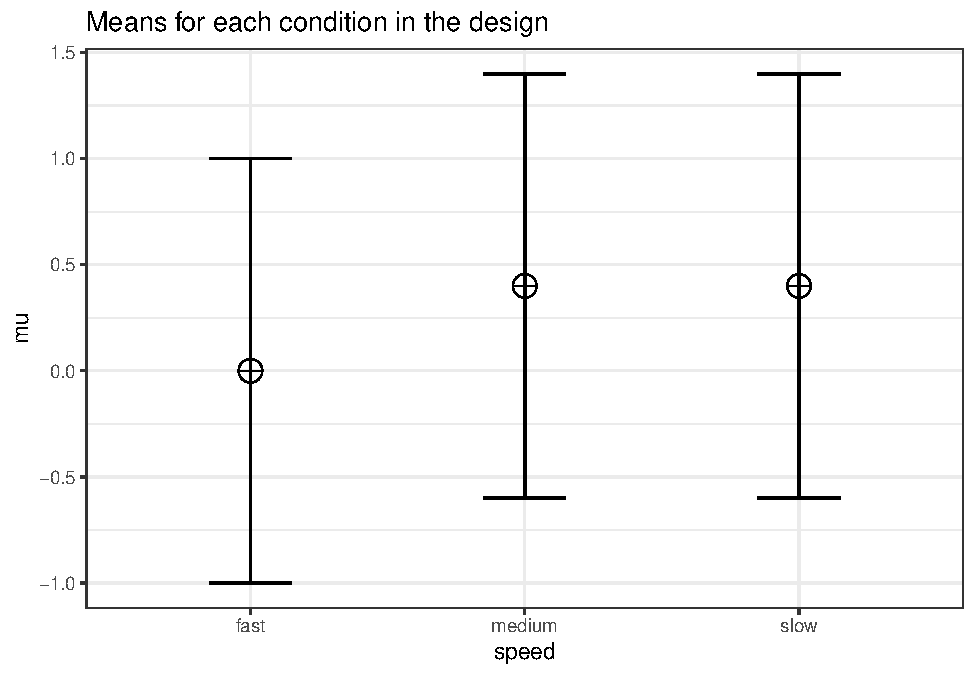
\includegraphics{SuperpowerValidation_files/figure-latex/unnamed-chunk-47-1.pdf}

\begin{Shaded}
\begin{Highlighting}[]
\KeywordTok{ANOVA_power}\NormalTok{(design_result, }\DataTypeTok{nsims =}\NormalTok{ nsims)}
\end{Highlighting}
\end{Shaded}

\begin{verbatim}
## Power and Effect sizes for ANOVA tests
##             power effect_size
## anova_speed    99      0.1307
## 
## Power and Effect sizes for contrasts
##                           power effect_size
## p_speed_fast_speed_medium    99     0.46715
## p_speed_fast_speed_slow      95     0.44372
## p_speed_medium_speed_slow     3    -0.01717
## 
## Within-Subject Factors Included: Check MANOVA Results
\end{verbatim}

Again, this is similar to g*power for the ANOVA:

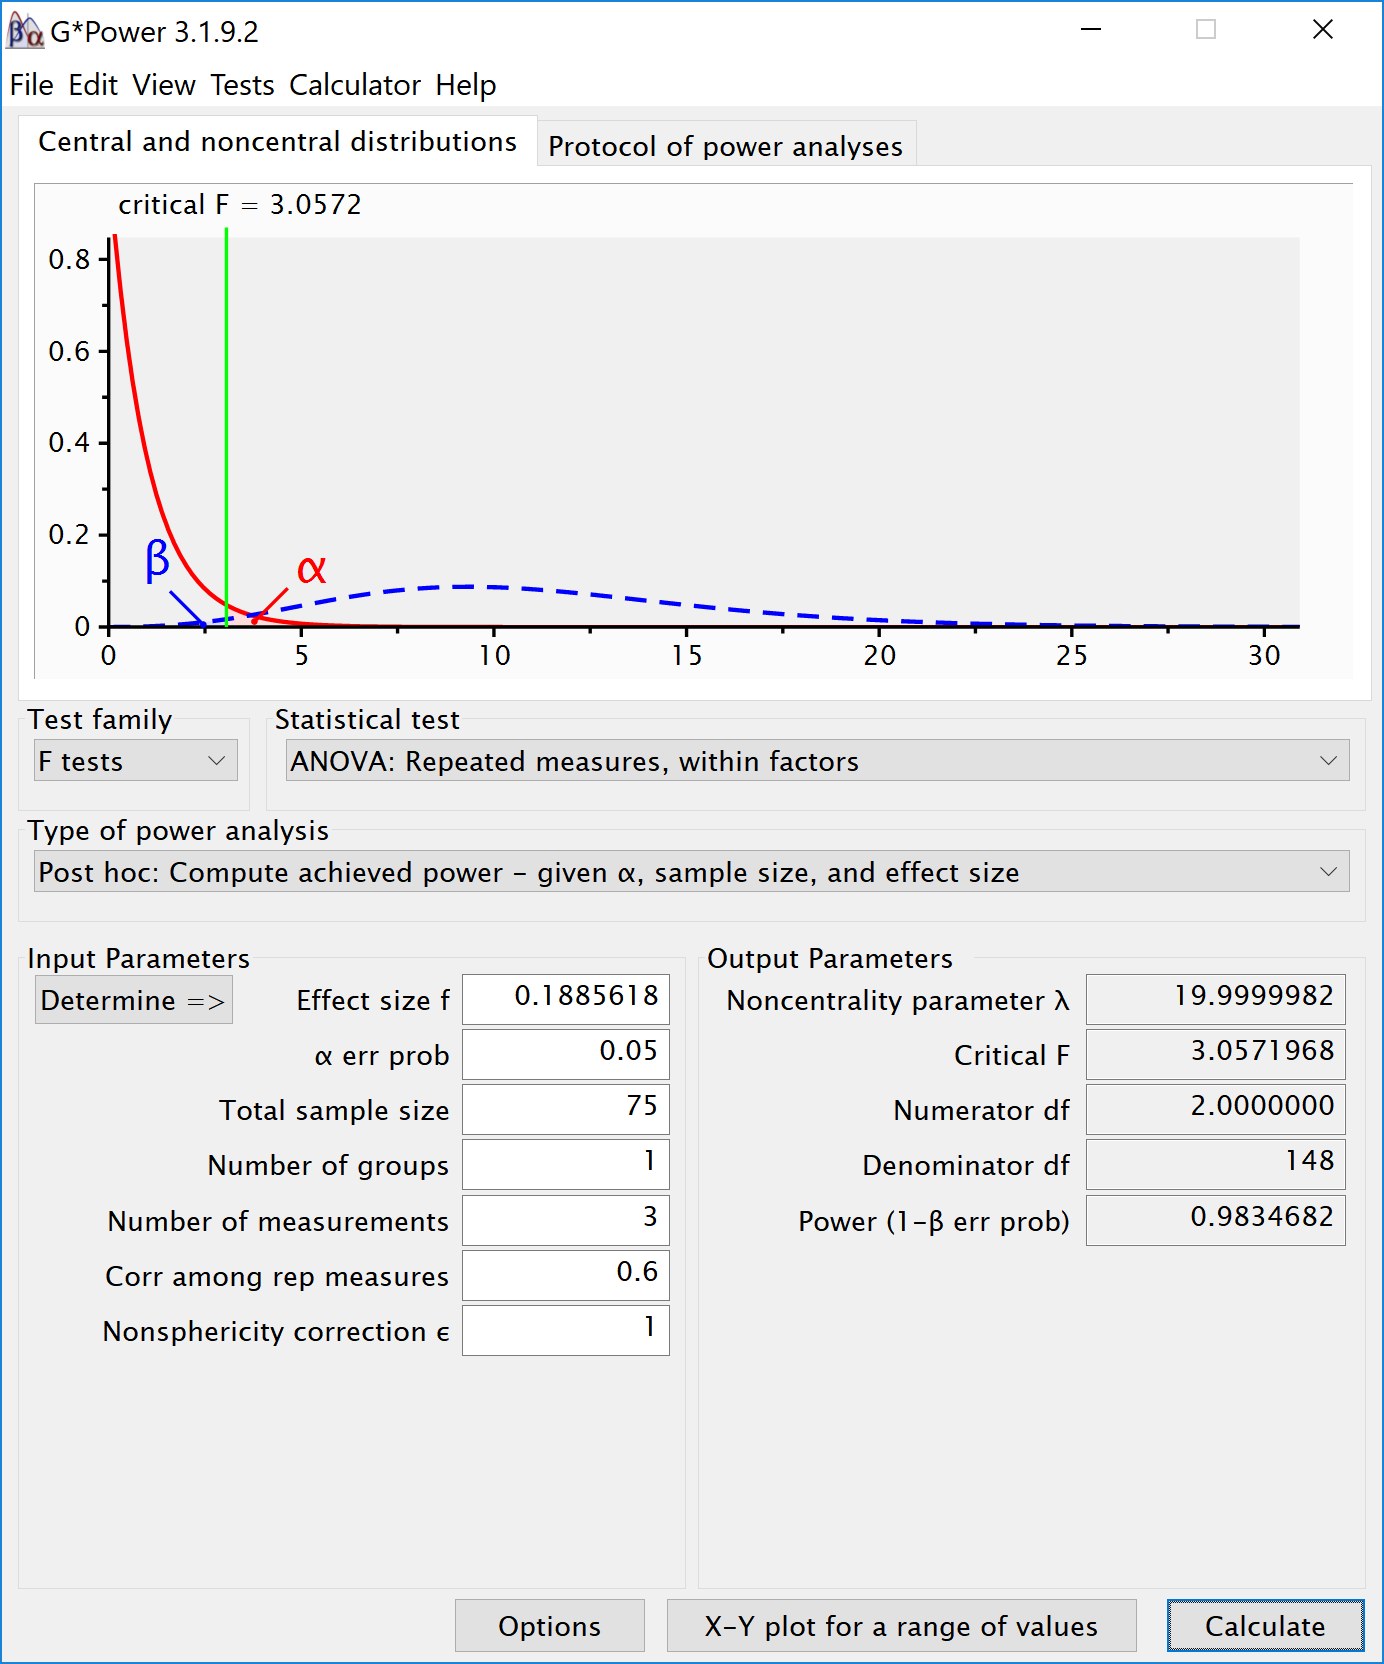
\includegraphics{screenshots/gpower_4.png}

\bibliography{book.bib,packages.bib}


\end{document}
